\documentclass[10pt]{report}
\usepackage[utf8]{inputenc}
\usepackage[italian]{babel}
\usepackage{multicol}
\usepackage{amsfonts}
\usepackage[bookmarks]{hyperref}
\usepackage[a4paper, total={18cm, 25cm}]{geometry}
\usepackage{graphicx}
\usepackage{xcolor}
\usepackage{textcomp}
\graphicspath{ {./img/} }
\usepackage{listings}
\usepackage{makecell}
\usepackage{qtree}
\usepackage{pgfplots}
\usepackage{tikz}
\usetikzlibrary{quantikz, shapes, arrows}
\usepackage{blochsphere}
\usepgflibrary{shapes}
\usepackage{cancel}
\usepgfplotslibrary{fillbetween}
\definecolor{backcolour}{RGB}{255,255,255}
\definecolor{codegreen}{RGB}{27,168,11}
\definecolor{codeblue}{RGB}{35,35,205}
\definecolor{codegray}{RGB}{128,128,128}
\definecolor{codepurple}{RGB}{205,35,56}
\lstdefinestyle{myPython}{
	backgroundcolor=\color{backcolour},   
	commentstyle=\color{codegreen},
	keywordstyle=\color{codeblue},
	numberstyle=\tiny\color{codegray},
	stringstyle=\color{codepurple},
	basicstyle=\small\ttfamily,
	breakatwhitespace=false,         
	breaklines=true,                 
	captionpos=b,                    
	keepspaces=true,                 
	numbers=left,                    
	numbersep=2pt,                  
	showspaces=false,                
	showstringspaces=false,
	showtabs=false,                  
	tabsize=2,
	language=python
}
\newcommand*\triangled[1]{\tikz[baseline=(char.base)]{
            \node[regular polygon, regular polygon sides=3,draw,inner sep=1pt] (char) {#1};}}
            
\usepackage{fancyhdr}
\pagestyle{fancy}
\renewcommand{\headrulewidth}{0pt}
\fancyhead{}
\fancyfoot[L]{Telegram: \texttt{@fexed}}
\fancyfoot[R]{Github: \texttt{fexed}}
\begin{document}
\title{Introduction to Quantum Computing}
\author{Federico Matteoni}
\date{A.A. 2021/22}
\renewcommand*\contentsname{Index}

\maketitle
\tableofcontents
\pagebreak
\section{Introduction}
Prof.: Anna Bernasconi, Gianna del Corso
\paragraph{What is Quantum Computing?} Quantum computing concerns the \textbf{relationship between physics and computer science}. Physical phenomenon apply to information and computation: a \textbf{computational process is seen as a physical process}, performed on a machine whose operation obey certain physical laws.\\
The classical theory of computation is based on the Universal Turing Machine, a mathematical abstraction and \textbf{not a physical device}, that works according to a set of rules and principles enunciated in 1936 and elaborated in the 1940s.
\subparagraph{Church-Turing Thesis} \textit{Every function which would naturally be regarded as computable can be computed by the Universal Turing Machine}.\\
A stronger version: every function that we can compute efficiently on any machine efficiently on a Universal Turing Machine. So we can solve a problem if and only if we can solve it on a Turing machine.\\\\
The assumption underlying these principles is that a Turing machine idealizes a mechanical computing device that obeys the laws of classical physics, but nature is better described by the laws of quantum physics. Feynman stated that "\textit{nature isn't classical}", and that our model of computations (i.e. classical computers) cannot efficiently model quantum systems in a scalable manner. They seem to be extraordinarily slow and inefficient at doing quantum simulations.
\paragraph{David Deutsch} "\textit{Computers are physical objects, and computations are physical processes. What computers can or cannot compute is determined by the laws of physics alone, and not pure mathematics.}"\\
Is there a single universal computing device which can efficiently simulate any other physical system? To answer this, Deutsch proposed a new type of computing system: quantum computers.\\
Quantum computers can do everything that conventional computers can do, but are also capable of efficiently simulate quantum-mechanical processes. And so they are \textbf{more natural computing models than conventional computers}.
\paragraph{What is quantum?} Quantum physics is a mathematical model first used to describe physical phenomena that occur at the microscopic level, such as inside an atom, which exposed gaps in the preceding theory of classical physics. Quantum theory explains this behavior and gives us a more complete picture of the universe. The description of the universe given by quantum physics differs in fundamental ways from the classical description, and is often at odds with our intuition which has evolved according to observation of macroscopic phenomena (which are, to an extremely good approximation, classical physics).
\subparagraph{An experiment} Let us consider an experiment that could not be explained in a natural way using classical physics. This experiment involves photons:\begin{list}{}{}
	\item elementary particles (\textbf{quantum}) of light
	\item massless
	\item move at the speed of light in vacuum ($\simeq 3\cdot10^8$ m/s)
	\item exhibit wave-particle duality: behavior featuring properties of both waves and particles
\end{list}
We need a photon source, a beam splitter (implemented using a half silvered mirror) and a pair of photon detectors. We will trace the behavior of the photons.
\begin{center}
	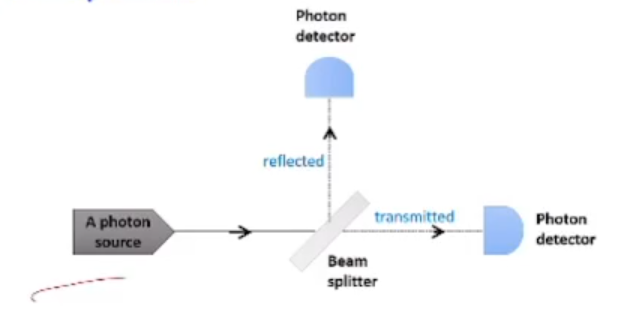
\includegraphics[scale=0.5]{1.png}
\end{center}
We send a series of individual photons along a path from the source towards the splitter. We expect two behaviors: the beam splitter transmits or reflects the photon. We observe the photon arriving at the detector on the right of the splitter half of the time, and arriving at the detector above half of the time.\\
So, we can model the splitter as flipping a fair coin, and choosing whether to transmit or reflect the photon based on the result of the coin-flip.\\\\
A beam splitter behaves like a fair coin: head (state 0) $\rightarrow$ transmitted, tail (state 1) $\rightarrow$ reflected. So both detectors will expect a photon with probability $\frac{1}{2}$
\subparagraph{Second experiment} We extend the experiment with two mirrors and another beam splitter.
\begin{center}
	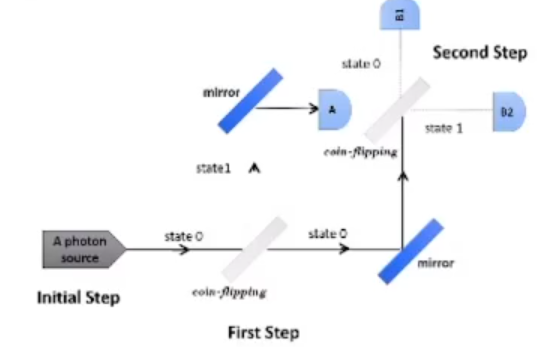
\includegraphics[scale=0.5]{2.png}
\end{center}
We have three detectors, and we observe a photon in A with probability $\frac{1}{2}$, and in B1 or B2 with probability both $\frac{1}{4}$.\\
Both experiments confirms our prediction.
\subparagraph{Third experiment} Let's remove the detector A.\begin{center}
	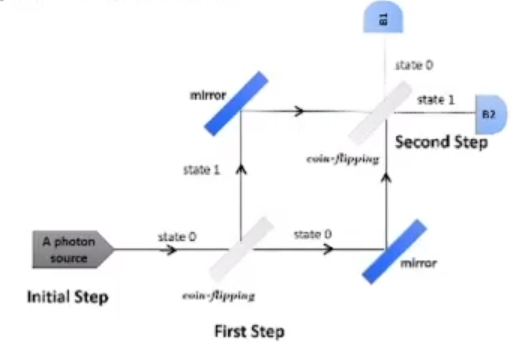
\includegraphics[scale=0.5]{3.png}
\end{center}
So we flip our photon, the "quantum coin", \textbf{without looking at the result of the first splitter}. What are the probabilities of observing the photon in B1 or B2? With the classical intuition, we expect $\frac{1}{2}$ probability in both and that's what would happen with a real "macroscopic" coin. So we predict to observe the photon in B1 and B2 evenly.\\
Let's see it in a mathematical way:
\begin{list}{}{}
	\item State 0: transmitted
	\item State 1: reflected
\end{list}
With a vector representation:
$$\ket{0} = \left(\begin{array}{c}
	1\\0
	\end{array}\right)\:\:\:\:\:\:\:\:\ket{1} = \left(\begin{array}{c}
	0\\1
	\end{array}\right)$$
With $|\:\:\rangle$ called \textbf{Dirac notation}, standard notation for states in quantum mechanics.\\
Uncertain states will be represented by linear combinations of $\ket{0}$ and $\ket{1}$
$$\alpha_0\ket{0} + \alpha_1\ket{1} = \alpha_0\left(\begin{array}{c}
1\\0
\end{array}\right) + \alpha_1\left(\begin{array}{c}
0\\1
\end{array}\right) = \left(\begin{array}{c}
\alpha_0\\\alpha_1
\end{array}\right)$$
With $\alpha_0,\alpha_1$ being the probabilities of finding the photon in state $\ket{0}$ or $\ket{1}$.\\
Since we should find the photon in exactly one path, we must have $\alpha_0+\alpha_1=1$\\\\
We model the splitter as randomly selecting whether the photon will be transmitted (state $\ket{0}$) or reflected (state $\ket{1}$)\\
After the initial step, we are in $\ket{0}$. We flip a coin (first splitter): the new probabilistic state is expected to be in both states with probability $\frac{1}{2}$
$$\frac{1}{2}\ket{0} + \frac{1}{2}\ket{1} = \left(\begin{array}{c}
\frac{1}{2}\\\frac{1}{2}
\end{array}\right)$$
The transition of a far coin can be represented by the matrix $$\left(\begin{array}{c c}
\frac{1}{2}&\frac{1}{2}\\\frac{1}{2}&\frac{1}{2}
\end{array}\right)$$
When the photon passes through the splitter, we multiply its state vector by this matrix, to derive the new state where the photon is expected to be in both states $\ket{0}$ and $\ket{1}$ with probability $\frac{1}{2}$
$$\left(\begin{array}{c c}
\frac{1}{2}&\frac{1}{2}\\\frac{1}{2}&\frac{1}{2}
\end{array}\right)\left(\begin{array}{c}
1\\0
\end{array}\right) = \left(\begin{array}{c}
\frac{1}{2}\\\frac{1}{2}
\end{array}\right) = \frac{1}{2}\left(\begin{array}{c}
1\\0
\end{array}\right) + \frac{1}{2}\left(\begin{array}{c}
0\\1
\end{array}\right)$$
Then we flip the coin again, and multiply the new state vector by the same matrix. The new probabilistic state will be the same:
$$\left(\begin{array}{c c}
\frac{1}{2}&\frac{1}{2}\\\frac{1}{2}&\frac{1}{2}
\end{array}\right)\left(\begin{array}{c}
\frac{1}{2}\\\frac{1}{2}
\end{array}\right) = \left(\begin{array}{c}
\frac{1}{2}\\\frac{1}{2}
\end{array}\right) = \frac{1}{2}\left(\begin{array}{c}
1\\0
\end{array}\right) + \frac{1}{2}\left(\begin{array}{c}
0\\1
\end{array}\right)$$
So our mathematical model confirms our expectations.\\\\
\textbf{The experimental results do not agree with our classical intuition!} We observe the photons \textbf{only in B1} and we \textbf{never observe any photon in B2}. This is the same problem which led to the development of quantum physics.
\paragraph{Quantum Physics} So let's use quantum physics to explain our experiments. "\textit{Quantum theory is probability theory with negative numbers}", but we can't have negative probabilities so we will use a new quantity called \textbf{amplitude}. To get around the fact that we cannot have negative probabilities and that all our probabilities must add up to 1, we use a mathematical trick: we square our amplitudes to calculate the probabilities.\\
According to the quantum mechanical description, the beam splitter causes the photon to go into a \textbf{superposition} of both states. Mathematically, we describe such superposition by taking a linear combination of the state vectors with $\alpha_0$ and $\alpha_1$ now being \textbf{complex numbers} $\in C$. If we measure the photon to see its state, we find it in state $\ket{0}$ with probability $|\alpha_0|^2$ and in state $\ket{1}$ with probability $|\alpha_1|^2$, and since a photon should be find in exactly one path, we need $|\alpha_0|^2+|\alpha_1|^2 = 1$\\\\
We start in state $\ket{0}=\left(\begin{array}{c}1\\0\end{array}\right)$. When it passes through the first splitter, we multiply its state vector with the matrix $$\left(\begin{array}{c c}
\frac{1}{\sqrt{2}}&\frac{1}{\sqrt{2}}\\\frac{1}{\sqrt{2}}&-\frac{1}{\sqrt{2}}
\end{array}\right)$$
After passing through the first splitter:
$$\left(\begin{array}{c c}
\frac{1}{\sqrt{2}}&\frac{1}{\sqrt{2}}\\\frac{1}{\sqrt{2}}&-\frac{1}{\sqrt{2}}
\end{array}\right)\left(\begin{array}{c}
1\\0
\end{array}\right) = \left(\begin{array}{c}
\frac{1}{\sqrt{2}}\\\frac{1}{\sqrt{2}}
\end{array}\right) = \frac{1}{\sqrt{2}}\left(\begin{array}{c}
1\\1
\end{array}\right)$$
Same as before, with $\frac{1}{\sqrt{2}}$ instead of $\frac{1}{2}$. The result correspond with the observed behavior: we measure the photon in state $\ket{0}$ with probability $\left(\frac{1}{\sqrt{2}}\right)^2=\frac{1}{2}$ and in state $\ket{1}$ with probability $\left(\frac{1}{\sqrt{2}}\right)^2=\frac{1}{2}$. The photon is in a \textbf{superposition} of states $\ket{0}$ and state $\ket{1}$, being in both states with amplitudes $\frac{1}{\sqrt{2}}$ and $\frac{1}{\sqrt{2}}$ respectively.\\
If we do not measure the state of the photon after passing through the first beam splitter, then its state remains $\frac{1}{\sqrt{2}}\left(\begin{array}{c}
1\\1
\end{array}\right)$. If the photon is allowed to pass through the second splitter before any measurement, the new state vector becomes
$$\left(\begin{array}{c c}
\frac{1}{\sqrt{2}}&\frac{1}{\sqrt{2}}\\\frac{1}{\sqrt{2}}&-\frac{1}{\sqrt{2}}
\end{array}\right)\cdot\frac{1}{\sqrt{2}}\left(\begin{array}{c}
1\\1
\end{array}\right) = \left(\begin{array}{c}
\frac{1}{2} + \frac{1}{2}\\\frac{1}{2}-\frac{1}{2}
\end{array}\right) = \left(\begin{array}{c}
1\\0
\end{array}\right)$$
The amplitude of the state $\ket{0}$ becomes 1, but the amplitude of the state $\ket{1}$ becomes 0 because \textbf{the amplitudes of finding the photon in state $\ket{1}$ cancel each other out}. We call this effect \textbf{interference}.\\
After being in both states at the same time with certain amplitudes, by passing through a second splitter the outcomes are interfered with each other: the interference can be destructive ($\frac{1}{2} - \frac{1}{2}$) or constructive ($\frac{1}{2} + \frac{1}{2}$).
\paragraph{What is Quantum Computing?} If we measure the photon, we find it coming out of state $\ket{0}$ with probability 1. Thus, after the second splitter the photon is entirely in state $\ket{0}$, which is what we observed.\\
In quantum "language": the second splitter has caused the two states (in superposition) to interfere, resulting in the cancellation of state $\ket{1}$.\\
The interference effects can be used to our advantage. We can combine operations such as the quantum coin toss to build more efficient algorithms. These algorithms can use interference effects to make the wrong answers cancel out quickly and give us high probabilities of measuring the right answer. This is the idea behind quantum computing.
\paragraph{Observations}\begin{list}{}{}
	\item This model works when the initial state is $\ket{1}$
	\item This model works also with complex numbers\\
	For instance we could use:
	\begin{list}{}{}
		\item Transition matrix: $\frac{1}{\sqrt{2}}\left(\begin{array}{c c}
		1&i\\i&1
		\end{array}\right)$
		\item Superposition of state $\ket{0}$ and $\ket{1}$: $\frac{1}{\sqrt{2}}\left(\begin{array}{c}
		i\\1
		\end{array}\right)$
		\item The model is consistent with the first and second experiment
		\begin{center}
			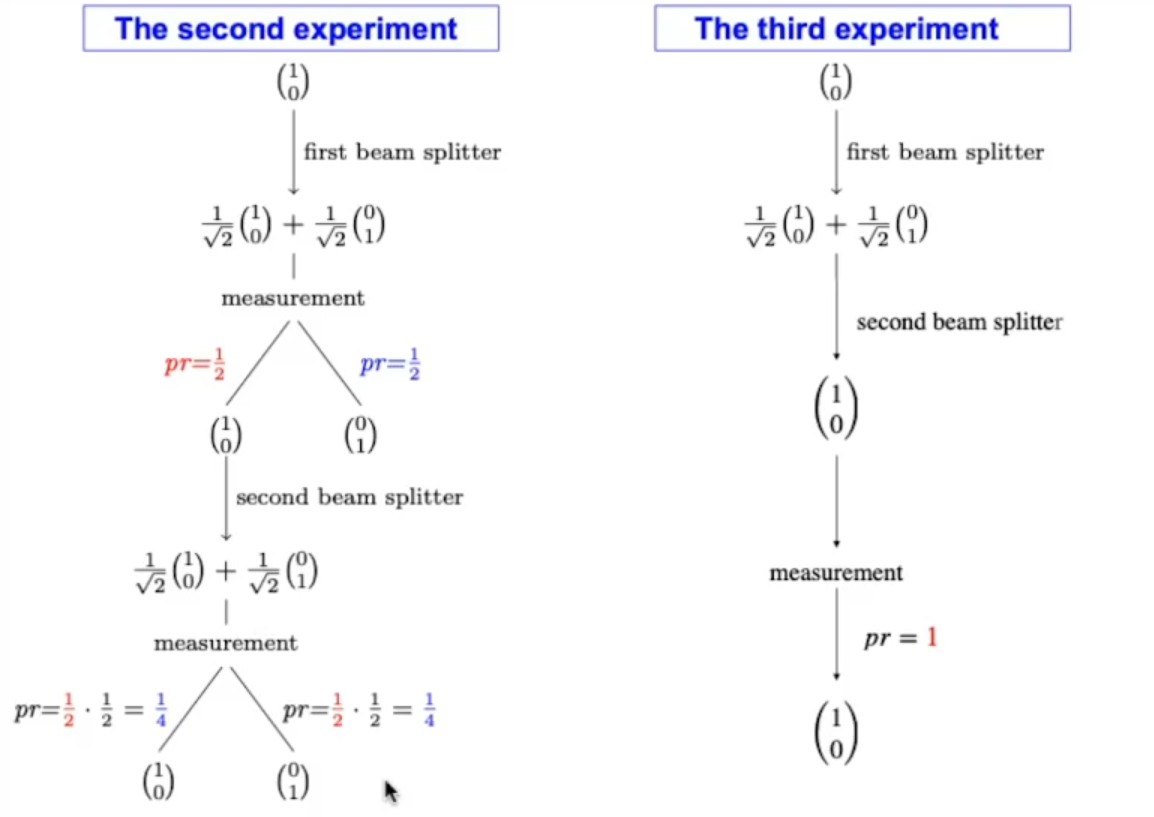
\includegraphics[scale=0.5]{4.png}
		\end{center}
	\end{list}
\end{list}
\paragraph{Phenomena of quantum mechanics that may intervene in the processing of information}
\begin{list}{}{}
	\item \textbf{Superposition} Property of a quantum system to be in different states at the same time.\\
	A quantum system can be in more than one state at the same time with non-zero amplitudes: we say that it's in a superposition of these states. When evolving from a superposition, the resulting transitions may affect each other constructively and destructively. This happens because of having opposite sign transition amplitudes
	\item \textbf{Decoherence} The attempt to observe or measure the state of the system causes its collapse towards a single state.\\
	The probability of a system to be observed in a specific state is the square value of its amplitude of a state. After the measurement, the system is no longer in a superposition: the information kept in the superposition is lost.\\
	The experimental manipulation of quantum systems is extremely difficult because every minimal disturbance can determine the decoherence.\\
	Qubits interact with their environments to some degree, even thought the physical substrate used to store them has been designed to keep the isolated.
	\item \textbf{No-Cloning} It's impossible to create an independent and identical copy of an arbitrary unknown quantum state
	\item \textbf{Entanglement} Possibility that two or more elements are in quantum states completely correlated with each other so that, even if transported at a great distance from each other, they maintain the correlation.
\end{list}
\subsection{Quantum Computer}
\paragraph{Bit and qubit} Conventional computers are made up of bits, while quantum computers are made up of quantum bits, or \textbf{qubits}.\\
A bit is the fundamental concept of classical computation: we can think of it in abstract terms as having a state which is either 0 or 1.\\
A qubit is the simplest of all quantum systems:
\begin{list}{}{}
	\item like a bit, it has a state
	\item two special states for qubits are the state $\ket{0}$ and $\ket{1}$, which correspond to states 0 and 1 of classical bits
	
$$\ket{0} = \left(\begin{array}{c}
	1\\0
	\end{array}\right)\:\:\:\:\:\:\:\:\ket{1} = \left(\begin{array}{c}
	0\\1
	\end{array}\right)$$
	These are called \textbf{computational basis states} and form an orthonormal basis for $C^2$
	\item The difference between bits and qubits is that a qubit can be in a state other than $\ket{0}$ and $\ket{1}$: it can be in a superposition of the two states simultaneously
	$$\ket{\psi} = \alpha\ket{0}+\beta\ket{1}$$
	\item The representation of information is binary, but each qubits contains double information with respect to a bit.
	\item We can examine a bit to determine if it's in state 0 or 1, but we cannot examine a qubit to determine it's quantum state (the values of $\alpha$ and $\beta$). We can only acquire much more restricted information about the quantum state.
	\item Measuring a qubit can only give classical results: either 0 with probability $|\alpha|^2$ or 1 with probability $|\beta|^2$\\
	Note that by measuring we lose information.
	\item A qubit $\ket{\psi}$ can be represented in a three-dimensional space as a point on the surface of a sphere of unitary radius known as \textbf{Bloch's sphere}.
\end{list}
\begin{center}
	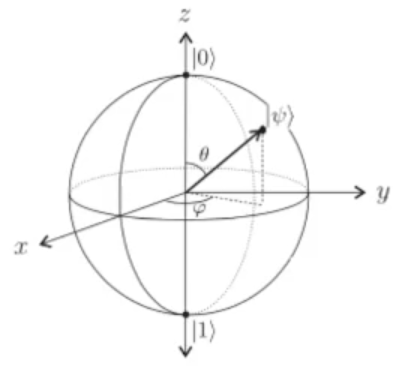
\includegraphics[scale=0.5]{5.png}
\end{center}
How much information in a qubit $\ket{\psi} = \alpha\ket{0} + \beta\ket{1}$? $\alpha$ is a complex number and we could store lots of bits in the binary expression of Re$(\alpha)$. This is there was some way of measuring the value of $\alpha$ exactly. But $\alpha,\beta$ are kind of hidden information. Measurement of a qubit will give only a single bit of information, 0 or 1, about the state of the qubit. There is no way to figure out $\alpha$ and $\beta$ if they start out unknown: after the measurement $\alpha$ and $\beta$ are gone.\\
Why does this collapse occurs? \textbf{We don't know}.\\
Only if infinitely many identically prepared qubits %TODO
\paragraph{Power of Quantum Computing} The system can be put in a combination of very large number of state: $n$ qubits in a superposition of $2^n$ states, so operating on $2^n$ bits at the same time.\\
Idea: find an algorithm that converges all $2^n$ states of the qubits to a state that's solution of the problem: exploiting constructive and destructive interferences, for example.
\paragraph{Quantum Algorithms} We start from a well known initial state (example: all qubits in $\ket{0}$). The system evolves in a quantum way: qubits are connected in elementary logic circuits and are manipulated by a simple set of rules (rotations of state vectors of the quantum state).\\
From a superposition of states to a superpositions of calculations (each with a certain probability of converging to a significant result) to a superposition of results. When the machine measures the final state, the superposition of results collapses on the result with the higher probability: with high probability being the solution of our problem.\\
This can be called \textbf{quantum parallelism}.\begin{list}{}{}
	\item Observing the system during these manipulations comes with a severe \textbf{penalty}: if we look to soon, the \textbf{computation will fail}. We are allowed to \textbf{view only the machine final state}.
	\item Interaction with the outside occurs through classic bit sequences: qubits collapses in that instant to a single state.
\end{list}
\paragraph{Why Quantum Computing?} The idea was born to efficiently simulate quantum-mechanical processes. But this model can help to solve problems of high computational complexity.\\
However:
\begin{list}{}{}
	\item Quantum computation doesn't violate the Church-Turing thesis, undecidable functions are still undecidable
	\item Widely believed that NP-Complete problems are still difficult problems, requiring exponential time
\end{list}
We are interested because for some problems a classical computers can take exponentially more time.
\paragraph{Shor's Factoring Algorithm} Factor numbers in polynomial time. This remains one of the (or \textit{the}) most important results in quantum computing. Meaning that \textbf{current public key cryptography can be attacked}. But remember that factorization is not NP-complete.
\paragraph{Grover's Quantum Search} The algorithm concerns search in an unstructured database with $N$ entries. If we are searching for a unique marked entry, classicaly it would take a maximum of $N$ queries and $\frac{N}{2}$ queries on average.\\
With this algorithm, enables the search to be completed with $O(\sqrt{N})$ queries. It's \textbf{optimal}: no search algorithm can do less than $\sqrt{N}$ operations.\\
In practice, this quadratic speed-up can be very impactful making a big difference. With $10^{20}$ entries, and a quantum processors capable of $10^8$ calls per second, we can find the entry in $10^{10}$ calls, so $10^2$ seconds ($\simeq 2$ minutes). In classical search we would need $10^{12}$ seconds ($\simeq 32000$ years).\\
In cryptography, it enables brute force attacks so we need longer keys.
\paragraph{Evolution of Quantum Technology}
%TODO image
\begin{center}
	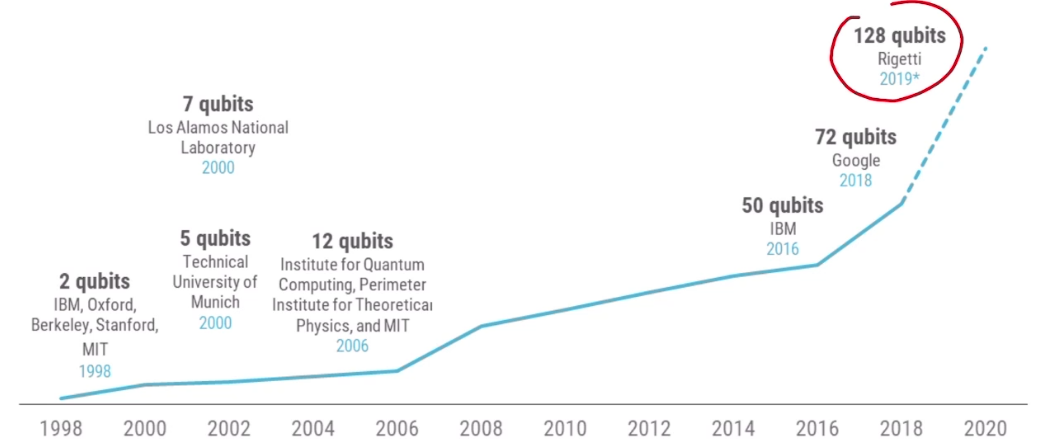
\includegraphics[scale=0.5]{6.png}
\end{center}
IBM claims that it will build a 1000-qubit machine by 2023 and 1M-qubits by 2030.
\paragraph{Quantum Supremacy} Is the goal of demonstrating that a programmable quantum device can solve a problem that \textbf{no classical computer can solve in any feasible amount of time} (irrespective of the usefulness of the problem).\\
Proving this requires:\begin{list}{}{}
	\item Building a powerful physical quantum machine
	\item Finding a problem that can be solved efficiently on a quantum computer with a superpolynomial speed-up over the best known or possible classical algorithm for that task.
\end{list}
Note that Shor's algorithm is unfeasible to be implemented with current technology, so it cannot be used to prove quantum supremacy.
\paragraph{Physical Realization of Quantum Computers}
A qubit can be realized as real quantum physical system. We can use:
\begin{list}{}{}
	\item Two different polarization of a photon
	\item Two possible alignments of nuclear spin in a uniform magnetic field
	\item Two state of an electron orbiting a single atom (ground or excited state, shining light on the electron makes it change states and even stay halfway between states)
\end{list}
The theory is independent of the physical realization of the system.
\begin{center}
	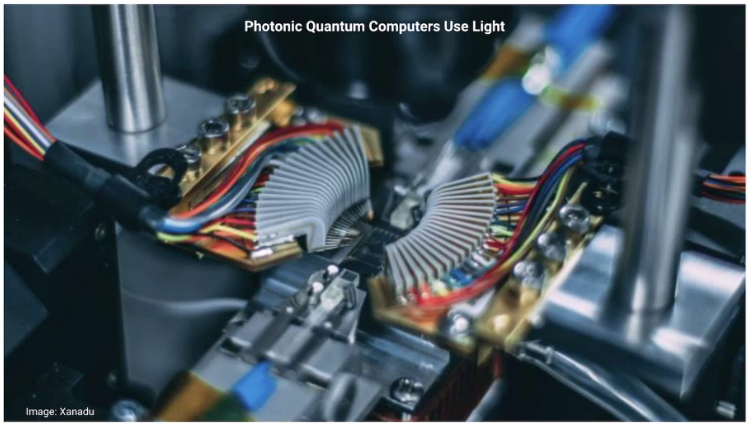
\includegraphics[scale=0.5]{7.png}
	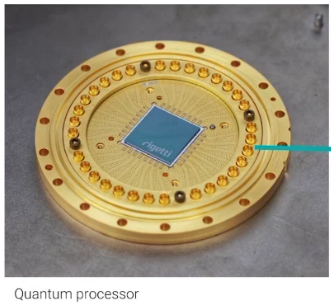
\includegraphics[scale=0.7]{8.png}
\end{center}
\paragraph{Challenges} It will be quite an engineering challenge to control a quantum computer and to make sure that its state will not be affected by various sources of error.\\
Quantum operations (rotations) are never perfect: an intended rotation of 90 degrees might end up being of 90.1 or 89.9 degrees and this errors add up quickly.\\
It's very difficult to avoid interaction with the external environments, so need fault-tollerant protocols and quantum-errors correcting algorithms, meaning additional qubits.\\
Circuit dimensions are also very large. Shor's algorithm require $O(n^2\log n\log\log n)$ gates for a $n$ bit number.
\section{Circuit Model of Computation}
\begin{center}
	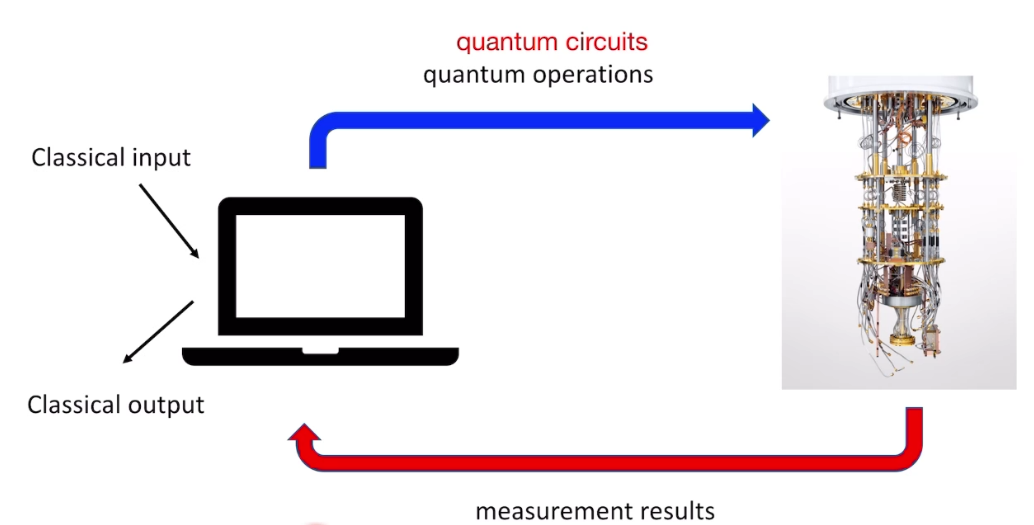
\includegraphics[scale=0.5]{9.png}
\end{center}
The \textbf{interaction is classical}.
\paragraph{Circuits} Networks (graphs) of wires (arcs) that carry bit values to gates that perform elementary operations (nodes) on the bits (input nodes).\\
$C_n$ circuit with $n$ input variables. We consider acyclic circuits. The gates come from some finite library of gates.\\
Circuits are a \textbf{non-uniform model of computation}: with $n$ inputs we can solve only instances of length $n$. Inputs of different lengths are processed by different circuits, in contrast with uniform models (such as Turing machines) where the same computational device is used for all possible input lengths. A different "program" for each input size.\\\\Non-uniform because computation on input size $n$ can be absolutely different from computations on some input size $m$. For example, \textbf{non-uniform circuit families of small size may compute undecidable functions}. Size being the number of operations in the circuit.\begin{list}{}{}
	\item Let $L\subseteq \{0,1\}^*$ be an undecidable language
	\item Let $U = \{1^n\:|\:$the binary expansion of $n$ is in $L\}$\\
	For example $1^5 = 11111_1\in U$ if $5_{10}=101_2 \in L$
	\item $U$ is also undecidable, but we can build a non-uniform family of circuits that computes $U$: $\forall\:n$ we build two circuits with $n$ inputs\begin{list}{}{}
		\item $C_n^0$ that outputs 0 if $1^n\not\in U$
		\item $C_n^1$ that outputs 1 if $1^n\in U$
	\end{list}
	What's missing is the \textbf{effective and efficient constructability} of the circuits. Since $U$ is undecidable we are not able to say if the $n$-th circuit of the family is $C_n^0$ or $C_n^1$.
\end{list}
\paragraph{Uniform Families} So we often impose a \textbf{uniformity condition}: the family is uniform if each $C_n$ can be constructed by an appropriately resource-bounded Turing machine. We assume that the circuits can be generated by a Turing machine or equivalent model that on input $n$ produces a description of $C_n$ in time polynomial in $n$ and in the number of gates in $C_n$.
\paragraph{Complexity of the Circuits} One natural measure is the \textbf{overall number of gates}, the number of operations (can be put in relation with sequential time).\\
Another is the \textbf{depth of the circuit}, the length of the longest path between input and output with each gate counting as one, can be put in relation with parallel time.\\
A third measure is the \textbf{number of input variables}, sometimes called width or space of the circuit.
\paragraph{Reversible Computation} Quantum computation are always reversible. A computation is reversible if it always possible to uniquely recover the input given the output. Otherwise, it's called irreversible.\\
Many classical logic gates are irreversible, but the NOT gate is reversible.\\
Reversibility is connected to information loss: an irreversible operation produces loss of information. With reversible computation no information is ever erased.\\
\textbf{Laws of physics are fundamentally reversible}, per out present understanding: theory of quantum computing is related to a theory of reversible computing \textbf{so quantum circuits must be reversible}.
\paragraph{Reversible Circuits} Realize bijection. We have digital circuits with same number of input and outputs. Any classical irreversible circuit can be transformed in a equivalent reversible one (computes same one), by adding new inputs and new outputs and replacing irreversible operations with reversible ones. The extra inputs represent information that we must keep in order to maintain the reversability.\\
With an irreversible classical circuit of depth $T$ and space $S$, the reversible version uses $O(S+ST)$ space and $T$ depth.
\subparagraph{Reversible AND} Also known as Toffoli gate.
\begin{center}
	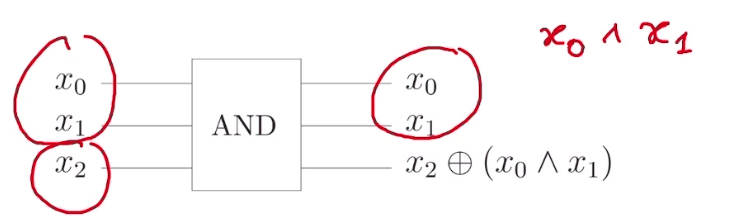
\includegraphics[scale=0.5]{10.png}
\end{center}
\paragraph{Universality} A set of gates is universal for classical computation if, for any positive integer $n,m$ and any function $f : \{0,1\}^n\rightarrow \{0,1\}^m$, a circuit can be constructed for computing $f$ using only gates from that set.\\
Well-known sets are \{AND, OR, NOT\}, \{AND, XOR, NOT\}, \{NAND\}, \{NOR\}:  NAND and NOR gates have the \textbf{functional completeness} property assuming unlimited fanout (a gate can be connected to unlimitedly many nodes).\\\\
\textbf{Toffoli gate} is universal for classical reversible computation. We need to add \textbf{ancillary} (extra) bits that can be initialized to 0 or 1 as required.
\section{Complex Numbers}
A field that can be represented in a 2D space.
$$z = a + ib$$ with $a,b \in R$ and $i^2 = -1$, that can be represented in a plot with $Re(z) = a$ on $x$ axis and $Im(z) = b$ on $y$ axis (\textbf{cartesian form}).\\
Can be expressed also as $$z = \rho(\cos\theta + i \sin\theta) = \rho \cdot e^{i\theta}$$ with $\rho$ being the distance from the origin and $\theta$ the angle (\textbf{polar form}). $\rho$ is called modulo and $e^{i\theta}$ is called phase (sometimes referring with that term to just $\theta$)
$$|z|^2 = z\cdot z^* = a^2 + b^2 = \rho^2 = |z^*|$$
$$z^* = \overline{z} = a-ib = \rho(\cos\theta - i\sin\theta) = \rho\cdot e^{-i\theta}$$
with $\overline{z}$ called complex conjugate of $z$.
\paragraph{Euler Identity} Let's prove the polar form. $e^z$ is a function from $C$ to $C$
$$e^z = \sum_{k=0}^\infty = \frac{z^k}{k!}$$
With $z\in C$, let's see with $z = ix$ and $x\in R$. We want to prove that
$$e^{ix} = \cos x + i\sin x$$
\pagebreak
$$e^{ix} = \sum_{k=0}^\infty \frac{(ix)^k}{k!} = 1 + ix + \frac{i^2x^2}{2} + \frac{i^3x^3}{3!} + \ldots=$$
Let's take the even powers, we have $i^2 = -1, i^4 = +1,\ldots$, and with the odd powers we can take out $i$ from the $\sum$
$$= \sum_{k=0}^\infty \frac{(-1)^{k}x^{2k}}{(2k)!} + i\sum_{k=0}^\infty \frac{(-1)^k x^{2k+1}}{(2k+1)!} =$$
These are the power series expansions of $\cos$ and $\sin$
$$e^{ix}=\cos x + i \sin x$$
This results in the Euler identity which puts together all the principle of math. The imaginary unit an two irrational number together with $1$ and $0$.
$$e^{i\pi} + 1 = 0 \Leftrightarrow e^{i\pi} = -1$$
\paragraph{Roots of Unity} Useful when we want to solve $z^n - 1 = 0$. We know that every polynomial has exactly $n$ roots in $C$\\
Primitive $n$th root of 1
$$\omega_n = e^{\frac{2\pi i}{n}} = \cos \frac{2\pi}{n} + i \sin\frac{2\pi}{n}$$
So for example $\omega_3 = \cos\frac{2}{3}\pi + i\sin\frac{2}{3}\pi = \frac{1}{2}+i\frac{\sqrt{3}}{2}$ for $z^3 - 1 = 0$\\
So they are counterclockwise on the unitary circle and also unitary roots are cyclic
$$w_n^k = (\cos \frac{2\pi}{n} + i \sin\frac{2\pi}{n})^k = \cos\frac{2\pi}{n}k + i \sin\frac{2\pi}{n}k = \left(e^{\frac{2\pi i}{n}}\right)^k$$
\begin{list}{}{}
	\item $\omega_n^0 = 1$
	\item $\omega_n^{n+k} = \omega_n^n \cdot \omega_n^k = \omega_n^k$
	\item $\omega_n^{n-k} = \omega_n^n \cdot \omega_n^{-k} = \omega_n^{-k}$
\end{list}
Multiplication and division are easier in the polar form
$$z_1\cdot z_2 = \rho_1\cdot\rho_2(\cos(\theta_1+\theta_2) + i\sin(\theta_1+\theta_2))$$
$$\frac{z_1}{z_2} = \frac{\rho_1}{\rho_2}(\cos(\theta_1-\theta_2) + i\sin(\theta_1-\theta_2))$$
$$z^n = \rho^n\cdot e^{in\theta}$$
\subsection{Hilbert Spaces} For Quantum Computing only finite dimensional Hilbert spaces meaning complex vector spaces with an inner product.
\paragraph{Definition} A quantum state space of a system is a vector space (complex) with inner product.\\
For example, photon polarization: we have a basis and it's a 2-dimensional space. Base states are $|\updownarrow\rangle$ and $|\leftrightarrow\rangle$. We use half-spin patches, $|\uparrow\rangle$ spin up and $|\downarrow\rangle$ spin down.\\
If we consider a 4-dimensional state space, we have $4$ vectors in the base:$\ket{0}$, $\ket{1}$, $|2\rangle$, $|3\rangle$ denoted with $$|v\rangle=\left(\begin{array}{c}
v_0\\v_1\\v_2\\v_3
\end{array}\right)$$ using the ket notation.
\paragraph{Definition} A quantum state is a vector of unitary length in a quantum state space.\\
So $\| |v\rangle\| = 1$, $\|v\|=\sqrt{(v,v)}$ with the inner product defined as
$$(v,w)=\sum_{i=1}^{d-1}v_i^*\cdot w_i$$
We can use the bra $$\langle v| = (v_0^*,\ldots,v_{d-1}^*)$$
$$\langle v\:|\:w\rangle = (v,w)\in C$$
or the ket-bra $$|v\rangle\langle w| = (v_iw_j^*)_{i,j}$$ giving a rank-one matrix.
\paragraph{} For a system of 1 qubit we have as basis $$\ket{0} = \left(\begin{array}{c}
1\\0
\end{array}\right), \ket{1}=\left(\begin{array}{c}
0\\1
\end{array}\right)$$ but we can also denote this as $|\uparrow\rangle$ and $|\downarrow\rangle$ and denote as $$|\rightarrow\rangle = \frac{|\uparrow\rangle + |\downarrow\rangle}{\sqrt{2}}$$
$$|\leftarrow\rangle = \frac{|\uparrow\rangle - |\downarrow\rangle}{\sqrt{2}}$$
as spin-right and spin-left.\\
We can define spin-in ("in the board")
$$|\otimes\rangle = \frac{|\uparrow\rangle + i|\downarrow\rangle}{\sqrt{2}}$$
and spin-out ("out of the board")
$$|\bullet\rangle = \frac{|\uparrow\rangle - i|\downarrow\rangle}{\sqrt{2}}$$
Multiplying a quantum state bu a global phase ($e^{i\theta}$) we do not change the nature of the quantum state. A global phase is a quantity that multiply all the components of the basis vector.
$$|\rightarrow\rangle = \frac{|\uparrow\rangle + |\downarrow\rangle}{\sqrt{2}} \neq \frac{|\uparrow\rangle + i|\downarrow\rangle}{\sqrt{2}} = |
\otimes\rangle$$
In the above case, $i$ is a relative phase.
\paragraph{Bloch Sphere} %TODO
\begin{center}
	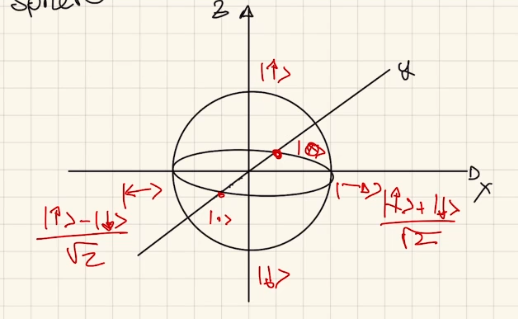
\includegraphics[scale=0.5]{11.png}
\end{center}
\paragraph{Pauli Matrices} $$X = \sigma_x = \left(\begin{array}{c c}
0&1\\1&0
\end{array}\right)$$
$$\sigma_x\ket{0} = \left(\begin{array}{c c}
0&1\\1&0
\end{array}\right)\cdot\left(\begin{array}{c}
1\\0
\end{array}\right) = \left(\begin{array}{c}
0\\1
\end{array}\right) =\ket{1}$$
It reflects the points along the $x$ axis. The same goes for $\sigma_x\ket{1} = \ket{0}$.\\
So for the points on the $x$ axis stay almost the same.
$$|\rightarrow\rangle = \frac{\ket{0} + \ket{1}}{\sqrt{2}} = \frac{1}{\sqrt{2}}\left(\begin{array}{c}
1\\1
\end{array}\right)$$
$$\sigma_x|\rightarrow\rangle = \frac{1}{\sqrt{2}}\left(\begin{array}{c}
1\\1
\end{array}\right)$$
The $y$ axis Pauli matrix is $$Y = \sigma_y = \left(\begin{array}{c c}
0&-i\\i&0
\end{array}\right) = -i\ket{0}\langle1| + i \ket{1}\langle0|$$
and the last is $$Z = \sigma_z = \left(\begin{array}{c c}
1&0\\0&-1
\end{array}\right) = \ket{0}\langle0| - \ket{1}\langle1|$$
\subparagraph{Theorem} The three Pauli matrices anticommutes
$$\sigma_i\sigma_j = -\sigma_j\sigma_i$$
for $i,j\in\{x,y,z\}$ and $i\neq j$\\
Also $\sigma_i^2 = I$
\paragraph{Hadamard Matrix} Another important matrix, used for building entangled states.
$$H=\frac{1}{\sqrt{2}}\left(\begin{array}{c c}
1&1\\1&-1
\end{array}\right)$$
It allow to move from the canonical basis to the right-left basis (also known as +- basis).
$$H\ket{0} = \frac{1}{\sqrt{2}}\left(\begin{array}{c}
1\\1
\end{array}\right) = |\rightarrow\rangle = \ket{+}$$
$$H\ket{1} = \frac{1}{\sqrt{2}}\left(\begin{array}{c}
1\\-1
\end{array}\right) = |\leftarrow\rangle = \ket{-}$$
Also $H^2 = I$, $H^{-1} = H$ so $\ket{0}\mapsto_H \ket{+}$ and $\ket{+}\mapsto_H \ket{0}$ same with $\ket{1}$ and $\ket{-}$, "back and forth".\\
$$H|\otimes\rangle = \frac{1}{\sqrt{2}}\left(\begin{array}{c c}
1&1\\1&-1
\end{array}\right)\left(\begin{array}{c}
\frac{1}{\sqrt{2}}\\\frac{1}{\sqrt{2}}i
\end{array}\right) = |\bullet\rangle$$
\paragraph{Other common single qubit gates} Already mentioned $X,Y,Z,H$\begin{list}{}{}
	\item $I = \left(\begin{array}{c c}
	1&0\\0&1
	\end{array}\right)$
	\item $S = \left(\begin{array}{c c}
	1&0\\0&e^{i\frac{\pi}{2}}
	\end{array}\right)$
	\item $T = \left(\begin{array}{c c}
	1&0\\0&e^{i\frac{\pi}{4}}
	\end{array}\right)$
\end{list}
\paragraph{Applying a Gate to a Superposition}
$$\alpha\ket{0} + \beta\ket{1} \mapsto \sigma_x\left(\begin{array}{c}
\alpha\\\beta
\end{array}\right) = \beta\ket{0} + \alpha\ket{1}$$
$$\alpha\ket{0} + \beta\ket{1} \mapsto \sigma_y\left(\begin{array}{c}
\alpha\\\beta
\end{array}\right) = -\beta i\ket{0} + \alpha i\ket{1}$$
$$\alpha\ket{0} + \beta\ket{1} \mapsto \sigma_z\left(\begin{array}{c}
\alpha\\\beta
\end{array}\right) = \alpha\ket{0} - \beta\ket{1}$$
$$\alpha\ket{0} + \beta\ket{1} \mapsto H\left(\begin{array}{c}
\alpha\\\beta
\end{array}\right) = \alpha\left(\frac{\ket{0} + \ket{1}}{\sqrt{2}}\right) + \beta\left(\frac{\ket{0} - \ket{1}}{\sqrt{2}}\right)$$
$$\alpha\ket{0} + \beta\ket{1} \mapsto S\left(\begin{array}{c}
\alpha\\\beta
\end{array}\right) = \alpha\ket{0} + \beta i\ket{1}$$
$$\alpha\ket{0} + \beta\ket{1} \mapsto T\left(\begin{array}{c}
\alpha\\\beta
\end{array}\right) = \alpha\ket{0} + e^{i\frac{\pi}{4}}\beta\ket{1}$$
To really play with qubits we introduce \textbf{unitary transformations}.
\paragraph{Unitary Transformations} A unitary transformation is a transformation mapping unit-vectors to unit-vectors. We are interested in some properties of these unitary transformation.\\
$d$-dimensional quantum state space, it's a vector space so we have a basis: we label the vectors of the base as $$\ket{0}, \ket{1},\ldots,|d-1\rangle$$
$$|j\rangle = \left(\begin{array}{c}
0\\\vdots\\0\\1\\0\\\vdots\\0
\end{array}\right)\hbox{ with }1\hbox{ in }j\hbox{th position}$$
The unitary transformation is $U = [c_0,\ldots,c_{d-1}]$ so we have $U|j\rangle = |c_j\rangle$: $c_j$ is an unit-vector, because $U$ is a unitary transformation:
\begin{list}{}{}
	\item[1.] $c_j$ is a unit-vector\\All the columns are unit vectors
	\item[2.] We can decompose $U$ as sum of rank-1 matrices
\end{list}
$$U=\sum_{k=0}^{d-1}|c_k\rangle\langle k| = |c_0\rangle\langle 0| + |c_1\rangle\langle 1| + \ldots$$
The matrix $|c_i\rangle\langle i|$ for example is of all 0s with $c_i$ in the $i$th column. $$U|j\rangle = \sum_{k=0}^{d-1}|c_k\rangle\langle k\:|\:j\rangle = \sum_{k=0}^{d-1} |c_k\rangle\delta_{kj}$$
With $\langle k\:|\:j\rangle$ inner product $\in C$ and $\delta_{kj} = \left\{\begin{array}{l l}
0&k\neq j\\
1&k = j
\end{array}\right.$\\
We can apply $U$ to combinations, for example $$U\left(\frac{|k\rangle + |j\rangle}{\sqrt{2}}\right) = \frac{1}{\sqrt{2}}(|c_k\rangle + |c_j\rangle)$$
$$\frac{1}{2}(\langle c_k|+\langle c_j|)(|c_k\rangle + |c_j\rangle) = \frac{1}{2}\left(\langle c_k\:|\:c_k\rangle + \langle c_j\:|\:c_k\rangle + \langle c_k\:|\:c_j\rangle + \langle c_j\:|\:c_j\right)=1$$
$\langle c_j\:|\:c_k\rangle + \langle c_k\:|\:c_j\rangle \in R$ meaning that $\langle c_j\:|\:c_k\rangle$ is pure immaginary, $\in C\setminus R$\\\\
We can also do with relative phases, for example $i|j\rangle$ $$U\left(\frac{|k\rangle + i|j\rangle}{\sqrt{2}}\right) = \frac{1}{\sqrt{2}}\left(|c_k\rangle + i|c_j\rangle\right) = \ldots$$
Ending up with the fact that $\langle c_j\:|\:c_k\rangle$ must be $\in R$.\\
But we have the same quantity pure immaginary and pure real, meaning that $\langle c_j\:|\:c_k\rangle = 0$
\begin{list}{}{}
	\item[3.] Columns of $U$ are orthogonal and also orthonormal
	\item[4.] Rows of $U$ are orthonormal ($\Rightarrow$ orthogonal)
	\item[5.] $U^{-1} = U^H$ \textbf{very important}
\end{list}
$$(U^H)_{ij} = u^*_{ji}$$
And $U^H = U^* =U ^+$, $U^H$ is the conjugate transpose. Diagonal conjugate, invert triangles and transpose elements. An example with an arbitrary, non unitary, matrix:
$$A=\left[\begin{array}{c c}
1+i&2-i\\3+2i&4
\end{array}\right]\Leftrightarrow A^H=\left[\begin{array}{c c}
1-i & 3-2i\\2+i&4
\end{array}\right]$$
\paragraph{Spectral Theorem} There are classes of matrices which have an orthonormal basis of eigenvectors, i.e. are diagonalizable by means of orthogonal matrices.\\
$A = A^T$ symmetric matrices. $\exists$ a orthogonal such that $A = QDQ^T$ with $D$ diagonal matrix with the eigenvalues $\lambda_i$ on the diagonal.\\
$A = A^H$ hermitan matrices, $AA^H = A^HA$\\
\textbf{Unitary matrices are normal matrices}.\\
\textbf{Spectral theorem}: a matrix $A$ is normal $\Leftrightarrow$ $\exists\:U$ unitary and $D$ diagonal $|\:A=UDU^H$, meaning that $Au_i = \lambda_iu_i\:\forall\:i=1,\ldots,n$, i.e. the columns of $U$ are an orthonormal basis of eigenvectors and $\lambda_i$ are the corresponding eigenvalues.
$$A \in C^{n\times n} = UDU^H = \sum_{k=1}^n\lambda_k|u_k\rangle\langle u_k| $$
$$U = [u_1\:|\:\ldots\:|\:u_n]$$
$|u_k\rangle\langle u_k|$ is an example of a \textbf{orthogonal projector} onto the eigenspace corresponding to $\lambda_k$
\paragraph{Evaluation of  systems}
\begin{enumerate}
	\item Isolated processes have a unitary evolution\\
	$|\psi_0\rangle\mapsto|\psi_1\rangle = U_0|\psi_0\rangle\mapsto\ldots$
	\item From time to time the process is "observed", for example with an experiment: this is called \textbf{measurement}.
\end{enumerate}
\paragraph{Rotations} Of an arbitrary angle $\Theta$ around an axis. Three different rotations, for three different axis.\\
A rotation is a unitary matrix that can always be expressed $R_x = e^{-i\frac{\Theta}{2}}x$ (example for axis $x$, same for $z$ and $y$)\\
If $A$ is normal then $A = UDU^H$, so the \textbf{exponential of a matrix} $$e^A = U\left(\sum_{k=1}^\infty \frac{D^{k}}{k!}\right) U^H = Ue^DU^H$$
For example, and since $z$ is diagonal $$R_z(\Theta) = e^{-i\frac{\Theta}{2}z} = \left(\begin{array}{c c}
e^{-i\frac{\Theta}{2}} & 0\\
0 & e^{i\frac{\Theta}{2}}
\end{array}\right) = e^{-i\frac{\Theta}{2}}\left(\begin{array}{c c}
1 & 0\\
0 & -e^{i\Theta}
\end{array}\right)$$
We get that $R_x(\Theta)=(\cos\frac{\Theta}{2})I - i\sin\frac{\Theta}{2}X$, and in general $$R_M(\Theta)=\left(\cos\frac{\Theta}{2}\right)I - i\sin\frac{\Theta}{2}M$$
To diagonalize the matrix $\sigma_i$
$$U\sigma_i U^H = D \Rightarrow e^{-i\frac{\Theta}{2}D}$$
$$U^He^{-i\frac{\Theta}{2}D}U = e^{-i\frac{\Theta}{2}\sigma_i}$$
\paragraph{Theorem} Suppose $U$ is a 1-qubit unitary gate, then there exists real numbers $\alpha,\beta,\gamma,\delta$ such that you can write $U$ like $$U=e^{i\alpha}R_z(\beta)R_y(\gamma)R_z(\delta)$$
$$\Updownarrow$$
$$U = e^{i\alpha}\left[\begin{array}{c c}
e^{-i\frac{\beta}{2}}&0\\0&e^{i\frac{\beta}{2}}
\end{array}\right]\left[\begin{array}{c c}
\cos\frac{\gamma}{2}&-\sin\frac{\gamma}{2}\\\sin\frac{\gamma}{2}&\cos\frac{\gamma}{2}
\end{array}\right]\left[\begin{array}{c c}
e^{-i\frac{\delta}{2}}&0\\0&e^{i\frac{\delta}{2}}
\end{array}\right]$$
Two rotations around $z$ and one around $y$. Any unitary can be decomposed as a product of three rotations times a phase factor.
\paragraph{Standard Rotations}
The standard rotation gates are those that define rotations around the Pauli matrices $X, Y, Z$ and are defined as $$R_P(\theta) = e^{-i\theta\frac{P}{2}} = \cos\left(\frac{\theta}{2}\right)I-i\sin\left(\frac{\theta}{2}\right)P$$
For the $x$ axis
$$R_x(\theta) = \left(\begin{array}{c c}
\cos\left(\frac{\theta}{2}\right)&-i\sin\left(\frac{\theta}{2}\right)\\
i\sin\left(\frac{\theta}{2}\right)&\cos\left(\frac{\theta}{2}\right)
\end{array}\right)$$
For the $y$ axis
$$R_y(\theta) = \left(\begin{array}{c c}
\cos\left(\frac{\theta}{2}\right)&-\sin\left(\frac{\theta}{2}\right)\\
\sin\left(\frac{\theta}{2}\right)&\cos\left(\frac{\theta}{2}\right)
\end{array}\right)$$
For the $z$ axis
$$R_z(\theta) = \left(\begin{array}{c c}
e^{-i\theta\frac{P}{2}}&0\\
0&e^{i\theta\frac{P}{2}}
\end{array}\right)$$
\paragraph{Tensor Products} Way of putting vectors together to form larger Hilbert/vector spaces.\\
Let's assume 2 qubits. The state space of these 2 qubits?
$$|00\rangle\:\:|01\rangle\:\:|10\rangle\:\:|11\rangle$$
The state space dimension is $4$. Which is the dimension of $n$ qubits? Gives us a state space $2^n$.\\
$|01\rangle_{AB} = \ket{0}_A\ket{1}_B = \ket{0}_A\otimes\ket{1}_B$ tensor product.
$$\left(\begin{array}{c}
x\\y
\end{array}\right)\otimes\left(\begin{array}{c}
z\\w
\end{array}\right) = \left(\begin{array}{c}
xz\\xw\\yz\\yw
\end{array}\right)$$
With more dimensions
$$A\otimes B = \left[\begin{array}{c c c}
a_{11}B & \ldots & a_{1n}B\\
\vdots & & \vdots\\
a_{m1}B & \ldots & a_{mn}B
\end{array}\right]$$
For example, $|01\rangle$ encodes 1, meaning "1" in position 1 (counting from 0, so second position)
$$|01\rangle = \left(\begin{array}{c}
1\\0
\end{array}\right)\otimes\left(\begin{array}{c}
0\\1
\end{array}\right) = \left(\begin{array}{c}
0\\1\\0\\0
\end{array}\right)$$

$$|11\rangle = \left(\begin{array}{c}
0\\0\\0\\1
\end{array}\right)$$
$$I\otimes\sigma_x = \left[\begin{array}{c c}
1&0\\0&1
\end{array}\right]\otimes\left[\begin{array}{c c}
0&1\\1&0
\end{array}\right] = \left[\begin{array}{c c c c}
0&1&0&0\\
1&0&0&0\\
0&0&0&1\\
0&0&1&0
\end{array}\right]$$
$$\sigma_x\otimes I = \left[\begin{array}{c c}
0&1\\1&0
\end{array}\right]\otimes\left[\begin{array}{c c}
1&0\\0&1
\end{array}\right] = \left[\begin{array}{c c c c}
0&0&1&0\\
0&0&0&1\\
1&0&0&0\\
0&1&0&0
\end{array}\right]$$
\subparagraph{Degrees of freedom} With 1 qubit $\alpha\ket{0}+\beta\ket{1}$ normalized so the constraint $|\alpha|^2+|\beta|^2 = 1$ and another constraint: we consider the surface of the Bloch sphere of size $2$, so $4-2 = 2$ degrees of freedom.\\
With 2 qubits, $2\cdot4-2$\\
With $n$ qubits $2\cdot 2^n - 2 = 2^{n+1}-2$ degrees\\\\
This argument allows us to say that there must be 2-qubit states that cannot be expressed as product of 2 qubits, because the dimensions do not fit.
$$(\alpha\ket{0}_A+\beta\ket{1}_A)\otimes(\delta\ket{0}_B+\gamma\ket{1}_B)$$
You don't get all the possible configurations of 2-qubits. If $\ket{\psi} = |\psi_1\rangle\otimes|\psi_2\rangle$ so the number of qubits in $\psi$ is equal to the sum of the number of qubits in $\psi_1,\psi_2$, then the system is in a \textbf{separable state}, otherwise the state is \textbf{entangled}.\\
An example of entangled state is the Bell state (EPR state, Einstein Poddsky, Rosen) $$\frac{|01\rangle + |10\rangle}{\sqrt{2}}$$
So no configuration of $\alpha,\beta,\delta,\gamma$ in the previous formula will give the Bell state.
\subparagraph{Inner product of tensor products} Given
$$\ket{\psi} = |\psi_1\rangle\otimes|\psi_2\rangle$$
$$\ket{\phi} = |\phi_1\rangle\otimes|\phi_2\rangle$$
we have that the inner product is
$$\langle \psi\:|\:\phi\rangle = \sum_{i=0}^{d-1}\psi_i\cdot\phi_i = \langle \psi_1\:|\:\phi_1\rangle\langle \psi_2\:|\:\phi_2\rangle$$
Other properties are\begin{list}{}{}
	\item $c(|\psi_1\rangle_A\otimes|\psi_2\rangle) = c|\psi_1\rangle_A\otimes |\psi_2\rangle_B = |\psi_1\rangle_A\otimes c|\psi_2\rangle_B$
	\item $(|\psi_1\rangle_A+|\psi_2\rangle_A)\otimes|\psi_3\rangle_B = |\psi_1\rangle\otimes|\psi_3\rangle_B + |\psi_2\rangle_A\otimes|\psi_3\rangle_B$
	\item $(A\otimes B)(\ket{\psi}_A\otimes\ket{\phi}_B) = A\ket{\psi} \otimes B\ket{\phi}$
	\item $(\ket{\psi}\otimes\ket{\phi})^* = \langle\psi|\otimes\langle\phi|$
	\item $(A\otimes B)^H = A^H\otimes B^H$
\end{list}
\paragraph{No Cloning Theorem} We cannot make a copy of an \textbf{unknown} qubit.
\subparagraph{Proof} $\ket{\psi}$ unknown qubit in a space of dimension 2, hence $\ket{\psi}\ket{\psi}$ is a space of dimension 4.\\
$\ket{\psi}\ket{0}$ assumes there exists a $U\:|\:U(\ket{\psi}\ket{0})=\ket{\psi}\ket{\psi} e^{i\theta}$\\
$\ket{\phi}\ket{0}$ assumes there exists a $U\:|\:U(\ket{\phi}\ket{0})=\ket{\phi}\ket{\phi} e^{i\alpha}$
$$(1\langle\psi|\:_2\langle 0|)U^HU(\ket{\phi}_1\ket{0}_2) = _1\langle\psi\ket{\phi}_1\:_2\langle0\ket{0}_2 = \langle\psi\ket{\phi}$$
Because $\langle0\ket{0} = 1$.\\
We have $U\ket{\phi}_1\ket{0} = \ket{\phi}\ket{\phi} e^{i\alpha}$ and also $\langle\psi|\langle 0|U^H = (U\ket{\psi}\ket{0})^H = (\ket{\psi}\ket{\psi} e^{i\theta})$
$$(\langle\psi|\langle\psi|)e^{i(\theta-\alpha)}(\ket{\phi}\ket{\phi}) = \langle\psi\ket{\phi}\langle\psi\ket{\phi} = (\langle\psi\ket{\phi})^2$$
But $\langle\psi\ket{\phi} = (\langle\psi\ket{\phi})^2 \Leftrightarrow \langle\psi\ket{\phi} = 0 \vee \langle\psi\ket{\phi} = 1$\\
Meaning respectively $\ket{\psi} = \ket{\phi}$ (\textbf{equal states}) $\vee$ $\ket{\psi}$ \textbf{orthogonal to} $\ket{\phi}$
%TODO resto 11/03
\section{Quantum Mechanics}
QM it's \textbf{not a physical theory}, but a \textbf{mathematical theory} composed of four postulates describing the behavior of physical systems. We can think of it as an operating system for the universe, users need another layer (physical theories).
\subsection{Four Postulates}
\paragraph{Closed System} A closed/isolated system is an ideal phyisical system that doesn't interact at all with its environment.
\begin{enumerate}
	\item \textbf{Statics}: describes the state of a closed system
	\item \textbf{Dynamics}: describes the evolution of a closed system
	\item \textbf{Measurement}: describes how information is extracted from a closed system via interactions with an external system
	\item \textbf{Composite Systems}: describes the state of a composite system in terms of its component parts.
\end{enumerate}
\subsubsection{Space-State Postulate} Associated to any physical system there is a \textbf{complex Hilbert space known as the state space of the system}. If the system is isolated, then the system is completely described by its state vector, which is a unit vector in the its state space.
\paragraph{Notes} Tells us that every physical system has a states space, but doesn't tell what the state space is: case-by-case analysis, different physical systems have different state spaces.\\
Always assuming that the state space is described by a vector in a finite-dimensional complex vector space
\paragraph{Qubit} Simplest of all isolated quantum systems, which state space is a two-dimensional complex vector space $C^2$ and its state is described by a unit vector $\in C^2$\\
Any physical system whose state space can be described in $C^2$ can be used to implement a qubit: electrons' spin, photons' polarization\ldots\\
We've seen $\ket{0}$ and $\ket{1}$, the computational basis states which correspond to $0,1$ of the classical bits.\\
We also have the \textbf{normalization constraints} $$\langle\psi\:|\:\psi\rangle = |\alpha|^2+|\beta|^2 = 1$$
And we know that we can describe a qubit in two modes: \textbf{phase factors}. The global phase factor have no physical significance. Relative phase factors between two orthogonal states in superposition are physically significant: two states that differ for a relative phase factor are physically different and not equivalent.\\
Qubits can be geometrically represented as a point on the surface of a sphere of unitary radius called \textbf{Bloch's Sphere}: geometrical representation of a qubit in 3D space. It's limited in representing a single qubit.
\begin{center}
	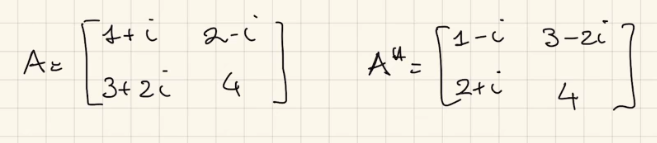
\includegraphics[scale=0.75]{13.png}
\end{center}
%TODO proof of biunivocal representation on the Bloch's sphere.
\begin{list}{}{}
	\item $\theta$ is equivalent to the geometrical latitude: angle with the $z$ axis
	\item $\phi$ is equivalent to the geometrical longitude: angle with the projection on the $(x,y)$ plane and the $x$ axis
\end{list}
\subsubsection{Evolution Postulate}
The time evolution of a closed quantum system is described by the \textbf{Schrodinger Equation} $$ih\frac{d\:|\psi(t)\rangle}{dt} = H(t)\:|\psi(t)\rangle$$
With $h$ being the \textbf{Planck's Constant} and $H(t)$ being the \textbf{fixed Hermitian operator} known as the Hamiltonian of the system.
\paragraph{Notes} The postulate describes the evolution of a quantum system in continuous time, with the change described by a differential equation. The Hamiltonian $H(t)$ represent the \textbf{total energy} function for the system and tells the quantum state how to change.\\
If we know the Hamiltonian of a system, then we understand its dynamics completely (at least in principle). In general, figuring it out is very difficult.
\paragraph{Simplified: Discrete Time Evolution} The discrete time evolution of a closed quantum system is described by a \textbf{unitary transformation}. The state $\ket{\psi}$ of the system at time $t_1$ is related to the state $|\psi'\rangle$ at a later time $t_2$ by a unitary matrix $U$ which depends only on the times $t_1$ and $t_2$ $$|\psi'\rangle = U\ket{\psi}$$
This means applying gates one at the time.
\paragraph{Notes} This expression follows directly form the Schrodinger Equation: every unitary operator $U$ can be realized as a solution of Schrodinger Equation. This postulate, though, doesn't tell us which unitary transformations to use to describe real-world quantum dynamics: case-by-case analysis to figure it out.\\
Unitary matrices because they preserve length.
\paragraph{Measurements} We postulate that closed quantum systems evolve according to a unitary operator. We will be interested in observing and \textbf{measuring} some properties of a system: at some point we must allow the system to interact with the measurement apparatus, making the system no longer closed and the Evolution Postulate no longer appropriate.\\
The evolution of the state of a system during a measurement is not unitary: the third postulate provides a means for describing the effects of measurements on quantum systems.\\
Quantum Systems do get perturbed and modified, and only the probability of observing specific values can be calculated: measurement is a non-deterministic process.
\subsubsection{Measurement Postulate}
Quantum measurements are described by a collection $\{M_m\}$ of measurements operators that satisfy the \textbf{completeness relation} $$\sum_m M_m^+ M_m = I$$
$m$ labels the measurement outcomes that may occur in the experiment. If the state of the quantum system is $\ket{\psi}$ immediately before the measurement, then for each $m$:
\begin{list}{}{}
	\item The probability that result $m$ occurs is given by $$p(m) = \langle\psi|M_m^+M_m\ket{\psi} = \|M_m\:\ket{\psi}\|^2$$
	\item The state of the system after the measurement with outcome $m$ is $$\frac{M_m\:\ket{\psi}}{\sqrt{\langle\psi|M_m^+M_m\ket{\psi}}}$$
\end{list}
\paragraph{Notes} This is only a mathematical formalism for measurements. The state of the system after the measurement is a properly normalized quantum state, and in general it is not a scalar multiple of $\ket{\psi}$: the measurement has modified the state of the system.\\
The denominator vanishes only if $p(m) = 0$, meaning that the result $m$ will never occur.\\
The completeness equation expresses the fact that probabilities sum to one: $$\sum_m p(m) = \sum_m \langle\psi|M_m^+M_m\ket{\psi} = \langle\psi|I\ket{\psi} = \langle\psi\ket{\psi} = 1$$
\paragraph{Example} %TODO
\paragraph{Projective Measurements} For many applications of quantum computation and quantum information we will mostly perform \textbf{projective measurements}, as subset of the possible measurements.\\
Defined in terms of the Hermitian operator: an operator $M$ is Hermitian if it's self-adjoint: $M^+ = M$\\
In physics, Hermitian operators are called observable: \textbf{an observable is a property of a physical system that can be measured} (position, polarization\ldots), and to each physical observable there corresponds an Hermitian operator.\\
All eigenvalues of an observable (so of an Hermitian operator) are real, and the eigenvectors are orthogonal. The \textbf{possible outcomes of a measurement correspond to the eigenvalues of the observable} $M$.\\
Observables can be thought of as questions we can pose to quantum systems: each question admits a set of answers, the eigenvalues of the observable.\\\\Any observable $M$ can be written as its \textbf{spectral decomposition} $$M = \sum_m P_m = \sum_m m|u_m\rangle\langle u_m|$$
\begin{list}{}{}
	\item $m$ are the real eigenvalues of $M$ (outcomes)
	\item $|u_m\rangle$ is the eigenvector associated to $m$
	\item $P_m = |u_m\rangle\langle u_m|$ is the \textbf{projector} onto the eigenspace of $M$ with real eigenvalue $m$
\end{list}
Projectors are operators $P$ which satisfy $P^2 = P$\\
An example is the operator $\ket{0}\langle0|$ $$(\ket{0}\langle0|)^2 = \ket{0}\langle0|\ket{0}\langle0| = \ket{0}\:(\langle0\ket{0})\:\langle0| = \ket{0}\langle0|$$ since $\langle0\ket{0} = 1$
\paragraph{Example} %TODO
\paragraph{Expectation}
$$E_\psi[M] = \langle\psi|M\ket{\psi}$$
\paragraph{Recap on Measurement Postulate} It's a mathematical formalism for measurements. It doesn't tell us what measurement can be done in practice or with what efficiency. Some measurements can be simple to state mathematically but \textbf{not easy to implement}.\\
Tells us how to compute the probability $P(m)$ that outcome $m$ occurs and the new state of the system after the measurement with outcome $m$ applying the measurement operators $M_m$ (one operator for each possible outcome).\\
For projective measurement, these operators, can be derived from the spectral decomposition of the observable $M$ corresponding to the measurement.\\
An observable is a property of a physical system (a \textbf{physical quantity}) that can be measured: position, polarization\ldots Each physical observable corresponds to a \textbf{Hermitian operator}, all eigenvalues of an observable are real and the eigenvectors are orthogonal. The \textbf{possible outcomes of a measurements are the real eigenvalues of $M$}.
Any observable $M$ can be written it as its \textbf{spectral decomposition} $$M = \sum_m mP_m = \sum_m m|u_m\rangle\langle u_m|$$
where \begin{list}{}{}
	\item $m$ are the real eigenvalues, the outcomes of the measurements
	\item $|u_m\rangle$ is the eigenvector associated to $m$
	\item $P_m = |u_m\rangle\langle u_m|$ is the \textbf{projector} onto the eigenspace of $M$ with real eigenvalue $m$
\end{list}
The measurement operators are the projectors $P_m = |u_m\rangle\langle u_m|$\\
The probability of getting result $m$ on the state $\ket{\psi}$ is $$p(m) = \langle\psi\:|\:P_m^+ P_m\:|\:\psi\rangle = \langle\psi|P_m\ket{\psi} $$
Given that outcome $m$ occurred, the state of the quantum system immediately after is $$\frac{P_m\ket{\psi}}{\sqrt{p(m)}}$$
The operators $P_m$ satisfy the completeness relation.
$$\sum_m P_m^+P_m = \sum_m P_m = I$$
\paragraph{Measurements in the Standard Basis} A measurement in the $\ket{0}, \ket{1}$ basis corresponds to perform a projective measurement with projectors $$P_0 = \ket{0}\langle 0| = \left(\begin{array}{c}1//0\end{array}\right) (1\:\:0) = \left(\begin{array}{c c}1&0\\0&0\end{array}\right)$$
$$P_1 = \ket{1}\langle 1| = \left(\begin{array}{c}1//0\end{array}\right) (1\:\:0) = \left(\begin{array}{c c}0&0\\0&1\end{array}\right)$$
Can be seen as projective measurement with respect to Hermitian matrix $Z$
$$Z = \ket{0}\langle 0| - \ket{1}\langle 1| = \left(\begin{array}{c c}
1&0\\0&-1
\end{array}\right)$$
Or also with respect to $I$ with eigenvalues equal to 1
$$I = \ket{0}\langle 0| + \ket{1}\langle 1| = \left(\begin{array}{c c}
1&0\\0&1
\end{array}\right)$$
\paragraph{Measurements in Orthonormal Basis} A measurement in an orthonormal basis $\{|m\rangle\}$ corresponds to perform a projective measurement with projector operators $$P_m=|m\rangle\langle m|$$
For example in the hadamard basis $\ket{+}, \ket{-}$
$$\ket{+} = H\ket{0} = \frac{\ket{0}+\ket{1}}{\sqrt{2}}$$
$$\ket{-} = H\ket{1} = \frac{\ket{0}-\ket{1}}{\sqrt{2}}$$
Corresponds to perform projective measurement with projectors
$$P_+ = \ket{+}\langle +| = \frac{1}{2}\left(\begin{array}{c}
1\\1
\end{array}\right) (1\:1) = \frac{1}{2}\left(\begin{array}{c c}
1&1\\1&1
\end{array}\right)$$
$$P_- = \ket{-}\langle -| = \frac{1}{2}\left(\begin{array}{c}
1\\-1
\end{array}\right) (1\:-1) = \frac{1}{2}\left(\begin{array}{c c}
1&-1\\-1&1
\end{array}\right)$$
And the completeness equation is satisfied $$P_+^+P_+ + P_-^+P_+ = P_+ + P_- = I$$
Single qubit measurements: measuring the identity but also measures the projection over the $x$ axis. All Pauli matrices have eigenvalues of +1 and -1:
$$X = \ket{+}\langle +| - \ket{-}\langle -| = \left(\begin{array}{c c}
0&1\\1&0
\end{array}\right)$$
\subparagraph{Measuring example} Measuring the state $$\ket{\psi} =\alpha\ket{0} + \beta\ket{1}$$
in the $\ket{+},\ket{-}$ basis gives the result $+$ with probability $$P(+) = \langle\psi|P_+\ket{\psi} = \langle\psi\ket{+}\langle+\ket{\psi} = \frac{1}{2}|\alpha + \beta|^2$$ %TODO
and state after the measurement is $\ket{+}$, while it gives the result $-$ with probability $$P(-) = \langle\psi|P_-\ket{\psi} = \langle\psi\ket{-}\langle-\ket{\psi} = \frac{1}{2}|\alpha - \beta|^2$$ %TODO
and state after is $\ket{-}$.\\
Also relative phase factors are important. Consider the state $\ket{+},\ket{-}$ differing just for a relative phase factor (plus and minus)
$$\ket{+} = \frac{1}{\sqrt{2}}(\ket{0} + \ket{1})\:\:\:\:\:\ket{-} = \frac{1}{\sqrt{2}}(\ket{0} - \ket{1})$$
We cannot distinguish between them by measuring in the computational basis: both 0,1 outcomes occur with probability $\frac{1}{2}$.\\
Considering the $\ket{+},\ket{-}$ basis, which has measurements operators $P_+,P_-$ if we measure the state $\ket{+}$ we always get outcome $+$, $P(+) = 1, P(-) = 0$. Opposite for measuring $\ket{-}$ getting always $-$ as outcome. So measuring in the $\ket{+},\ket{-}$ basis distinguish the two state perfectly, relative phase matters.\\
How to measure in a basis different from the computational basis? In the computational basis we have a register, quantum information becomes classical information. How to measure in different basis, for instance the hadamard basis?\\
First we apply a change of basis from the hadamard back to the computational. Then measure respect to the computational and after we change back to the original basis. Example %TODO
We measure either $\ket{0}$ or $\ket{1}$, how to change back? Just apply again the change of basis transformation, since the circuits are always reversible.\\
In general, to implement a measurement with respect to an orthonormal basis $\{\phi_j\rangle\}$:\begin{list}{}{}
	\item The matrix $U$ is applied to perform a basis change to the computational basis
	$$U\left(\sum_j\alpha_j|\phi_j\rangle\right) = \sum_j\alpha_jU|\phi_j\rangle = \sum_j\alpha_j|j\rangle$$
	\item Then a measurement is made in the computational basis obtaining a specific (classical) outcome with probability $|\alpha_j|^2$.\\
	The state of the system after this measurement is $|j\rangle$
	\item Finally $U^{-1}$ is applied to change back to the $\{|\phi_j\rangle\}$ basis, leaving the post-measurement state $|\phi_j\rangle$
\end{list}
\subsubsection{Composition of Systems}
The \textbf{state space of a composite physical system is the tensor product of the state spaces of the component subsystems}. Moreover, if we have systems numbered 1 through $n$, and system number $i$ is prepared in the state $|\psi_i\rangle$, then the joint state of the total system is
$$|\psi_1\rangle\otimes\ldots\otimes|\psi_n\rangle$$
Often $\otimes$ is omitted and the above formula is rewritten as $|\psi_1,\ldots,\psi_n\rangle$\\
Tensor product is the mathematical structure used to describe the state space of a composite physical system because we need a new space which captures the interaction of all $n$ systems.\\
Not all states of acombined system can be separated into the tensor product of states of the individual components.\\
Notation:
\begin{list}{}{}
	\item $\ket{\psi} = \alpha\ket{0}+\beta\ket{1} = \left(\begin{array}{c}
	\alpha\\\beta
	\end{array}\right)$
	\item $\ket{\phi} = \gamma\ket{0}+\delta\ket{1} = \left(\begin{array}{c}
	\gamma\\\delta
	\end{array}\right)$
	\item \textbf{Joint state of the two qubits}
	$$\ket{\psi}\otimes\ket{\phi} = \left(\begin{array}{c}
	\alpha\\\beta
	\end{array}\right)\otimes\left(\begin{array}{c}
	\gamma\\\delta
	\end{array}\right) = \left(\begin{array}{c}
	\alpha\gamma\\\alpha\delta\\\beta\gamma\\\beta\delta
	\end{array}\right) = \alpha\gamma|00\rangle + \alpha\delta|01\rangle + \beta\gamma|10\rangle + \beta\delta|11\rangle$$
	\item \textbf{Standard basis notation}
	$$|00\rangle=\left(\begin{array}{c}1\\0\\0\\0\end{array}\right)\:\:|01\rangle=\left(\begin{array}{c}0\\1\\0\\0\end{array}\right)\:\:|10\rangle=\left(\begin{array}{c}0\\0\\1\\0\end{array}\right)\:\:|11\rangle=\left(\begin{array}{c}0\\0\\0\\1\end{array}\right)$$
\end{list}
\paragraph{Separable States} A state $\ket{\psi}\in C^n\otimes C^m$ of a combined system is a \textbf{separable state} if it can be expressed as $\ket{\psi} = |\psi_1\rangle\otimes|\psi_2\rangle$ for some $|\psi_1\rangle\in C^n$ and $|\psi_2\rangle\in C^m$\\
For example $$\frac{1}{2}(|00\rangle+|01\rangle+|10\rangle+|11\rangle) = \frac{1}{\sqrt{2}}(\ket{0} + \ket{1})\otimes \frac{1}{\sqrt{2}}(\ket{0}+\ket{1})$$
For example we get separable state when qubits are prepared independently and kept isolated.\\
Physical separation does not imply that the joint state must be separable. Two physically separated particles can be entangled (correlated).
\paragraph{Entangled States} A state of a composite system that cannot be written as a product of states of its component systems is called \textbf{entangled state}.\\
For example the bell state is entangled, cannot be writted as a product of single-qubit states:
$$\ket{\psi}=\frac{1}{\sqrt{2}}(|00\rangle+|11\rangle) = \frac{1}{\sqrt{2}}\left(\begin{array}{c}
1\\0\\0\\1
\end{array}\right)$$
%TODO dim
Either $\alpha$ or $\delta$ must be zero but with alpha zero the first element is zero, with delta zero the last element is zero. Cannot exist.
\paragraph{Example} 2 qubit composite system $|\psi_1\rangle\otimes|\psi_2\rangle$ where we apply the $X$ (NOT) gate only to the first qubit. So implicitly we apply the identity gate $I$ to the second qubit.
$$|\psi_1\rangle\otimes|\psi_2\rangle\mapsto X|\psi_1\rangle\otimes I|\psi_2\rangle = (X\otimes I)(|\psi_1\rangle\otimes|\psi_2\rangle)$$
So for a $n$ qubit composite system $|\psi_1\rangle\otimes\ldots\otimes|\psi_n\rangle$, applying the $X$ gate to the first qubit corresponds to applying the operation $X\otimes I\otimes\ldots\otimes I$ (with $I$ repeated $n-1$ times) to the entire system.
\paragraph{CNOT Gate} Just as there are 2-qubit states that cannot be written as the product of two 1-qubit states, there are 2-qubit gates (acting on both qubits) that cannot be written as a tensor product of two 1-qubit gates.\\
The CNOT gate flips the state of the second qubit if the first qubit is in state $\ket{1}$, and does nothing otherwise:
$$|00\rangle\mapsto|00\rangle$$
$$|01\rangle\mapsto|01\rangle$$
$$|10\rangle\mapsto|11\rangle$$
$$|11\rangle\mapsto|10\rangle$$
Represented as a matrix:
$$\left(\begin{array}{c c c c}
1&0&0&0\\
0&1&0&0\\
0&0&0&1\\
0&0&1&0
\end{array}\right)$$
and \textbf{cannot be written as a tensor product of two 1-qubit gates}.
\paragraph{Measurements on Multiple Qubits} Considering a two qubit state
$$\ket{\psi}=\alpha|00\rangle+\beta|01\rangle+\gamma|10\rangle+\delta|11\rangle$$
a complete set of measurement operators in the computational basis would be 
$$P_{00} = |00\rangle\langle00\rangle\:\:P_{01} = |01\rangle\langle01\rangle\:\:P_{10} = |10\rangle\langle10\rangle\:\:P_{11} = |11\rangle\langle11\rangle$$
When measuring the two qubits we get\begin{list}{}{}
	\item the result $00$ with probability $|\alpha|^2$
	\item the result $01$ with probability $|\beta|^2$
	\item the result $10$ with probability $|\gamma|^2$
	\item the result $11$ with probability $|\delta|^2$
\end{list}
How do we measure only the first qubit? We \textbf{tensor the desired measurement operator with the identity matrix}: if we measure the first qubit to be in state $\ket{0}$, the measurement operator will consist of projectors onto the state $|00\rangle,|01\rangle$ since we must consider all states consistent with the measurements.
$$P_{0*} = |00\rangle\langle00| + |01\rangle\langle01| = (\ket{0}\otimes\ket{0})(\langle0|\otimes\langle0|) + (\ket{0}\otimes\ket{1})(\langle0|\otimes\langle1|) =$$
$$=\ket{0}\langle0|\otimes\ket{0}\langle0|+\ket{0}\langle0|\otimes\ket{1}\langle1| = \ket{0}\langle0|\otimes(\ket{0}\langle0|+\ket{1}\langle1|) = \ket{0}\langle0|\otimes I$$
because $(A\otimes B)(C\otimes D) = (AC)\otimes(BD)$. Similarly
$$P_{1*} = |10\rangle\langle10|+|11\rangle\langle11| = \ldots = \ket{1}\langle1|\otimes I$$
\pagebreak

Therefore the probability of measuring the first qubit in state $\ket{0}$ is $$p(0) = \langle\psi|P_{0*}\ket{\psi} = \langle\psi|\:\ket{0}\langle0|\otimes I\ket{\psi} = (\alpha*\:\beta*\:\gamma*\:\delta*)\left(\begin{array}{c c c c}
1&0&0&0\\
0&1&0&0\\
0&0&0&0\\
0&0&0&0
\end{array}\right)\left(\begin{array}{c}
\alpha\\\beta\\\gamma\\\delta
\end{array}\right) =(\alpha*\:\beta*\:\gamma*\:\delta*)\left(\begin{array}{c}
\alpha\\\beta\\0\\0
\end{array}\right) = |\alpha|^2+|\beta|^2$$
As expected $p(0)$ is the sum of the probabilities of measuring $|00\rangle$ and $|01\rangle$.\\
The state after the measurement is 
$$\frac{P_{0*}\ket{\psi}}{\sqrt{p(0)}} = \frac{1}{\sqrt{|\alpha|^2+|\beta|^2}} (\ket{0}\langle0|\otimes I)(\alpha|00\rangle + \beta|01\rangle + \gamma|10\rangle + \delta|11\rangle) = \frac{1}{\sqrt{|\alpha|^2+|\beta|^2}}(\alpha|00\rangle+\beta|01\rangle)$$
The relative probability of observing $|00\rangle$ and $|01\rangle$ hasn't changed, but by measuring $\ket{0}$ on the first qubit we have eliminated the possibilities that the system is in either the state $|10\rangle$ or $|11\rangle$
\paragraph{Example} Given $$\ket{\psi}=\sqrt{\frac{1}{11}}|00\rangle+\sqrt{\frac{5}{11}}|01\rangle+\sqrt{\frac{2}{11}}|10\rangle+\sqrt{\frac{3}{11}}|11\rangle$$
Then the probability of measuring $0$ in the first qubit is $\frac{1 + 5}{11} = \frac{6}{11}$ and the state after measuring it becomes
$$\sqrt{\frac{11}{6}}\left(\sqrt{\frac{1}{11}}|00\rangle+\sqrt{\frac{5}{11}}|01\rangle\right)$$
\subsection{Superdense Coding}
Simple yet surprising application of elementary quantum mechanics. It involves two parties, Alice and Bob, who are far away from each other and the goal is the following: Alice in in possession of two classical bits of information which she wishes to send to Bob \textbf{using a single qubit}.\\
Alice and Bob initially share a pair of qubits in the entangled Bell state $$|\beta_{00}\rangle = \frac{|00\rangle + |11\rangle}{\sqrt{2}}$$
One qubit is in Alice's possession, the other is in Bob's possession.\\
How are the Bell states formed?
\begin{center}
	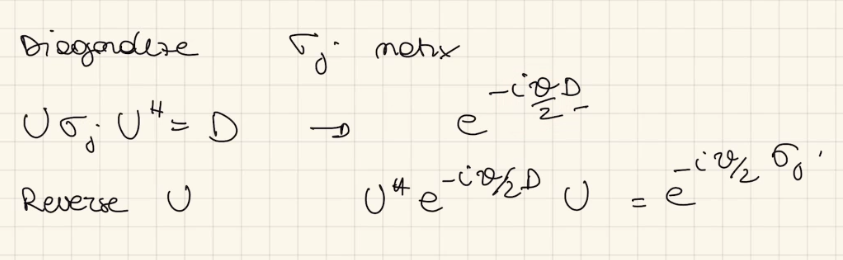
\includegraphics[scale=0.5]{15.png}
\end{center}
$$|00\rangle \rightarrow H\otimes I\rightarrow \frac{\ket{0}+\ket{1}}{\sqrt{2}}\ket{0}\rightarrow\hbox{CNOT}\rightarrow\frac{|00\rangle+|11\rangle}{\sqrt{2}} = |\beta_{00}\rangle$$
$$|01\rangle \rightarrow H\otimes I\rightarrow \frac{\ket{0}+\ket{1}}{\sqrt{2}}\ket{1}\rightarrow\hbox{CNOT}\rightarrow\frac{|01\rangle+|10\rangle}{\sqrt{2}} = |\beta_{01}\rangle$$
$$|10\rangle \rightarrow H\otimes I\rightarrow \frac{\ket{0}-\ket{1}}{\sqrt{2}}\ket{0}\rightarrow\hbox{CNOT}\rightarrow\frac{|00\rangle-|11\rangle}{\sqrt{2}} = |\beta_{10}\rangle$$
$$|11\rangle \rightarrow H\otimes I\rightarrow \frac{\ket{0}-\ket{1}}{\sqrt{2}}\ket{1}\rightarrow\hbox{CNOT}\rightarrow\frac{|01\rangle-|10\rangle}{\sqrt{2}} = |\beta_{11}\rangle$$
\textbf{Every vector is this basis is entangled!}
\paragraph{Sharing a Pair of Entangled Bits}\begin{list}{}{}
	\item The state $|\beta_{00}\rangle$ would have to be created ahead of time, when the qubits are in a lab together and can be made to interact in a way that will give rise to the entanglement between them.
	\item After the state is created, Alice and Bob each take one of the two qubits away with them.
\end{list}
Alternatively, some third party may prepare the entangled state ahead of time and sens one qubit to Alice and the other to Bob.\\\\
If they are careful not to let the qubits interact with the environment or other quantum systems, Alice and Bob's joint state will remain entangled.\\
Note that $|\beta_{00}\rangle$ is a fixed state, there is no need for Alice to have sent any qubit to Bob to prepare this state.
\begin{center}
	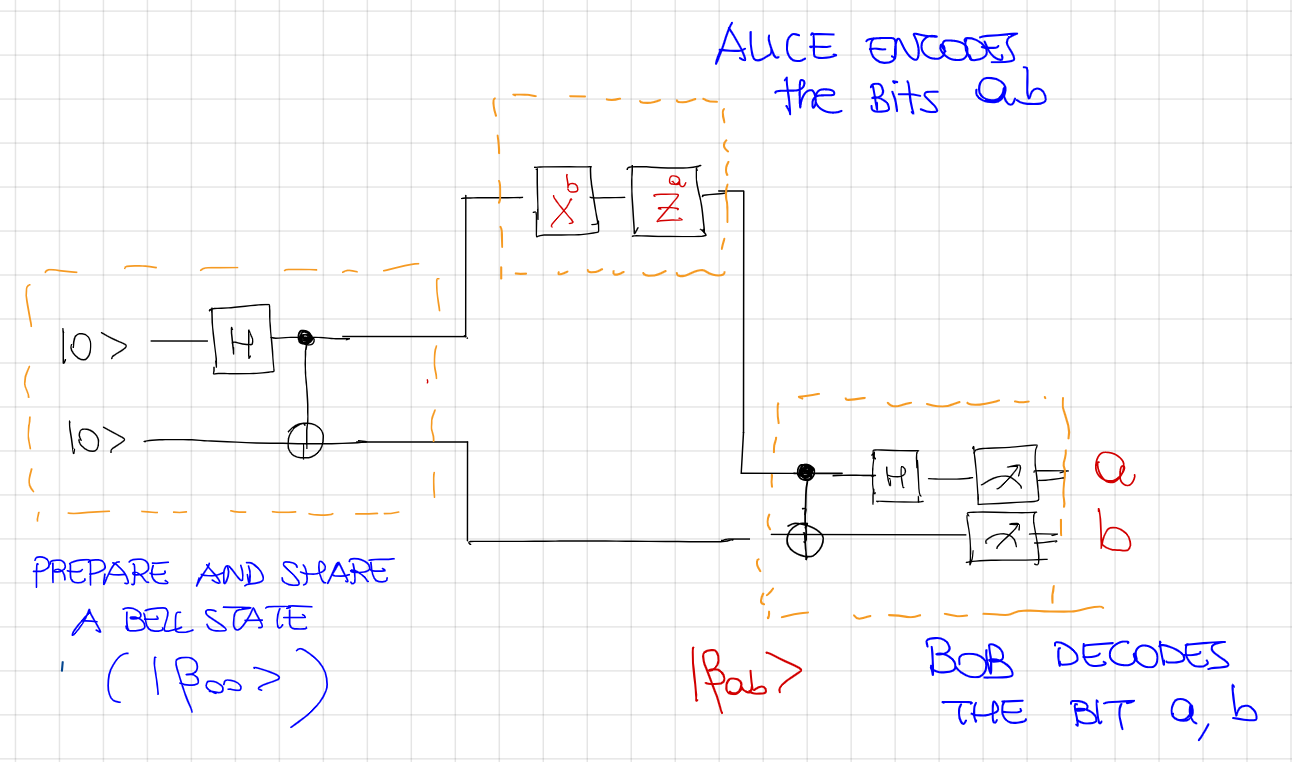
\includegraphics[scale=0.5]{16.png}
\end{center}
\paragraph{Procedure}
\begin{center}
	\begin{tabular}{c c l}
\textbf{To send}&\makecell{\textbf{Alice applies to her}\\\textbf{qubit the gate}}&\textbf{Resulting state}\\
\hline
00&$I$& $|\beta_{00}\rangle \mapsto |\beta_{00}\rangle$ \\
01&$X$& $|\beta_{00}\rangle \mapsto \frac{|10\rangle+|01\rangle}{\sqrt{2}} = |\beta_{01}\rangle$\\
10&$Z$& $|\beta_{00}\rangle \mapsto  \frac{|00\rangle-|11\rangle}{\sqrt{2}} = |\beta_{10}\rangle$\\
11&$ZX$& \makecell{$|\beta_{00}\rangle \mapsto_{X\otimes I}\frac{|10\rangle+|01\rangle}{\sqrt{2}}\mapsto_{Z\otimes I}\frac{-|10\rangle+|01\rangle}{\sqrt{2}}=|\beta_{11}\rangle$}
\end{tabular}
\end{center}
The resulting state is one of the four Bell states, which form an orthonormal basis and can be distinguished by an appropriate quantum measurement. So after applying the appropriate gate, Alice sends her qubit to Bob. Bob is in possession of one of the four Bell states, depending on the classical bits that Alice wished to send him, so he performs a measurement in the Bell basis and determines which bit string Alice sent.\\
The measurement can be implemented by first performing a change of basis, then performing a measurement in the computational basis.\\
The outcome of the Bell measurement reveals to Bob the Bell states he possesses and allows him to determine with certainty the two classical bits.\\
The measurement gives Bob the values $a,b$ corresponding to the Bell state $|\beta_{ab}\rangle$ in his possession.
\paragraph{Example} Alice wants to send $10$, so she applies $Z$ to her qubit
$$|\beta_{00}\rangle = \frac{|00\rangle+|11\rangle}{\sqrt{2}} \mapsto_{Z\otimes I}\frac{|00\rangle-|11\rangle}{\sqrt{2}}$$
and send the qubit to Bob. Bob performs the measurement: applies a CNOT with the first qubit as control and the second as target, then a Hadamard on the first:
$$\frac{|00\rangle-|11\rangle}{\sqrt{2}} \mapsto_{\hbox{CNOT}}\frac{|00\rangle-|10\rangle}{\sqrt{2}}\mapsto_{H\otimes I}\frac{1}{\sqrt{2}}\left(\frac{\ket{0}+\ket{1}}{\sqrt{2}}\ket{0}-\frac{\ket{0}-\ket{1}}{\sqrt{2}}\ket{0}\right)=$$
$$=\frac{1}{2}(\cancel{|00\rangle}+|10\rangle \cancel{-|00\rangle}+|10\rangle) = \frac{1}{2}(2|10\rangle) = |10\rangle$$
Now Bob has the state $|10\rangle$ and know that Alice sent $10$.\\\\
Alice, interacting with only a single qubit, is able to transmit two bits of information to Bob. Two qubits are involved in the protocol, but Alice never need to interact with the second qubit. Classically, the task Alice accomplishes would have been impossible had she only transmitted a single classical bit.\\
Information is physical, and surprising physical theories as Quantum Mechanics may predict surprising information processing abilities.
\paragraph{Communication Channels}
\begin{list}{}{}
	\item \textbf{Quantum Communication Channel} is a communication line (e.g. fiber optic, cable\ldots) which can carry qubits between two remote locations.
	\item \textbf{Communication Channel} is a line that can carry only classical bits (and not qubits).
\end{list}
\paragraph{Quantum Teleportation} Process by which a quantum state is transfered from one location to another, without sending directly the quantum state.\\
Alice has $\ket{\psi} = \alpha\ket{0}+\beta\ket{1}$ and would like to send the quantum state to Bob.\begin{list}{}{}
	\item Alice could physically send the qubit but we rule out this possibility because we want to "teleport".
	\item Alice could tell Bob the amplitude $\alpha$ and $\beta$ for the quantum state $\ket{\psi}$. To do this, she doesn't need to send a quantum state, but she can simply send the complex numbers $\alpha$ and $\beta$ as ordinary classical information e.g. over the internet. Bob could then re-create the state in his lab.\\
	But \textbf{in general Alice doesn't know the identity of her quantum state}.
\end{list}
\textbf{Quantum teleportation works even when the identity of a the state isn't known to Alice or Bob}.
The teleportation instead works like this. The circuit is:
\begin{center}
	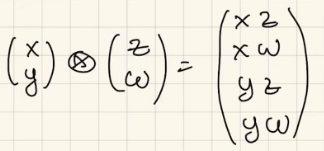
\includegraphics[scale=0.5]{17.png}
\end{center}
Alice has two qubits, Bob just one.
\begin{list}{}{}
	\item \textbf{Step 1}: two qubits are prepared entangled and shared.
	\item \textbf{Step 2}: Alice lets the two qubits interact and measure with a Bell basis measurement, basically by changing the base.
	\item \textbf{Step 3}: Alice measures her two qubits in the computational basis. She has 4 possible equiprobable outcomes.
	\item \textbf{Step 4}: Bob receives the two classical bits from Alice and restores the state $\ket{\psi}$ on his qubit.
\end{list}
No particle have been sent from Alice to Bob, just two classical bits used by Bob to recover the state $\ket{\psi}$. Moving is possible, copying is not possible: $\ket{\psi}$ is not in possession of Alice anymore.\\
Alice measures in the Bell state because: after step one we have $\ket{\psi}|\beta_{00}\rangle$ and you can prove that this is equal to $$\ket{\psi}|\beta_{00}\rangle = \frac{1}{2}(|\beta_{00}\rangle\ket{\psi} + |\beta_{01}\rangle X\ket{\psi} + |\beta_{10}\rangle Z\ket{\psi} + |\beta_{11}\rangle XZ\ket{\psi})$$
\section{Quantum Algorithms}
The really important question is when quantum computers can outperform classical ones.\\
With a $$f:\{0,1\}\rightarrow\{0,1\}$$ we have 4 functions
\begin{center}
	\begin{tabular}{c | c c c c}
& $f_1$ & $f_2$ & $f_3$ & $f_4$\\
\hline
0 & 0 & 0 & 1 & 1\\
1 & 0 & 1 & 0 & 1
\end{tabular}
\end{center}
With classical algorithms we need two queries to see if a function is balanced or constant. In quantum algorithms we need to query the oracle only once because we can exploit quantum parallelism. Feed the circuit with a superposition of inputs and the oracle returns a superposition of outputs. This is the \textbf{Deutsch algorithm}, and the \textbf{Deutsch problem} is the following: given a black box for computing an unknown function $f:\{0,1\}\rightarrow\{0,1\}$, determine if the function is balanced or constant by making queries to $f$.
\subsection{Classical Computations on Quantum Computers}
We want to compute functions $$f:\{0,1\}^n\rightarrow\{0,1\}$$ We need to have a \textbf{reversible computation}, so unitary gates: can't feed the entire input sequence into a gate. We take any classical logic circuits computing out function, than change each gate into a reversible version. Once we have a computable function with reversible gate than we can translate it into a quantum ambient.\\
To translate a gate into a reversible version we use Toffoli gates, which are reversible versions of the AND. Toffoli gates are C-CNOT. With $C= 0$ is AND, with $C=1$ is a NAND.\\
Toffoli gate and the quantum implementation:
\begin{center}
	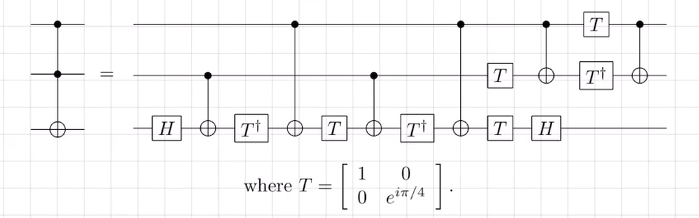
\includegraphics[scale=0.5]{19.png}
\end{center}
Any classical computation can be implemented by a quantum circuit of Toffoli gates.
\paragraph{Quantum Parallelism} An oracle computing a function is a black-box that computes said function. Quantum if used with quantum bits.\\
$U_f$ is implemented, due to reversibility, with input $\ket{x}$ of size $n$ and another qubit $|y\rangle$ used to store the result. The output is $\ket{x}$ and $|y\otimes f(x)\rangle$. It's reversible
$$|x,y\rangle\mapsto_{U_f} |x,y\otimes f(x)\rangle \mapsto_{U_f} |x, (y\otimes f(x))\otimes f(x) \rangle = |x,y\rangle$$
In general $\ket{x}$ is of size $n$, meaning $f:\{0,1\}^n\rightarrow\{0,1\}$. To prepare the $\ket{x}$ (data register) in a superposition we apply the Hadamard gate, and we can generalize this procedure on an arbitrary number of qubits:\begin{center}
	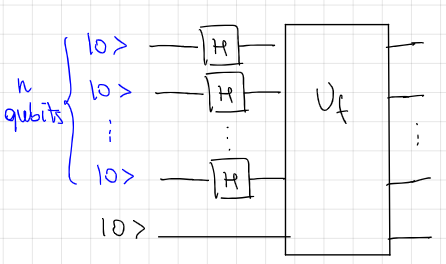
\includegraphics[scale=0.5]{20.png}
\end{center}
So we:\begin{list}{}{}
	\item Prepare the $n+1$ qubit state $\ket{x}^{\otimes n}|y\rangle$
	\item Apply the $H$ gate to the first $n$ qubits, to obtain the equal superposition of all inputs of $f$
	\item Apply the quantum circuit implementing $U_f$
\end{list}
Obtaining the state $\frac{1}{\sqrt{2^n}}\sum_x|x,f(x)\rangle$\\
Quantum parallelism enables all possible values of $f$ to be evaluated simultaneously, even if we evaluate $f$ once. This parallelism is not immediately useful: if we measure the state $\frac{1}{\sqrt{2^n}}\sum_x|x,f(x)\rangle$ we obatin $|x,f(x)\rangle$ for a single value of $x$.\\
To exploit quantum parallelism, we need the ability to extract information about more than one value of $f(x)$ from $\sum_x |x,f(x)\rangle$
\subsection{Deutsch's Algorithm}
\begin{center}
	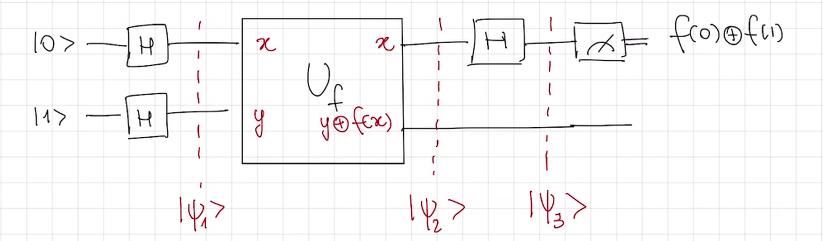
\includegraphics[scale=0.5]{22.png}
\end{center}
$$f(0)\otimes f(1)=\left\{\begin{array}{c l}
0 & f\hbox{ is constant}\\
1 & f\hbox{ is balanced}
\end{array}\right.$$
This circuit solves Deutsch's problem in just one pass. The Hadamard gate on the state $\ket{1}$ is to let the amplitude interfere in order to grasp global properties of the function. The last part measures in the Hadamard basis.
$$|\psi_1\rangle = \ket{+}\ket{-} = \frac{\ket{0}+\ket{1}}{\sqrt{2}}\frac{\ket{0}-\ket{1}}{\sqrt{2}} = \frac{1}{\sqrt{2}}\ket{0}\ket{-} + \frac{1}{\sqrt{2}}\ket{1}\ket{-}$$
Recall that the oracle $U_f$ works like this\begin{list}{}{}
	\item $\ket{x}\ket{-} = \ket{x}\frac{\ket{0}-\ket{1}}{\sqrt{2}} \mapsto_{U_f} \ket{x}\frac{|0\oplus f(x)\rangle - |1\otimes f(x)\rangle}{\sqrt{2}} = \ket{x}\frac{|f(x)\rangle - |\overline{f(x)}\rangle}{\sqrt{2}} = \left\{\begin{array}{l l}
	\ket{x}\frac{\ket{0}-\ket{1}}{\sqrt{2}} = \ket{x}\ket{-} & f(x) = 0\\
	\ket{x}\frac{\ket{1}-\ket{0}}{\sqrt{2}} = -\ket{x}\ket{-} & f(x) = 1
\end{array}	 \right.$\\
	With $\overline{x}$ being the complement of $x$ (if $x=0$ then $\overline{x} = 1$)\\
	So the state doesn't change with $f(x) = 0$ and has a phase factor with $f(x) = 1$. A more compact way is $(-1)^{f(x)}\ket{x}\ket{-}$
\end{list}
So we have $$|\psi_2\rangle = U_f(\ket{+}\ket{-}) = U_f\left(\frac{\ket{0}\ket{-}}{\sqrt{2}}+\frac{\ket{1}\ket{-}}{\sqrt{2}}\right) = \frac{(-1)^{f(0)}\ket{0}\ket{-} + (-1)^{f(1)}\ket{1}\ket{-}}{\sqrt{2}} = \frac{(-1)^{f(0)}\ket{0} + (-1)^{f(1)}\ket{1}}{\sqrt{2}}\ket{-} =$$
$$=\left\{\begin{array}{l l}
\pm\frac{\ket{0}+\ket{1}}{\sqrt{2}}\ket{-} = \pm\ket{+}\ket{-} & f\hbox{ is constant and }f= 0\hbox{ or }1\\
\pm\frac{\ket{0}-\ket{1}}{\sqrt{2}}\ket{-} = \pm\ket{-}\ket{-} & f\hbox{ is balanced and }f(0) = 0, f(1) = 1\hbox{ or viceversa}
\end{array}\right. $$
Then we apply Hadamard on the first qubit
$$|\psi_3\rangle = (H\otimes I)|\psi_2\rangle = \left\{\begin{array}{l l}
\pm (H\ket{+})\ket{-}& f\hbox{ is constant}\\
\pm (H\ket{-})\ket{-}& f\hbox{ is balanced}
\end{array}\right. = \left\{\begin{array}{l l}
\pm \ket{0}\ket{-}& f\hbox{ is constant}\\
\pm \ket{1}\ket{-}& f\hbox{ is balanced}
\end{array}\right.$$
With a measure on the computational basis we solve the Deutsch's problem, getting 0 $\Leftrightarrow f$ is constant and $1\Leftrightarrow f$ is balanced.
\subsection{Deutsch-Jozsa Algorithm} Generalization of the Deutsch's problem
$$f:\{0,1\}^n\rightarrow\{0,1\}$$
As input we have a black box for computing an unknown function $f:\{0,1\}^n\rightarrow\{0,1\}$ either constant or balanced.\\
The problem is to determine whether $f$ is constant or balanced.\\\\
Classical (exact) solution, in the best case we query twice getting two different answers, then $f$ is balanced for sure. The worst case is $2^{n-1}$ queries with the same result, so $2^{n-1}+1$ queries: if the last value is different then is balanced, otherwise is constant. So classically we need an exponential number of queries. With quantum circuits we do just one query.
\begin{center}
	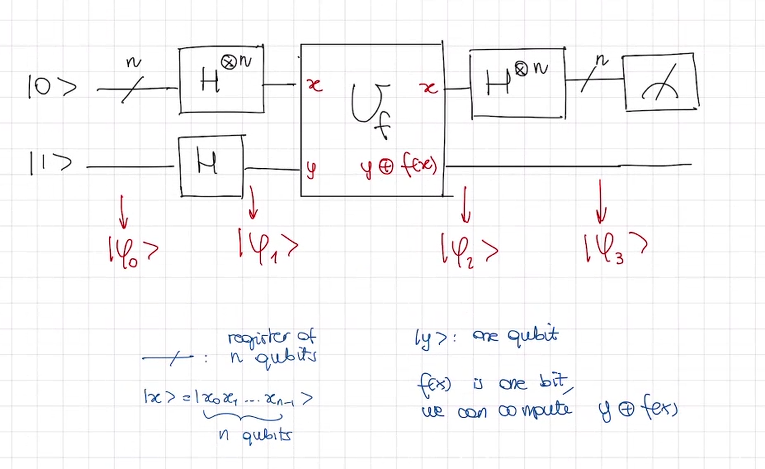
\includegraphics[scale=0.5]{23.png}
\end{center}
Very similar, just with a $n$ qubits on state $\ket{0}$ in the query register and 1 qubit in state $\ket{1}$ in the answer register.
$$|\psi_0\rangle = |0\ldots 0\rangle\ket{1} = \ket{0}^{\otimes n}\ket{1}$$
$$|\psi_1\rangle = \sum_{x\in\{0,1\}^n}\frac{\ket{x}}{\sqrt{2}}\ket{-}$$
Query register: uniform superposition of all values.\\
Answer register: uniform superposition of state $\ket{0}$ and $\ket{1}$.
$$|\psi_2\rangle = \frac{1}{\sqrt{2^n}}U_f\left(\sum_{x\in\{0,1\}^n}\ket{x}\ket{-}\right) = \frac{1}{\sqrt{2^n}} \sum_{x\in\{0,1\}^n} U_f(\ket{x}\ket{-}) = \frac{1}{\sqrt{2^n}} \sum_{x\in\{0,1\}^n} (-1)^{f(x)}\ket{x}\ket{-}$$
Let's see on a single qubit
$$H|x_i\rangle = \frac{\ket{0}+(-1)^{x_i}\ket{1}}{\sqrt{2}} = \frac{1}{\sqrt{2}} \sum_{z_i\in\{0,1\}} (-1)^{x_i}|z_1\rangle=\left\{\begin{array}{l l}
\frac{1}{\sqrt{2}}\frac{\ket{0}+\ket{1}}{\sqrt{2}} & x_i = 0\\
\frac{1}{\sqrt{2}}\frac{\ket{0}-\ket{1}}{\sqrt{2}} & x_i = 1\\
\end{array}\right.$$
So we have
$$H^{\otimes n}\ket{x} = (H|x_0\rangle)\ldots(H|x_{n-1}\rangle) = \frac{1}{\sqrt{2}}\left(\sum_{z_0=0}^1(-1)^{x_0z_0}|z_0\rangle\right)\ldots\left(\sum_{z_{n-1}=0}^1(-1)^{x_{n-1}z_{n-1}}|z_{n-1}\rangle\right)=$$
$$=\frac{1}{\sqrt{2^n}} \sum_{z_0=0}^1\ldots\sum_{z_{n-1}=0}^1 (-1)^{x_0z_0+\ldots+x_{n-1}z_{n-1}}|z_0\rangle\ldots|z_{n-1}\rangle = \frac{1}{\sqrt{2^n}}\sum_{z\in\{0,1\}^n} (-1)^{x\cdot z}\ket{z}$$
So
$$|\psi_3\rangle = H^{\otimes n}\left(\frac{1}{\sqrt{2^n}}\sum_x(-1)^{f(x)}\ket{x} \right)\ket{-} = \frac{1}{\sqrt{2^n}}\left(\sum_x (-1)^{f(x)}H^{\otimes n}\ket{x}\right)\ket{-} =$$ $$= \frac{1}{\sqrt{2^n}}\left( \sum_x (-1)^{f(x)}\frac{1}{\sqrt{2^n}}\sum_{z\in\{0,1\}^n}(-1)^{x\cdot z}\ket{z}\right)\ket{-} = \frac{1}{2^n}\sum_{z\in\{0,1\}^n}\left(\sum_{x\in\{0,1\}^n}(-1)^{f(x)+x\cdot z}\ket{z}\right)\ket{-}$$
Let's consider the amplitude of the state $\ket{z} = |0\ldots 0\rangle$
$$\frac{1}{2^n}\sum_{x\in\{0,1\}^n}(-1)^{f(x)+0} = \frac{1}{2^n}\sum_{x\in\{0,1\}^n}(-1)^{f(x)}=\left\{\begin{array}{l l}
-1&f\hbox{ is constant and }=0\\
+1&f\hbox{ is constant and }=1\\
0&f\hbox{ is balanced}\\
\end{array}\right.$$
So if $f$ is constant, the amplitude of $|0\ldots0\rangle$ is $\pm 1$ (all other amplitudes are 0 since $|\psi_3\rangle$ is a unit vector), and a measurement in the computational basis is certain to return all zeroes (the binary string 0\ldots 0).\\
If $f$ is balanced, positive and negative contributes cancel each other and the overall amplitude is 0, the measurement is certain not to return all zeroes.
\paragraph{Probability Error} $$2\left(\frac{1}{2}\right)^k = \frac{1}{2^{k-1}}$$
\paragraph{Simon's Algorithm} $$f:\{0,1\}^n\rightarrow\{0,1\}^n$$
Is $f$ one-to-one (bijection) or two-to-one function?
\subsection{Quantum Fourier Transform}
Building block for many important algorithms: QPE, QAA, Shor's, QS\ldots
\paragraph{Discrete Fourier Transform} DFT, essentially multiplying a unitary matrix by a vector. With Fast Fourier Transform we do it in $O(N\log N)$ with $N = 2^n$.\\
We have $x_0,\ldots,x_{N-1}$ and $y_0,\ldots,y_{N-1}$ 
Primitive root of unity $\omega_N = e^{\frac{2\pi i}{N}}$
$$y_N = \frac{1}{\sqrt{N}} = \sum_{j=0}^{N-1} e^{\frac{2\pi ijk}{N}}x_j= \sum_{j=0}^{N-1} \omega_N^{jk}x_j$$
So we have $$y = F_N x$$ with $F_N$ unitary matrix, given by the $k$ indexes. $k=0$ we have all ones in the first row.
$$F_n = \frac{1}{\sqrt{N}}\left[\begin{array}{c c c c}
1 & \ldots & \ldots & 1\\
1 & w_N & \ldots & \omega_N^{N-1}\\
\vdots\\
1
\end{array}\right]$$
$$w_N^{kj}\hbox{ in positions }k,j=0,\ldots,N-1$$
The conjugation of $w_N^{jk}$ is $\cos \pm i\sin$ changing the sign.
$$F_N\cdot F_N^H = \frac{1}{N}\left[\begin{array}{c}
w_{kj}
\end{array}\right]\left[\begin{array}{c}
w_{sp}^{-1}
\end{array}\right] = $$
$F_N$ needs to be unitary so this multiplication must be $I$, so $(F_N\cdot F_N^H)_{st}=\left\{\begin{array}{l l}
0&s\neq t\\
1&s = t
\end{array}\right.$\\
It's provable that $\sum_{j=0}^{N-1}\omega_N^{kj}=\left\{\begin{array}{l l}
N&k= 0\hbox{ mod }N\\
0&k\neq 0\hbox{ mod }N
\end{array}\right.$\\
So essentially we have $$(F_NF_N^H)_{st} = \frac{1}{N}\sum_{j=0}\omega_N^{js}\omega_N^{-jt}= \frac{1}{N}\sum_{j=0}^{N-1}\omega_N^{j(s-t)}$$
So it's unitary %TODO proof
\subparagraph{Example} $n=1, N=2$ $$F_2=\frac{1}{\sqrt{2}}\left[\begin{array}{c c}
1&1\\1&-1
\end{array}\right] = H$$
$$\omega_2 = \cos\pi + i\sin\pi$$
\paragraph{Quantum Fourier Transform} We're in the quantum world, so we're working with quantum states. When we measure we collapse from a state, losing the superposition.\\
$|y\rangle = H^{\otimes n}\ket{x}$ is already a quantum Fourier transform, over a group $Z_2\otimes Z_2\otimes\ldots\otimes Z_2$, binary.\\
Thanks to Coppersmith in 1994, we pass from $O(N\log N) = O(2^n n)$ of the fast (classical) Fourier transform to the $O(n^2)$ of the quantum one, so from exponential to polynomial: an exponential speedup. But they don't compute the same quantities.\\\\
We define QFT on an orthonormal basis $$\ket{0},\ket{1}\ldots|N-1\rangle$$
$$|\tilde{j}\rangle = QFT(|j\rangle)$$
More in general, with $$x=\sum_{j=0}^{N-1} x_j|j\rangle$$ $$|\tilde{x}\rangle = QFT(\ket{x})$$
To define, we start from the classical definition applying to each element of the basis
$$|\tilde{j}\rangle = QFT(|j\rangle) = \frac{1}{\sqrt{N}}\sum_{k=0}^{N-1} e^{\frac{2\pi ijk}{N}}|k\rangle$$
So QFT transforms from the canonical $Z$ basis (computational basis) to the Fourier basis.
\subparagraph{Example} $n=1$, 1-qubit
$$|\tilde{0}\rangle=\frac{1}{\sqrt{2}}(\ket{0}+\ket{1})\:\:\:\:\:|\tilde{1}\rangle=\frac{1}{\sqrt{2}}(\ket{0}-\ket{1})$$
$$|\tilde{j}\rangle=\frac{1}{\sqrt{2}}(\ket{0}+e^{\pi ij}\ket{1})$$
\subparagraph{$N$-qubits System}
With 1-qubit, $\{\ket{0},\ket{1}\}$.\\
With 2-qubit $\{\ket{0},\ket{1},|2\rangle,|3\rangle\}$ which is a short-hand writing of $\{|00\rangle,|01\rangle,|10\rangle,|11\rangle\}$.\\
With $N$-qubits we have the basis $\{\ket{0},\ket{1},\ldots,|N-1\rangle\}$ keeping in mind that it's a short-hand writing, $2^n$ basis states so $2^n$ configuration of bits.\\E.g. $|4\rangle = |100\rangle$\\\\
For $n=3$ $$|\tilde{j}\rangle = \frac{1}{\sqrt{2^3}}\sum_{k=0}^{2^3-1}e^{\frac{2\pi ijk}{2^3}}|k\rangle$$
Remembering that
$$|k\rangle=|k_1k_2k_3\rangle$$
So the sum must be interpreted as $$\sum_k = \sum_{k_1=0}^1\sum_{k_2=0}^1\sum_{k_3=0}^1$$
In the general case
$$|\tilde{j}\rangle = \frac{1}{\sqrt{N}}\sum_{k=0}^{N-1}e^{\frac{2\pi ijk}{2^n}}|k\rangle =$$
with $k=k_1k_2\ldots k_n$ which are digits of the binary representation, so can be rewritten in decimal representation as $k = \sum_{s=1}^n k_s2^{n-s}$
$$= \frac{1}{\sqrt{N}}\sum_{k=0}^{N-1}e^{2\pi ij\sum_{s=1}^n k_s2^{-s}}|k_1\ldots k_n\rangle =$$
$$=\frac{1}{\sqrt{N}}\sum_{k=0}^{N-1}\prod_{s=1}^n e^{\frac{2\pi ij k_s}{2^s}}|k_1\ldots k_n\rangle =$$
If you isolate the first qubit you get a tensor product because of the $\prod$, and the $sum_k$ decomposes into the sums $\sum_{k_1}\sum_{k_2}\ldots$
$$=\frac{1}{\sqrt{N}}\left(\ket{0}+e^{\frac{2\pi ij}{2^1}}\ket{1} \right)\otimes\left(\ket{0}+e^{\frac{2\pi ij}{2^2}}\ket{1} \right)\otimes \ldots\otimes \left(\ket{0}+e^{\frac{2\pi ij}{2^n}}\ket{1} \right)$$
Each qubit has been transformed into something very similar to an Hadamard gate, except for the exponent of $e$.\\
So we went from $$|j\rangle = |j_1\ldots j_n\rangle = |j_1\rangle\otimes\ldots\otimes|j_n\rangle$$ to $$|\tilde{j}\rangle=\frac{1}{\sqrt{N}}\left(\ket{0} + e^{\frac{2\pi ij}{2^1}}\ket{1}\right)\otimes\ldots\otimes\left(\ket{0} + e^{\frac{2\pi ij}{2^n}}\ket{1}\right)$$
with a 1 to 1 correspondence between bits.
$$|j_s\rangle\mapsto|\tilde{j}_s\rangle=\left(\ket{0} +e^{\frac{2\pi ij}{2^s}}\ket{1}\right)$$
Each gets a bit of information from each configuration, with $s$ affecting the relative phase.
\begin{list}{}{}
	\item $\frac{1}{\sqrt{N}} e^{\frac{2\pi i j}{2}} \rightarrow |10\ldots0\rangle$
	\item $\frac{1}{\sqrt{N}} e^{\frac{2\pi i j}{2^n}} \rightarrow |0\ldots01\rangle$
	\item $\frac{1}{\sqrt{N}} e^{\frac{2\pi i j}{2^s}} \rightarrow |0\ldots010\ldots0\rangle$
	\item $\frac{1}{\sqrt{N}} \left(e^{\frac{2\pi i j}{2}} +\ldots+e^{\frac{2\pi i j}{2^n}}\right) = \frac{1}{\sqrt{N}}e^{2\pi i(\frac{j}{2}+\ldots +\frac{j}{2^n})} \rightarrow |1\ldots1\rangle$
\end{list}
So the the phase applied is qubit dependent
\subparagraph{Example} $n=3, |j\rangle=|101\rangle$
$$|\tilde{5}\rangle = \frac{1}{N}\left(\ket{0} + e^{2\pi i\frac{5}{2}}\ket{1}\right)\otimes\left(\ket{0} + e^{2\pi i\frac{5}{4}}\ket{1}\right)\otimes\left(\ket{0} + e^{2\pi i\frac{5}{8}}\ket{1}\right)$$
\paragraph{Building Blocks for the Circuit}\begin{list}{}{}
	\item $H|j_s\rangle\mapsto\frac{1}{\sqrt{2}}\left(\ket{0}+e^{\frac{2\pi i}{2}j_s}\ket{1}\right)$
	\item Something that depends on the index and does the right rotation: the $U_s$ rotation gate depending on $s$.\\
	$U_s|j_t\rangle\mapsto e^{\frac{2\pi i }{2^s}j_t}|j_t\rangle$\\
	Just applies a phase.
	\item 
\end{list}
\paragraph{The Circuit}
\begin{center}
	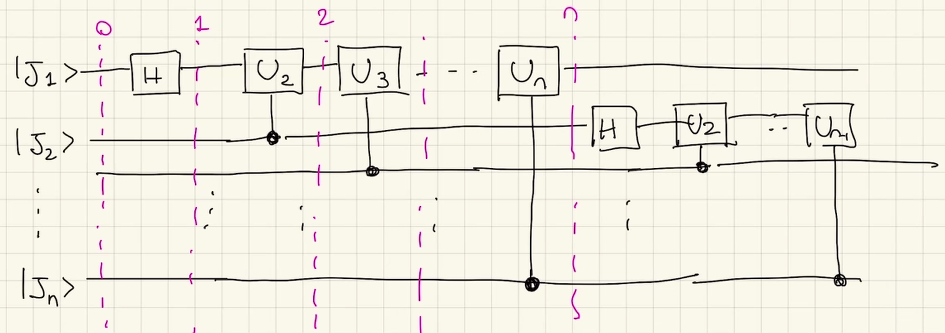
\includegraphics[scale=0.5]{25.png}
\end{center}
\begin{enumerate}
	\item $|j_1\ldots j_n\rangle$
	\item $H|j_1\rangle = \frac{1}{\sqrt{2}}\left(\ket{0} e^{\frac{2\pi i}{2}j_1}\ket{1}\right)\otimes |j_2\ldots j_n\rangle$
	\item Apply the gate only when $j_2$ is 1 (the black dot means that), but that's how $U$ works, it has a 0 on the $\ket{0}$\\
	$\frac{1}{\sqrt{2}}\left(\ket{0}+e^{\frac{2\pi i}{2}j_1}e^{\frac{2\pi i}{2^2}j_2}\ket{1}\right)\otimes|j_2\ldots j_n\rangle$
	\item $\frac{1}{\sqrt{2}}\left(\ket{0}+e^{\frac{2\pi i}{2}j_1}e^{\frac{2\pi i}{2^2}j_2}e^{\frac{2\pi i}{2^3}j_1}\ket{1}\right)\otimes|j_2\ldots j_n\rangle$
	\item[] \ldots
	\item[$n$.] $\frac{1}{\sqrt{2}}\left(\ket{0}+e^{2\pi i(\frac{j_1}{2}+\frac{j_2}{2^2}+\ldots+\frac{j_n}{2^n})}\ket{1}\right)\otimes|j_2\ldots j_n\rangle=$\\
	And given that 
	$j = \sum_{s=1}^nj_s 2^{n-s} = j_1 2^n+j_s^{n-1}+\ldots +j_n 2^0$ so we have
	$\frac{j_1}{2}+\frac{j_2}{2^2}+\ldots+\frac{j_n}{2^n} = \frac{1}{2^n}(j_1 2^n+j_s^{n-1}+\ldots +j_n 2^0)$ we have that\\
	$=\frac{1}{\sqrt{2}}\left(\ket{0} + e^{\frac{2\pi ij}{2^n}}\ket{1}\right)\otimes |j_2\ldots j_n\rangle$\\
	But we end up with the $n$th configuration on the first qubit!
\end{enumerate}
So we implements QFT in the reverse order, applying for example swap gates at the beginning or changing the configuration of the qubits at the end.
\paragraph{Review}
$$|\tilde{j}\rangle = QFT(j) = \frac{1}{\sqrt{N}}\sum_{k=0}^{N-1}e^{\frac{2\pi ijk}{N}}|k\rangle$$
$$|\tilde{j}\rangle = F_N|j\rangle$$
The $j$th column of $F_N$
$$F_N=\frac{1}{\sqrt{N}}\left[\begin{array}{c c c}
1&\ldots&1\\
\vdots& &\\
1
\end{array}\right]\hbox{ with the }(j,k)\hbox{ entry being }e^{\frac{2\pi ijk}{N}}$$
The circuit is
\begin{center}
	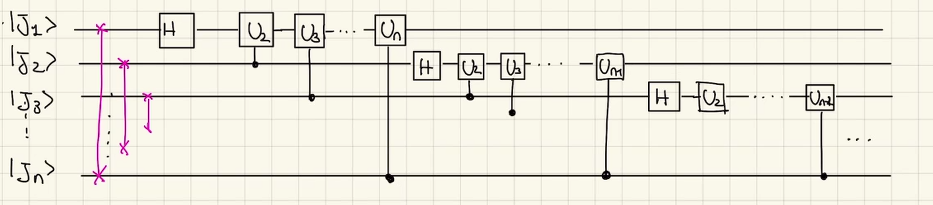
\includegraphics[scale=0.5]{26.png}
\end{center}
With the swap gates in purple.
\paragraph{Quantum Phase Estimation} Any unitary matrix is diagonalizable, has an orthonormal basis of eigenvectors and has a set of eigenvalues in the form $e^{i\theta_\psi}$ associated to an eigenstate $\ket{\psi}$
$$U\ket{\psi} = e^{i\theta_\psi}\ket{\psi}$$
The \textbf{QPE problem} is formulated as follows: given that we have the ability of preparing $\ket{\psi}$ and to use $U$, can we extract $\theta_\psi$ which is the angle of the rotation (the \textbf{phase})? Yes, also without QFT. Let's see the intuition on how we could do without QFT.
\begin{center}
	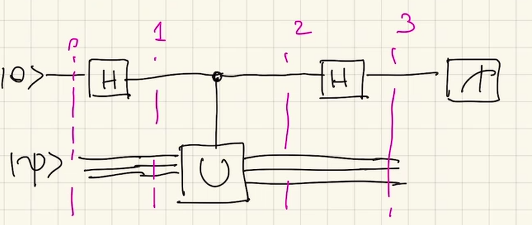
\includegraphics[scale=0.5]{27.png}
\end{center}
\begin{enumerate}
	\item My state is $\ket{0}\ket{\psi}$
	\item $\ket{\psi}$ doesn't change and we apply $H$ to $\ket{0}$ which becomes $\ket{+}$\\
	The state is $\frac{1}{\sqrt{2}}(\ket{0}+\ket{1})\ket{\psi} = \frac{1}{\sqrt{2}}\ket{0}\ket{\psi} + \frac{1}{\sqrt{2}}\ket{1}\ket{\psi}$
	\item $U$ applies only on the second qubit.\\
	The state is $\frac{1}{\sqrt{2}}\ket{0}\ket{\psi} + \frac{1}{\sqrt{2}}e^{i\theta_\psi}\ket{1}\ket{\psi}$
	\item $H\ket{0} = \ket{+}$ and $H\ket{1} = \ket{-}$, but $H$ applied only on the first qubit.\\
	The state is $\frac{1}{\sqrt{2}}(\frac{\ket{0}+\ket{1}}{\sqrt{2}})\ket{\psi} + \frac{1}{\sqrt{2}}e^{i\theta_\psi}(\frac{\ket{0}-\ket{1}}{\sqrt{2}})\ket{\psi} = \frac{1}{2}[(1+e^{i\theta_\psi})\ket{0} + (1-e^{i\theta_\psi})\ket{1}]\ket{\psi}$
\end{enumerate}
The probability of measuring $\ket{0}$ in the first qubit is the square of the amplitude. So we've encoded the information in the amplitudes, and they are different so I can distinguish them. The drawback is that we perform a complex circuit.\\\\
With QFE this is different. $\theta$ in general is $\in R$. The beginning of the QPE circuit is this:
\begin{center}
	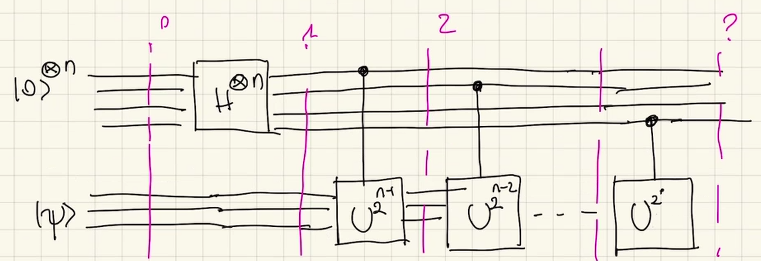
\includegraphics[scale=0.5]{28.png}
\end{center}
We apply a power of $U$: $U^{2^{n-1}}$ for $n$ bits, all the powers from $2^{n-1}$ to $2^0$.
\begin{enumerate}
	\item $\ket{0}^{\otimes n}\ket{\psi}$
	\item $\left(\frac{1}{\sqrt{2}}\right)^n (\ket{0}+\ket{1})^{\otimes n}\ket{\psi}$
	\item We have that $$U^k\ket{\psi} = \left(e^{i\theta_\psi}\right)^k\ket{\psi}$$
	The control bit is entangled, so by applying the $U$ gate the phase kicks back to the control bit.
	$$\left[\begin{array}{c c}
	I&\\
	&U
	\end{array}\right]\left(\left[\begin{array}{c}
	\alpha\\\beta
	\end{array}\right]\otimes\ket{\psi}\right)$$
	\item[Final.] $$\left(\frac{1}{\sqrt{2}}\right)^n (\ket{0}+e^{i\theta_\psi 2^{n-1}}\ket{1})\otimes(\ket{0}+e^{i\theta_\psi 2^{n-2}}\ket{1}|)\otimes\ldots\otimes(\ket{0}+e^{i\theta_\psi 2^{0}}\ket{1})\otimes\ket{\psi}$$
\end{enumerate}
Now we want to retrieve $\theta_\psi$. The QFT of $|j\rangle$ was $$|\tilde{j}\rangle = \frac{1}{\sqrt{N}}\left(\ket{0}+e^{\frac{2\pi ij}{2}}\ket{1}\right)\otimes\ldots\otimes\left(\ket{0}+e^{\frac{2\pi ij}{2^n}}\ket{1}\right)$$
These two configurations are very similar, they differ for the exponent. So it's the same of QPE except that $\theta_\psi$ is replace by $\frac{2\pi}{2^n}j$.\\
The final circuit is composed with the inverse of the QFT, where we need to run the circuit backwards, measuring $|2^n\theta_\psi\rangle$
\begin{center}
	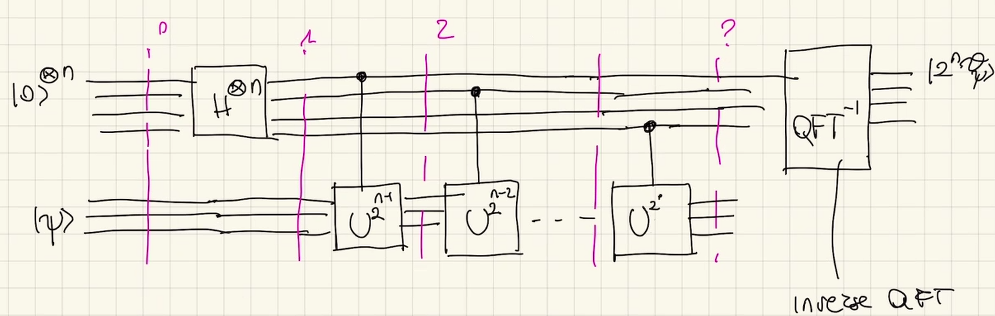
\includegraphics[scale=0.5]{29.png}
\end{center}
\subsection{Grover's Algorithm} 
Searching in an unstructured set of elements, from $O(N)$ to $O(\sqrt{N})$.\\We have a list of $N$ objects in a quantum memory and we want to retrieve a target element.\\
In the classical world, if the list is sorted we have $O(\log N)$ operations with binary search, otherwise in unsorted lists we may do on average $O(\frac{N}{2})$ accesses. In quantum we can do it in $O(\sqrt{N})$.
\paragraph{Example} Find $x,y,z,w\in N$ with $x,y,z,w\leq 10^6$ such that $x^4+y^4+z^4=w^4$. With a classical brute force approach we have a total number of queries of $\frac{10^{18}}{6}$ (removing permutations). With the quantum algorithm we can lower this number of queries to $\sqrt{N} = 10^9$.
\paragraph{Grover Iterations} If you have $M$ solutions (targets), you can lower the complexity to $O\left(\sqrt{\frac{N}{M}}\right)$\\
With $M=1$, assume the target solution is denoted by $\beta$, the oracle that recognizes the solution is $$\hbox{Oracle}(x) = \left\{\begin{array}{c l}
0&x=\beta\\1&x\neq\beta
\end{array}\right.$$
We need to represent in the quantum world this oracle: $U_\beta\ket{x}$. Our database is $\{\ket{0},\ldots,|N-\rangle\}$ with the usual convention that we are representing single qubits (so $\log N$ qubits from all zeros to all ones). This works by changing the phase
$$U_\beta\ket{x}=\left\{\begin{array}{l l}
\ket{x}&x\neq\beta\\-\ket{x}&x=\beta
\end{array}\right.$$
Identity if the state is $\neq\beta$
$$U_\beta = \left[\begin{array}{c c c c c}
1\\
&1\\
& &\ddots\\
& & &-1\\
& & & &\ddots\\
\end{array}\right]\hbox{ with }-1\hbox{ in position }(\beta,\beta)$$
$$U_\beta\ket{x}=(-1)^{\hbox{Oracle}(x)}\ket{x}$$
\paragraph{Construction of the Grover Oracle} Classical boolean functions can be converted to reversible quantum circuits.
$\ket{x}$ enters the circuit that output $\ket{x}$. The circuit is in xor with a $\ket{0}$ that emits $|f(x)\rangle$ such that if $f(x)=0$ nothing happens, so $\ket{0}\rightarrow\ket{0} = |f(x)\rangle$.\\
If $f(x) = 1$ then $\ket{0}\rightarrow\ket{1}=|f(x)\rangle$.
\begin{center}
	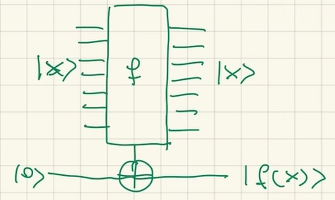
\includegraphics[scale=0.5]{30.png}
\end{center}
But we don't want to initialize it to $\ket{0}$ but to $\ket{-}$, such that the last register remains $\ket{-}$ and the Oracle outputs $(-1)^{f(x)}\ket{x}$
\begin{center}
	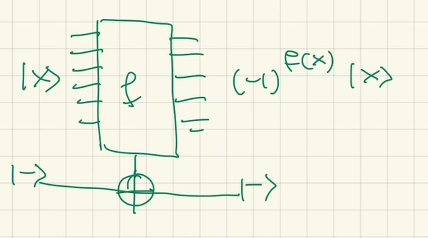
\includegraphics[scale=0.5]{31.png}
\end{center}
\paragraph{Grover Algorithm}
\begin{enumerate}
	\item Initialize the circuit to uniform superposition (usual Hadamard gates on each qubit), assuming $N=2^n$
	$$\ket{\psi}=\frac{1}{\sqrt{N}}\sum_{x=0}^{N-1}\ket{x}$$
	\item Perform $t$ times a \textbf{Grover Iteration}
	\item Measure in the computational basis
\end{enumerate}
The focus is $t$, which we are going to estimate, and proving that the Grover Iterations converge.
$$U_\beta\ket{\psi} = \frac{1}{\sqrt{N}}\sum_{x=0,x\neq\beta}^{N-1}\ket{x} - \frac{1}{\sqrt{N}}\ket{\beta}$$
Measuring will yield one of the $N$ configurations: we changed the phase but not the amplitude. So the Grover Iteration has the goal to amplify the amplitude of the target state in order to make it much bigger than the others.
\subparagraph{Diffuser} The goal is to amplify the amplitude of $\beta$.\\
Two important states:
\begin{list}{}{}
	\item $\ket{\psi}$ superposition of all the state
	\item $\ket{\beta}$ the target state
\end{list}
I consider $span\{\ket{\beta},\ket{\psi}\}$ which is a plane in $R^N$ (dimension 2). They are not orthogonal
$$\langle\beta\ket{\psi} = \frac{1}{\sqrt{N}}\neq 0$$
But for very large $N$ they are \textbf{almost orthogonal}.\\
We consider $\ket{\phi}\in span\{\ket{\beta},\ket{\psi}\}$ such that $\langle\phi\ket{\beta}=0$: we can take $\ket{\psi}$ and remove the components in directions of $\ket{\beta}$
$$\ket{\phi}=\sqrt{\frac{N}{N-1}}\left(\frac{1}{\sqrt{N}}\sum_{x=0}^N\ket{x}\right)-\frac{1}{\sqrt{N}}\ket{\beta} = \frac{1}{\sqrt{N-1}}\sum_{x\neq\beta}\ket{x}$$
We can also rewrite $\ket{\psi}$
$$\ket{\psi} = \sin\left(\frac{\theta}{2}\right)\ket{\beta} + \cos\left(\frac{\theta}{2}\right)\ket{\phi} = \frac{1}{\sqrt{N}}\ket{\beta} + \sqrt{\frac{N-1}{N}}\ket{\phi}$$
Because $\sin\frac{\theta}{2} = \frac{1}{\sqrt{N}}\Leftrightarrow\frac{\theta}{2}=\arcsin\frac{1}{\sqrt{N}}$. So the angle between $\ket{\psi}$ and $\ket{\phi}$ is $\frac{\theta}{2}$
\begin{center}
	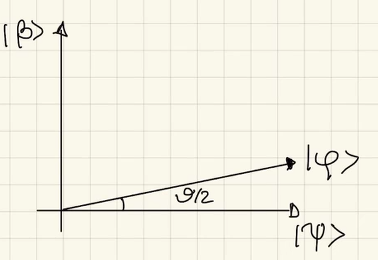
\includegraphics[scale=0.5]{32.png}\\
	$\psi$ and $\phi$ are inverted
\end{center}
So we start and apply $U_\beta$ to our starting state $\ket{\psi}$
$$U_\beta\ket{\psi} = \cos\frac{\theta}{2}\ket{\phi}-\sin\frac{\theta}{2}\ket{\beta}$$
So it reflects along $\ket{\phi}$: $U_\beta$ is a reflection along the space orthogonal to $\ket{\beta}$.
\begin{center}
	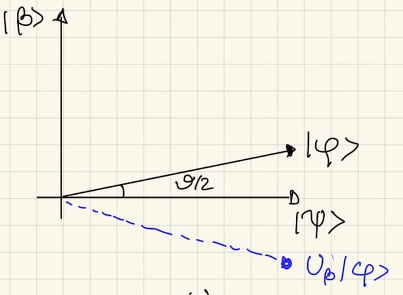
\includegraphics[scale=0.5]{33.png}\\
	$\psi$ and $\phi$ are inverted
\end{center}
Starting with all equal amplitudes of $\frac{1}{\sqrt{N}}$, the amplitude of $\ket{\beta}$ is inverted!
\begin{center}
	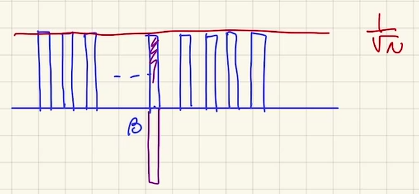
\includegraphics[scale=0.5]{34.png}
\end{center}
Then the diffuser step $U_\psi$: reflection around $\ket{\psi}$
$$U_\psi = 2\ket{\psi}\langle\psi|-I$$
We obtain $U_\psi U_\beta\ket{\psi}$ which reflects $U_\beta\ket{\psi}
$ around $\ket{\psi}$ with an angle of $\theta$ with $\ket{\psi}$
\begin{center}
	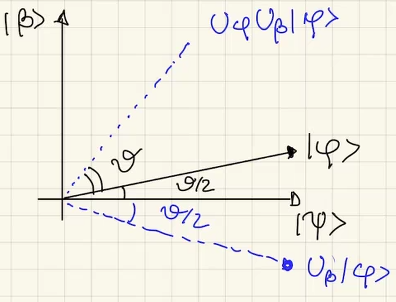
\includegraphics[scale=0.5]{35.png}\\
	$\psi$ and $\phi$ are inverted
\end{center}
This reflection is often referred to as inversion around the average. The amplitudes of the configurations $\neq\ket{\beta}$ is lowered to $\frac{N-2}{N\sqrt{N}}$ while the amplitude of $\ket{\beta}$ is amplified.\\
These reflections are the iterations: start with $\ket{\psi}$, reflect along the $\ket{\phi}$ orthogonal to the target $\ket{\beta}$ and then reflect along $\ket{\psi}$ obtaining $\ket{z}$. Then repeat: reflect $\ket{z}$ along $\ket{\phi}$, reflect along $\ket{\psi}$\ldots\\At the generic step\begin{list}{}{}
	\item $G=U_\psi U_\beta$
	\item $|\psi^{(k)}\rangle = G^k\ket{\psi} = G|\psi^{(k-1)}\rangle$
\end{list}
Let's denote
$$\ket{z} = U_\beta|\psi^{(k)}\rangle = \sum_{x=0}^{N-1}\alpha_x\ket{x}$$
$$|\psi^{(k+1)}\rangle=U_\psi\ket{z} = (2\ket{\psi}\langle\psi| - I)\left(\sum_{x=0}^{N-1}\alpha_x\ket{x}\right) = 1\sum_{x=0}^{N-1}\alpha_x\langle\psi\ket{x}\ket{\psi}-\sum_{x=0}^{N-1}\alpha_x\ket{x} = $$
$\langle\psi\ket{x} = \frac{1}{\sqrt{N}}$ and $\ket{\psi}$ doesn't depend on $\ket{x}$
$$2\sum_{x=0}^{N-1}\frac{1}{\sqrt{N}}\alpha_x = \frac{2N}{\sqrt{N}}\frac{1}{N}\sum_{x=0}^{N-1}\alpha_x$$
The $M = \frac{1}{N}\sum_{x=0}^{N-1}\alpha_x$ is the average of $z$ so we can rewrite as
$$|\psi^{(k+1)}\rangle=\sum_{x=0}^{N-1}(-\alpha_x + 2M)\ket{x}$$
The first step
$$|\psi^{(1)}\rangle = \left(2M-\frac{1}{\sqrt{N}}\right)\sum_{x\neq\beta}\ket{x}+\left(2M+\frac{1}{\sqrt{N}}\right)\ket{\beta}$$
Can see that the amplitude of $\ket{\beta}$ has increased and the others have decreased by a factor proportional to the mean.
\paragraph{Number of Iterations}
$G = U_\psi U_\beta$ is a rotation: \textbf{the composition of two reflectors is a rotation} of an angle $\theta$ where $\sin\frac{\theta}{2}=\frac{1}{\sqrt{N}}\Leftrightarrow\theta = 2\arcsin\frac{1}{\sqrt{N}}$.\\
$G^k$ has rotated of $\theta^k = (2k+1)\frac{\theta}{2}$ and we want to stop when $(2k+1)\frac{\theta}{2}=\frac{\pi}{2}$, near $\ket{\beta}$ (at 90 degrees).
$$k\theta + \frac{\theta}{2} = \frac{\pi}{2}$$
$$k = \left(\frac{\pi}{2}-\frac{\theta}{2}\right)\frac{1}{\theta}$$
But $\frac{\pi}{2}$ is irrational so we want an approximation
$(2k+1)\frac{\theta}{2}\simeq\frac{\pi}{2}$
$$k=\lfloor\frac{\pi}{2\theta}-\frac{1}{2}\rfloor$$
For a sufficiently large $N$ we can approximate $\arcsin\left(\frac{\theta}{2}\right) = \frac{\theta}{2} = \frac{1}{\sqrt{N}}$ (from the Taylor expansion of $\arcsin$) getting
$$k\simeq\left(\frac{\pi}{2}-\frac{1}{\sqrt{N}}\right)\frac{\sqrt{N}}{2} = \frac{\pi}{4}\sqrt{N}-\frac{1}{2}$$
So the number of iterations $$t\simeq\frac{\pi}{4}\sqrt{N}$$
\begin{center}
	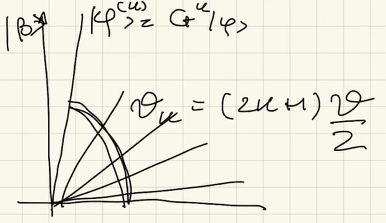
\includegraphics[scale=0.5]{36.png}
\end{center}
The remaining angle is $\frac{\pi}{2}-(2k+1)\frac{\theta}{2}$
\subparagraph{Theorem} If we perform $k=\lfloor\frac{\pi}{2\theta}-\frac{1}{2}\rfloor\simeq\frac{\pi}{4}\sqrt{N}$ Grover Iterations, the probability of measuring the target state $\ket{\beta}$ is $$P(\hbox{Measuring }\ket{\beta}) = 1-\frac{1}{N}$$
Projecting along $\ket{\beta}$ at time $k$
$$P(\hbox{Measuring }\ket{\beta}) = |\langle\beta|\:G^k\ket{\psi}|^2 = \cos^2\left(\frac{\pi}{2}-(2k+1)\frac{\theta}{2}\right) = 1-\sin^2\left(\frac{\theta}{2}\right) = 1-\frac{1}{N}$$
\paragraph{Circuit for the Grover Iteration $G$}
We have $H^{\otimes n}\ket{\psi} = \ket{0}^{\otimes n}$ so $\ket{\psi} = H^{\otimes n}\ket{0}$, also $I = H^{\otimes n}H^{\otimes n}$
$$U_\psi=2\ket{\psi}\langle\psi|-I = H^{\otimes n}(2\ket{0}\langle0|-I)H^{\otimes n}$$
$$2\left[\begin{array}{c c c c c}
1\\\\&&0\\&&&\\
\end{array}\right]-\left[\begin{array}{c c c}
1\\&\ddots\\&&1
\end{array}\right] = \left[\begin{array}{c c c c}
1\\&-1\\&&\ddots\\&&&-1
\end{array}\right]$$
\subsection{Shor's Algorithm} $N$ composite number: Shor's algorithm can find a factor of $N$ in $O(n^2\cdot\log n\cdot\log\log n)$ steps, with $n=\lceil\log N\rceil$. Can find factors in NP.\\
The most efficient classical factoring algorithm (general number field sieve) works in subexponential $O(e^{1.9}n^{1/3(\log n)^{2/3}})$\\
The decision version of the problem is not NP-complete. All current public key cryptography (RSA, DH, ECC) would be broken if Shor's algorithm could be physically realized.
\paragraph{Complexity Classes}
\begin{list}{}{}
	\item \textbf{BQP} (Bounded-error Quantum Polynomial Time): class of decision problems that can be solved in polynomial time on a quantum computer, with bounded error probability (at most $1/3$ as arbitrary choice, can be $1/2$)\\
	The decision version of factoring is in BQP
	\item \textbf{BPP} (Bounded-error Polynomial Time): class of decision problems that can be solved in polynomial time using randomized algorithms, if a bounded probability of error is allowed in the solution.\\
	The decision version of factorization is not known to be in BPP.
\end{list}
If indeed factorization $\not\in$ BPP, then quantum computer would be the first counterexample to the "strong" Church-Turing Thesis, which states that all reasonable models of computation are polynomially equivalent.\\\\
Application of QPE: quantum order-finding. Factorization is solved via a reduction to order-finding.
\paragraph{Order-Finding Problem} We are given coprime integers $a, N$, meaning GCD$(a,N)=1$. The \textbf{order}/period of $a$ is the smallest positive integer $r$ such that $$a^r\hbox{ mod }N = 1$$
The problem is finding $r$ given $a$ and $N$ with GCD$(a,N)=1$.\\
Also called period because $f(x) = a^x\hbox{ mod }N$ is periodic with period $r$. Indeed $\forall\:s\:\:f(s+r)=a^{s+r}\hbox{ mod }N = a^s\hbox{ mod }N = f(s)$
\paragraph{Shor's Algorithm} The idea is to use QPE: given $U\ket{\psi}=e^{2\pi i\theta}\ket{\psi}$ with $\ket{\psi}$ eigenvector and $e^{2\pi i\theta}$ corresponding eigenvalues.
\begin{center}
	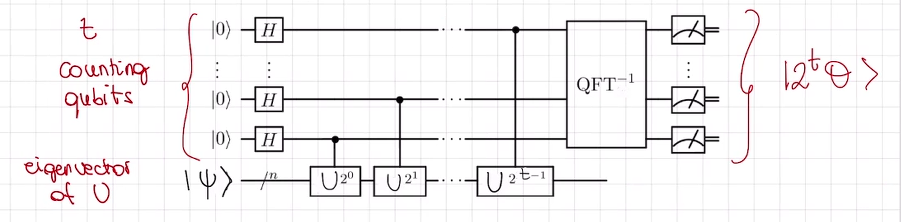
\includegraphics[scale=0.5]{37.png}
\end{center}
The accuracy and the probability of success of QPE depends on the number of counting qubits $t$. Need to define a unitary operator that computes $$f(x) = a^x\hbox{ mod }N$$ and whose eigenvalues contain the order $r$, so that we can apply QPE to estimate the eigenvalues and recover $r$.
\paragraph{Construction of $U_a$} Given $N, n=\lceil\log_2N\rceil, a$
$$U_a|y\rangle=\left\{\begin{array}{ll}
|a\cdot y\hbox{ mod }N\rangle&0\leq y<N\\
|y\rangle&N\leq y< 2^n
\end{array}\right.$$
Example with $N=5, a=3, n=3$$$U_a|y\rangle=\left\{\begin{array}{ll}
|3\cdot y\hbox{ mod }5\rangle&0\leq y<6\\
|y\rangle&6\leq y< 8
\end{array}\right.$$
Show that $U_a$ is unitary and that it contains the eigenvalue $r$.
\subparagraph{$U_a$ is unitary} It can be described by a block diagonal matrix.\begin{center}
	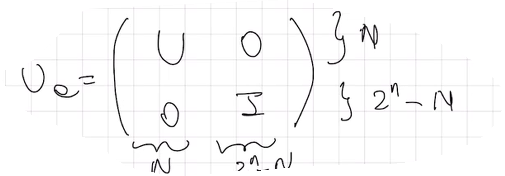
\includegraphics[scale=0.5]{38.png}
\end{center}
So to prove that $U_a$ is unitary it's enough to prove that $U$ is unitary, so that $U^+U = I$. Given $0\leq y',y<N$, we need to prove that
$$\langle y'|U^+U|y\rangle = \delta_{yy'} = \left\{\begin{array}{l l}
0&y\neq y'\\
1&y=y
\end{array}\right.$$
So we have $$\langle y'|U^+U|y\rangle = <ay'\hbox{ mod }N|ay\hbox{ mod }N\rangle$$
This can happen $\Leftrightarrow$
$$ay'\equiv ay\hbox{ mod }N$$
Remember that $a$ is coprime with $N$, so we have that $\exists\:a^{-1}$
$$a^{-1}ay'\equiv a^{-1}ay\hbox{ mod }N$$
$$y'\equiv y\hbox{ mod }N$$
And $y,y'<N$ so we have an equivalence
$$y' = y$$
So the operator is unitary.
\subparagraph{Eigenvalues of $U_a$} We have $$U_a^r|y\rangle = U_a^{r-1}|ay\hbox{ mod }N\rangle = \ldots = |a^ry\hbox{ mod }N\rangle = |y\rangle$$
Because $r$ is the order. So we have $$U_a^r|y\rangle = \left\{\begin{array}{ll}
|y\rangle&0\leq y<N\\
|y\rangle&N\leq y<2^n
\end{array}\right.$$
So $U_a^r = I$ is the identity. This means that the eigenvalues of $U_a$ are the $r$-roots of the unity.
$$\lambda_s = e^{\frac{2\pi i}{r}s} = \omega^s$$ with $0\leq s<r$ and $e^{\frac{2\pi i}{r}} = \omega$\\
The phase is $\frac{s}{r}$, and it contains $r$.
\subparagraph{Eigenvectors of $U_a$} $\forall\:0\leq s< r$ $$|u_s\rangle = \frac{1}{\sqrt{r}}\sum_{k=0}^{r-1}\omega^{-sk}|a^k\hbox{ mod }N\rangle$$
is the eigenvector with eigenvalues $\omega^s == e^{\frac{2\pi i}{r}s}$\\
$$U_a|u_s\rangle = \frac{1}{\sqrt{r}}\sum_{k=0}^{r-1}\omega^{-sk}|a^{k+1}\hbox{ mod }N\rangle =$$ $$= \frac{1}{\sqrt{r}}\sum_{k=1}^{r}\omega^{-s(k-1)}|a^k\hbox{ mod }N\rangle =$$ $$=\frac{1}{\sqrt{r}}\sum_{k=1}^{r-1}\omega^s\omega^{-sk)}|a^k\hbox{ mod }N\rangle + \frac{1}{\sqrt{r}}\omega^s\omega^{-sr}|a^r\hbox{ mod }N\rangle= $$ We have that, in the term corresponding to $k=r$, $\omega^{-sr}=1$ and $a^r=1$ by definition of order $$=\frac{1}{\sqrt{r}}\omega^s\sum_{k=1}^{r-1} \omega^{-sk}|a^k\hbox{ mod }N\rangle + \frac{1}{\sqrt{r}}\omega^s\omega^{-s0}|a^0\hbox{ mod }N\rangle  =$$ Observe that the term corresponding to $k=r$ is equal to the term corresponding to $k=0$.
$$=\frac{1}{\sqrt{r}}\omega^s\sum_{k=0}^{r-1}\omega^{-sk}|a^k\hbox{ mod }N\rangle = \omega^s|u_s\rangle$$
$$U_a|u_s\rangle = \omega^s|u_s\rangle$$
$$\omega^s=e^{\frac{2\pi i}{r}s}$$
To run QPE we need to prepare the state $|u_s\rangle$, but to prepare it we need $r$ which we do not have.\\
Instead of preparing $|u_s\rangle$ we prepare a superposition of the eigenvectors.
$$\frac{1}{\sqrt{r}}\sum_{s=0}^{r-1}|u_s\rangle =\frac{1}{\sqrt{r}}\sum_{s=0}^{r-1}\frac{1}{\sqrt{r}}\sum_{k=0}^{r-1}\omega^{-sk}|a^k\hbox{ mod }N\rangle =$$
$$ = \frac{1}{r}\sum_{s=0}^{r-1}\left( \omega^{-0s}|a^0\hbox{ mod }N\rangle+\sum_{k=1}^{r-1}\omega^{-sk}|a^k\hbox{ mod }B\rangle \right) =$$
$$= \frac{1}{r}\sum_{s=0}^{r-1}\ket{1}+\frac{1}{r}\sum_{k=1}^{r-1}\left(\sum_{s=0}^{r-1}\omega^{-sk}\right)|a^k\hbox{ mod} N\rangle =$$
$$=\ket{1} + \frac{1}{r}\sum_{k=1}^{r-1}\left(\frac{1-(\omega^{-sk})^r}{1-\omega^{-sk}}\right)|a^k\hbox{ mod }N\rangle =$$
And $\omega = e^{\frac{2\pi i}{r}}$ so the sum in parenthesis is $0$, so the superposition of all the states is just 
$$=\ket{1} = |0\ldots01\rangle$$
with $n-1$ zeros and a $1$, so $n=\lceil\log N\rceil$ bits.
\paragraph{Circuit} QPE circuit adapted\begin{center}
	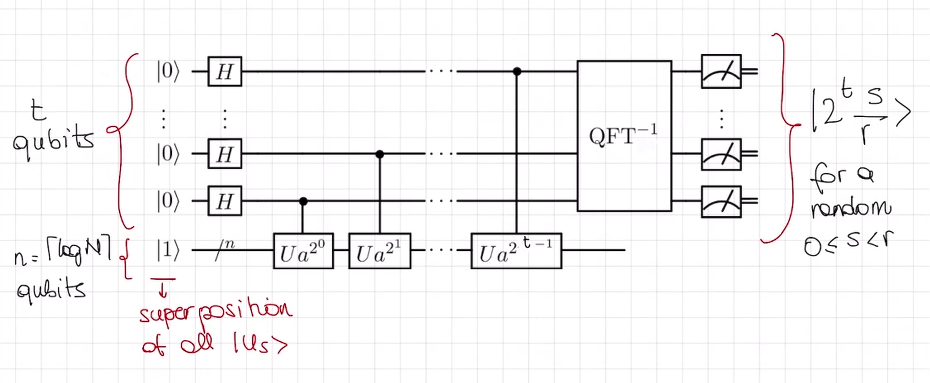
\includegraphics[scale=0.5]{39.png}
\end{center}
$$ t= 2n+1+\lceil\log\left(2+\frac{1}{2\epsilon}\right)\rceil$$
With $t$ qubits we will obtain an estimate of $\frac{s}{r}$ accurate to $2n+1$ bits with probability of at least $1-\epsilon$. We need that accuracy to be able to recover $r$ from the phase $\frac{s}{r}$ (with a classical algorithm).\\
The circuit consists of 4 steps
\begin{enumerate}
	\item Apply $t$ Hadamard gates to put the first counting qubits register in equal superposition.
	$$\ket{0}^{\otimes n}\ket{1}\mapsto \frac{1}{\sqrt{2^t}}\sum_{j=0}^{t-1}|j\rangle\ket{1}$$
	\item Apply the sequence of controlled $U_a^{2^j}$ gates with control on the $j$th qubit.
	$$\frac{1}{\sqrt{r\cdot2^t}}\sum_{s=0}^{r-1}\sum_{j=0}^{2^t-1}\omega^{sj}|j\rangle|u_s\rangle$$
	\item Apply the inverse Quantum Fourier Transform on the first register and we get a superposition of eigenvectors $|u_r\rangle$ entangled with estimates of their corresponding eigenvalues
	$$\frac{1}{\sqrt{r}}\sum_{s=0}^{r-1}|2^t\frac{s}{r}\rangle|u_s\rangle $$
	So a superposition of estimates instead of a single estimate like in QPE
	\item Measure the first register, and since there is a superposition we have each estimate with equal probability. The uniform superposition collapses to one of the $r$ eigenvectors $|u_s\rangle$ and QPE returns an estimate of the phase $\frac{s}{r}$ for a random (unknown) $s$ with $0\leq s< r$
\end{enumerate}
\paragraph{Implementing $U_a$ Efficiently} Using fast exponentiation: square and multiply (quadrature successive).\\
The idea is that $$U_a^{2^j}|y\rangle = |a^{2^j}y\hbox{ mod }N\rangle =$$
But we take the modulo immediately
$$= |(a^{2^j}\hbox{ mod }N)y\hbox{ mod }N\rangle$$
So we precompute all values $$a\hbox{ mod }N,a^2\hbox{ mod }N,a^4\hbox{ mod }N,\ldots,a^{2^j}\hbox{ mod }N,\ldots,a^{2^{t-1}}\hbox{ mod }N$$
These are all $n$ bit numbers, and we can compute all of them with $t-1$ operations, $O(n^2)$ or $O(n\log n\log\log n)$ with fast multiplication. $t$ is $O(n)$ therefore the cost is $O(n^2\log n\log\log n)$ with fast multiplication.
$$U_a^{2^j}|y\rangle = |(a^{2^j}\hbox{ mod }N)y\hbox{ mod }N\rangle$$
\paragraph{Recovering $r$ from the Phase $\frac{r}{s}$} This is classical computation, doesn't require quantum computation and is performed on a classical computer applying the \textbf{Continued Fractions Algorithm} CFA.\begin{list}{}{}
	\item On the first register we measure an integer $x=2^t\frac{s}{r}$ for unknown $r$ and $s$.\\
	So $\frac{x}{2^t}=\phi \simeq \frac{s}{r}$ is an estimate, we only know $2n+1$ bits of $\phi$.
	\item \textbf{Easy case}\\
	Suppose that $r$ divides $2^t$, then we know exactly $\phi$ because $\frac{x}{2^t}=\frac{s}{r}$\\
	The fraction is known because we know $x$ and $t$, and to get $r$ we reduce the fraction $\frac{x}{2^t}$ to the lowest terms (to an irreducible fraction). Then we test the denominator $r'$ if it's $r$: we compute $a^{r'}\hbox{ mod }N$ and if its $1$ we're done.\\
	This works if $r,s$ are coprime.
	\item \textbf{General case}\\
	We don't know $\phi$ exactly but just $2n+1$ bits of $\phi$. We apply CFA to compute the nearest fraction to $\phi$ with denominator $\leq N$. We take this denominator as tentative order, as $r'$.\\
	This produces the fraction $\frac{s'}{r'}$ with $s',r'$ without common factors, and we check whether $a^{r'}\hbox{ mod }N =1$. If so, we're done, else we run again. Even in this case, the procedure requires $r,s$ coprime.
\end{list}
\subparagraph{Quantum Order Finding}
\begin{enumerate}
	\item Initial state is $\ket{0}\ket{1}$ ($t$ and $n$ qubits)
	\item Create a superposition on the first register $$\frac{1}{\sqrt{2^t}}\sum_{j=0}^{2^t-1}|j\rangle\ket{1}$$
	\item Apply the sequence of controlled $U_a^{2^j}$ gates
	 $$\frac{1}{\sqrt{r2^t}}\sum_{s=0}^{r-1}\sum_{j=0}^{2^t-1}e^{\frac{2\pi isj}{r}}|j\rangle|u_s\rangle$$
	 \item Apply inverse Fourier transform to the first register
	 $$\frac{1}{\sqrt{r}}\sum_{s=0}^{r-1}|2^t\frac{s}{r}\rangle|u_s\rangle$$
	 \item Measure the first register, estimating $\psi$ of $\frac{s}{r}$
	 \item Apply CFA obtaining $r$
\end{enumerate}
The overall cost for order-finding with fast multiplication is $O(n^2\log n\log\log n)$, while the best classical algorithm is $O(e^{\sqrt{n\log n}})$, but of course the quantum algorithm can fail because QPE can produce a bad estimate for $\frac{s}{r}$ with probability at most $\epsilon$ thanks to our choice of $t$.\\
If $r,s$ have a common factor, the number $r$ returned but the CFA is a factor of $r$, not $r$ itself. So $r,s$ should be co-prime.
\paragraph{Factorization $\leq$ Order-Finding} Reduction from factoring to order-finding.\\
$N>1$ composite, odd and not a prime nor a prime power (we can already test these cases and exclude them in the beginning). So $N$ is a product of at least two primes.\\
We take $a< N$ and coprime with $N$ (GCD$(a,N)=1$). If it's not coprime, we've found a factor of $N$. Suppose that is coprime. We compute the order $r=$ Order($a$). So we know that $a^r$ mod $N=1$, which can be written as $$(a^r-1)\hbox{ mod }N = 0$$
Suppose that $r$ is even, we can write
$$(a^{\frac{r}{2}}-1)(a^{\frac{r}{2}}+1)\hbox{ mod }N = 0$$
$1<a<N$ so the possible cases are:\begin{list}{}{}
	\item The first factor $a^{\frac{r}{2}}-1\hbox{ mod }N = 0$
	But this means $$a^{\frac{r}{2}}\hbox{ mod }N = 1$$ which is impossible per definition of order.
	\item We could have the second factor $a^{\frac{r}{2}}+1\hbox{ mod }N = 0$ means that 
	$$a^{\frac{r}{2}}\hbox{ mod }N = -1$$
	This can happen, the reduction fails and we need to start over with a different $a$
	\item Both terms are $\neq0\hbox{ mod }N$, this means that $N$ divides $(a^{\frac{r}{2}}-1)(a^{\frac{r}{2}}+1)$ and any factor of $N$ is a factor of $(a^{\frac{r}{2}}-1)$ or $(a^{\frac{r}{2}}+1)$ or both. This factor cannot be $N$ (excluded before, non zero modulo $N$).\\
	Using Euclid's algorithm we compute GCD($a^{\frac{r}{2}}-1,N$) and GCD($a^{\frac{r}{2}}+1,N$) and find a factor of $N$.
\end{list}
\paragraph{Shor's Algorithm} 
Input: a positive integer $N$ with $n=\lceil\log_2 N\rceil$ bits.\\
Output: a factor $p$ of $N$
\begin{enumerate}
	\item If $N$ is even, output 2 and stop
	\item Use a polynomial time algorithm to determine if $_N$ is a prime or a power of a prime. If this is the case, declare it and stop.
	\item Randomly choose an integer $a$ such that $1<a<N$ and run Euclid's algorithm to determine $GCD(a,N)$. If it's $>1$, return it and stop.
	\item If $a$ and $N$ are coprime, use a Quantum Circuit to find the order $r$ of $a$ mod $N$
	\item If $r$ is even and $a^{r/2}$ mod $N\neq -1$ compute GCD($a^{\frac{r}{2}}-1,N$) and GCD($a^{\frac{r}{2}}+1,N$) and return at least one non trivial factor of $N$.\\
	Otherwise
\end{enumerate}
\paragraph{Observations} The algorithm returns with high probability a non trivial factor of any composite $N$.\\
All steps can be performed efficiently on a classical computer, except (as far as we know) the order-finding step (step 4). By repeating the procedure, we may find a complete prime factorization of $N$.
\paragraph{Complexity} Polynomial in $n=\lceil\log_2 N\rceil$. It take $O(n^2\log n\log\log n)$ quantum gates using fast multiplication and the square-and-multiply algorithm.
\paragraph{Success Probability} A single run only returns a factor of $N$ with a certain probability.\begin{list}{}{}
	\item The order-finding step could return an odd $r$
	\item The order-finding step could return $r\:|\:a^{r/2}\hbox{ mod }N \equiv -1$
	\item The reduction to the order-finding problem doesn't work if $r\equiv 1\hbox{ mod }2$ or $a^{r/2}\hbox{ mod }N \equiv -1$
\end{list}
\subparagraph{Theorem} Let $N = \prod_{j=1}^kp_j^{n_j}$ be the factorization of $N$, with $p_i\neq p_j$ for $i\neq j$. If $a$ is a random element in $Z_N^*$ (i.e. $0<a<N$ and coprime with $N$), and $r = order(a)$ then
$$P\left(r\equiv 0\hbox{ mod }2\wedge a^{r/2}\not\equiv -1\hbox{ mod }N\right)\geq 1-\frac{1}{2^k}$$
The algorithm only needs to be repeated a constant number of times to successfully factor $N$ with a high probability of success. The expected number of iterations needed to find a factor doesn't grow with $N$. Shor's algorithm can factor in a number of operations polynomial in the dimension of $N$.\\
\textbf{Exponential speed-up} compared to the best classical algorithm.
\section{Quantum AI} Typically, classical AI algorithms require high computational resources. Can Quantum Computing "boost" AI algorithms? Yes and no, at the same time, in a typical QC fashion.\\
We will see three building blocks for QAI:
\begin{list}{}{}
	\item Recall the idea of classical KNN
	\item Define its quantum counterpart, QKNN
	\item Show the circuit by hand (and by code in Qiskit)
\end{list}
\paragraph{KNN} Given a dataset $D = \langle x,y\rangle$ of instances $x$ labeled by $y$, and an unseen instance $t$, we want to find the label $$y_t = \arg\max_{v\in V} \sum_{(x_i,y_i) \in N_t} I(v_i, y_i)$$
with $v\in V$ being the class labels and $(x_i,y_i)$ the instances in the neighborhood $N_t$ of $t$.\\
Means assigning to $t$ the label among $|V|$ labels according to a majority voting over the neighborhood of $t$ ($N_t$).\\
So we compute the distances from $t$ to each element in its neighborhood. QKNN does this in just one shot. \textbf{All the distances are computed simultaneously}, this feature is called \textbf{quantum parallelism}.
\paragraph{Building Blocks Needed} Few questions need to be addressed:
\begin{enumerate}
	\item How to encode classical data in a quantum circuit?
	\item How can we compute the distances in the quantum circuit world?
	\item Where do we store the data?
\end{enumerate}
\subsection{Data Encoding}
\paragraph{1st Building Block} Given a quantum state $\ket{\psi}=\alpha\ket{0} + \beta\ket{1}$, where can we encode information?
\paragraph{Basis encoding} I.e. $5\mapsto bin(5)\mapsto 101\mapsto |101\rangle$\\
	To encode:
	\begin{center}
	\begin{quantikz}
		\lstick{$\ket{0}$} & \gate{X} & \qw & \rstick{$\ket{1}$}\\
		\lstick{$\ket{0}$} & \qw & \qw & \rstick{$\ket{0}$}\\
		\lstick{$\ket{0}$} & \gate{X} & \qw & \rstick{$\ket{1}$}\\
	\end{quantikz}
	\end{center}
\paragraph{Amplitude encoding} Encode information in $\alpha$ and $\beta$.\\
For simplicity, we assume that our classical data are all already normalized. Why?
$$|\alpha|^2+|\beta|^2 = 1$$
$$|\alpha|^2 = \left(\sqrt{\alpha^T\alpha}\right)^2$$
Qubits can be mapped onto a sphere, the Bloch sphere.
\begin{center}
	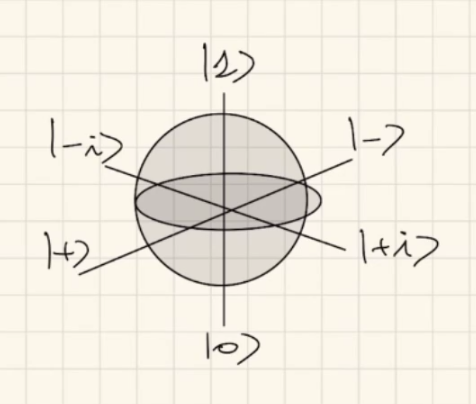
\includegraphics[scale=0.5]{40.png}
\end{center}
$$\ket{\psi} = \cos\theta\ket{0} + \sin\theta\ket{1}$$
$$\cos\theta = \alpha$$
$$\sin\theta = \beta$$
We want to remove the $\ket{-i}$ and $\ket{+i}$, so that the Block sphere becomes a circumference.
\begin{center}
	\begin{tikzpicture}[scale=1.5]
		
		\draw[-]  (-1.25cm,0cm) node[left] {$\ket{-}$} -- (1.25cm,0cm) node[right] {$\ket{+}$};
		\draw[-]  (0cm,-1.25cm) node[below] {$\ket{0}$} -- (0cm,1.25cm) node[above] {$\ket{1}$};
		\draw   (0cm,0cm) circle(1cm);
	\end{tikzpicture}
\end{center}
\subparagraph{Example} $x_0 = 1$ our datapoint that we want to encode in the qubit. We need the $\arcsin$ function, we'll see later why.
$\arcsin(1)$ is the angle such that its $\sin$ is 1, $\arcsin(1) = \frac{\pi}{2}$
$$\ket{\psi} = \alpha\ket{0} + \beta\ket{1} = \cos\theta\ket{0} + \sin\theta\ket{1}$$
We apply $R_y$ gate, rotation, on $\ket{\psi}$ to encode $x_0$.
$$R_y(\theta) = \left(\begin{array}{c c}
\cos\frac{\theta}{2} & -\sin\frac{\theta}{2}\\
\sin\frac{\theta}{2} & \cos\frac{\theta}{2}
\end{array}\right)$$
\begin{center}
	\begin{tikzpicture}[scale=1.5]
		
		\draw[-]  (-1.25cm,0cm) node[left] {$\ket{-}$} -- (1.25cm,0cm) node[right] {$\ket{+}$};
		\draw[-]  (0cm,-1.25cm) node[below] {$\ket{0}$} -- (0cm,1.25cm) node[above] {$\ket{1}$};
		\draw   (0cm,0cm) circle(1cm);
		\draw (0cm,0cm) -- (-0.72cm, 0.72cm) node[above] {$x_j$};
	\end{tikzpicture}
\end{center}
If we want to move $x_s = \ket{0}$ to $\ket{+} = \frac{1}{\sqrt{2}}(\ket{0}+\ket{1})$ we need to apply a 90 degree rotation. If we want to encode $\frac{1}{2}$, we need $\arcsin(\frac{1}{2}) = \frac{\pi}{6}$
\subsection{Distances} We'll focus on Euclidean distance.
$$d(\psi, \delta) = \sqrt{(\psi_x - \delta_x)^2-(\psi_y-\delta_y)^2} = \|\psi-\delta\|$$
\subparagraph{Quantum Euclidean Distance} 
	\begin{center}
	\begin{quantikz}
		\lstick{$\ket{0}_e$} & \gate{H} & \ctrl{1} & \gate{X} & \ctrl{1} & \gate{H} & \meter{$0$}\\
		\lstick{$\ket{0}$} & \qw & \gate{R_y(\theta_\psi)} & \qw & \gate{R_y(\theta_\delta)} & \qw & \qw \rstick{$\ket{\hbox{res}}$}\\
	\end{quantikz}
	\end{center}
The gate $R_y(\theta_\psi$ corresponds to amplitude encoding the value $\psi$, and the \begin{quantikz} \meter{$0$}\end{quantikz} gate means we measure only when the qubit $e$ is $0$. Why does it work?
\begin{enumerate}
	\item We start from $\ket{0_e0}$ and put into superposition the first qubit
	$$|0_e0\rangle \Rightarrow \frac{1}{\sqrt{2}}(\ket{0}+\ket{1})\ket{0} = \frac{1}{\sqrt{2}}(\ket{00}+\ket{10})$$
	\item Encode $\psi$, the first datapoint, by means of a C$_{e=1}$R$_y$($\theta_\psi$) (a controlled rotation on axis $y$ on $\theta_\psi$). Controlled on qubit $e$, so the rotation occurs when $e$ it's equal to $1$.
	$$\Rightarrow \frac{1}{\sqrt{2}}(\ket{00}+\ket{1\psi})$$
	\item Encode $\delta$, the second datapoint, by means of a C$_{e=1}$R$_y$($\theta_\delta$). Triggers when the first qubit is $1$, so we need the $X$ rotation.\\
	So $X$ gate on $e$
	$$\Rightarrow \frac{1}{\sqrt{2}}(\ket{10}+\ket{0\psi})$$
	and then the controlled rotation
	$$\Rightarrow \frac{1}{\sqrt{2}}(\ket{1\delta}+\ket{0\psi})$$
	\item $H$ applied on $\ket{e}$. Knowing that $H\ket{0} = \frac{1}{\sqrt{2}}(\ket{0} + \ket{1})$ and $H\ket{1} = \frac{1}{\sqrt{2}}(\ket{0} - \ket{1})$ we get
	$$\Rightarrow \frac{1}{\sqrt{2}}\left(\frac{1}{\sqrt{2}}(\ket{0_e\delta}-\ket{1_e\delta})+\frac{1}{\sqrt{2}}(\ket{0_e\psi} + \ket{1_e\psi})\right) =$$
	We do some refactoring: take out $\frac{1}{\sqrt{2}}$
	$$= \frac{1}{\sqrt{4}}\left(\ket{0_e\delta}-\ket{1_e\delta} + \ket{0_e\psi} + \ket{1_e\psi}\right) =$$
	and group by $\ket{0}_e$ and $\ket{1}_e$
	$$= \frac{1}{\sqrt{4}}\left(\ket{0_e}(\ket{\psi}+\ket{\delta}) + \ket{1_e}(\ket{\psi}-\ket{\delta})\right)$$
	\item We post select on $\ket{0}_e$. $\psi$ and $\delta$ are normalized, so
	$$P(\ket{0}_e) = \|\frac{1}{2}(\psi+\delta)\|_2^2 = \frac{1}{4}\|\psi + \delta\|_2^2  = 1-\frac{1}{4}\|\psi-\delta\|_2^2 \Leftrightarrow P(\ket{0}_e)-1 = -\frac{1}{4}\|\psi-\delta\|_2^2 = d(\psi, \delta)^2$$
	So given $s$ shots, the distance is given by $\#\ket{0}_e$, the number of times that the algorithm measures $0$ on the first qubit.
	$$d(\psi,\delta) = \sqrt{4- 4\left(\frac{\#\ket{0}_e}{s}\right)}$$
	It's an Euclidean distance!
\end{enumerate}
\subsection{Storing Data} We store data in the quantum memory. It's similar to classical memory, where we have addresses where to store values. Example:
\begin{center}
	\begin{tabular}{c | c}
	Address & Value \\
	\hline
	00 & "ciao"\\
	01 & "3"\\
	10 & "gatto"\\
	11 & "42"
	\end{tabular}
	So 8 bit: 00 01 10 11
\end{center}
In the quantum world
	\begin{quantikz}
		\lstick{$\ket{0}$} & \gate{H} & \qw\\
		\lstick{$\ket{0}$} & \gate{H} & \qw\\
	\end{quantikz}
	$\Rightarrow \frac{1}{\sqrt{4}}(\ket{00}+\ket{01}+\ket{10}+\ket{11})$, ending up with all the addresses in superposition. We can represent the evolution of the quantum state in a tree like representation.
	\begin{center}
		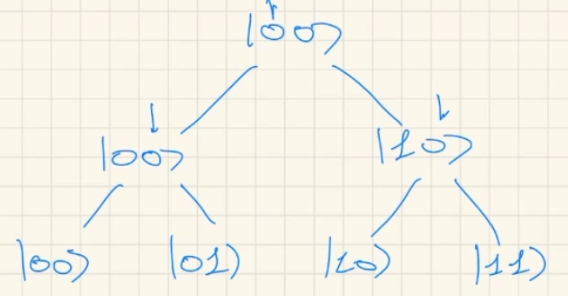
\includegraphics[scale=0.5]{41.png}
	\end{center}
In classical memory, to store 4 values we needed 8 bit. In quantum memory we need just 2 qubits.
\paragraph{FF-QRAM} Quantum memory is referred as QRAM, and FF-QRAM stands for Flip-Flop-QRAM.\\
Building QRAM follows the previous idea with another qubit that stores the value by amplitude encoding.\\
We start from a generic state 
$$\ket{Q} = \sum_{j=0}^{M-1}\psi_j\ket{j}_B\ket{0}_R$$
\begin{list}{}{}
	\item $M$ is the number of data that we want to encode
	\item $\ket{j}_B$ is the \textbf{bus register}, represents the address
	\item $\ket{0}_R$ stores the values
\end{list}
$$\ket{Q} = \frac{1}{\sqrt{M}}\sum_{j=0}^{M-1}\ket{j}_B\ket{0}_R$$
in circuit can be represented as
\begin{center}
	\begin{quantikz}
		\lstick{$\ket{0}_{B_0}$} & \gate{H} & \qw\\
		\lstick{$\ket{0}_{B_1}$} & \gate{H} & \qw\\
		\lstick{$\ket{0}_R$} & \qw & \qw
	\end{quantikz}
\end{center}
We want to load our first values on this quantum memory. Let's say we want to encode in the memory address $d_0$
$$\ket{Q} = \psi_0\ket{d_0}\ket{0}_R+\sum_{j=0,j\neq d_0}^{M-1} \psi_k\ket{j}_B\ket{0}_R$$
We amplitude encode the value $\theta_0$ in the memory address $d_0 = \ket{00}$ and $\theta_1$ in $d_1 = \ket{01}$ (the empty dot activates the control gate when the qubit is 0, the full dot activates when the qubit is 1).
\begin{center}
	\begin{quantikz}
		\lstick{$\ket{0}_{B_0}$} & \gate{H} & \octrl{1} & \qw & \octrl{1} & \qw\\
		\lstick{$\ket{0}_{B_1}$} & \gate{H} & \octrl{1} & \qw & \ctrl{1} & \qw\\
		\lstick{$\ket{0}_R$} & \qw & \gate{R_y(\theta_0)} & \qw & \gate{R_y(\theta_1)} & \qw
	\end{quantikz}
\end{center}
So we applied a controlled gate $C_{00}R_y(\theta_1)$
$$\ket{Q} = \psi_0\ket{d_0}\ket{\theta_0}_R+\sum_{j=0,j\neq d_0}^{M-1} \psi_k\ket{j}_B\ket{0}_R$$
$$\ket{\theta_0}_R = \cos\theta_0\ket{0}+\sin\theta_0\ket{1}$$
We want to encode in memory address $d_1 = \ket{01}$ the value $\theta_1$
$$\ket{Q} = \psi_0\ket{d_0}\ket{\theta_0}_R+ \psi_1\ket{d_1}\ket{\theta_1}_R+\sum_{j=0,j\neq d_0,j\neq d_1}^{M-1} \psi_k\ket{j}_B\ket{0}_R$$
The final formula is
$$\ket{Q} = \sum_{l=0}^{M-1}  \psi_{d_l}\ket{d_l}(\cos\theta_l\ket{0}_R + \sin\theta_l\ket{1}_R) + \sum_{j\not\in\{d_l\}} \psi_j\ket{j}\ket{0}_R$$
So we allocate more space than needed. If $M = 3$ we still allocate 4 memory addresses: $\theta_1, \theta_2,\theta_3$ are real data, and $\theta_4$ is a dummy value. How to manage it? We don't want the $\sum_{j=0,j\neq d_0,j\neq d_1}^{M-1} \psi_k\ket{j}_B\ket{0}_R$ part, we simply need a post selection on qubit $\ket{\:}_R$, ignoring the unused addresses.
\section{Towards a Quantum Programming Language}
\paragraph{Quantum Computation} We've seen it mostly from the point of view of gates and circuits. This covers the \textbf{data flow} aspects, but not the \textbf{control flow} aspect.\\
Selinger (2002) moves the perspective to programming languages for quantum devices, with the typical constructs: conditionals, loops\ldots in this sense we find both data flow and control flow aspects, hardware independent.\\
The slogan is "\textbf{quantum data but classical control}". In this sense, we can still exploit quantum superposition, but the control state is classical: no notion of quantum branching, no statement superposition\ldots this allows to keep things simpler. There are languages with quantum control state, but the math is heavy.\\
Also, \textbf{functional} approach: atomic and composite statements and we focus on the way in which they transform the input in the output.\\
Graphical language (flow charts) and \textbf{statically typed} (program well-formed at compile time, so no runtime checks).\\
Loops and recursion are allowed, through an intuitive denotational semantics (pictorial, visual format).\\
The \textbf{fundamental operations} are: \textbf{unitary transformations} and \textbf{measurements}.\\
Quantum algorithms interleave classical and quantum computation.
\paragraph{Hardware} Not important for now: Knull's QRAM model, classical device sends quantum circuits to a quantum device which returns some measurement. The classical controller can then decide what to do next. We assume to have some idealized hardware: no limits of memory, any unitary transformation, no noise, no error correction needed\ldots
\paragraph{Approach} States are exactly not state vectors, but they are density matrices. Several advantages: \begin{list}{}{}
	\item Pure states $\ket{\psi}$ are representable together with \textbf{mixed states} (e.g. measure, so collapse, but don't look at the measurement, getting $a_1\ket{\psi_1}+\ldots+a_n\ket{\psi_n}$ which is not a superposition)
	\item For the recursion, we need a complete partial order, state vectors do not follow it but density matrices do
	\item Abstract away from the global phase
	\item Main advantage: drastically reduce the number of square roots
\end{list} 
\pagebreak
\paragraph{Classical Flow Chart} An example\\
\tikzstyle{decision} = [diamond, draw, 
    text width=4.5em, text badly centered, node distance=3cm, inner sep=0pt]
\tikzstyle{block} = [rectangle, draw, 
    text width=5em, text centered, rounded corners, minimum height=4em]
\tikzstyle{line} = [draw, -latex']
\tikzstyle{cloud} = [draw, ellipse, node distance=3cm]
\begin{multicols}{2}
\textbf{State} of the program: $\langle$edge, $\rho\rangle$ with $\rho:$ var $\rightarrow$ Values
\begin{list}{}{}
	\item $\langle e_0,$ bc $\mapsto$ 10$\rangle$
	\item[$\mapsto$] $\langle e_2,$ bc $\mapsto$ 10$\rangle$
	\item[$\mapsto$] $\langle e_3,$ bc $\mapsto$ 00$\rangle$
	\item[$\mapsto$] $\langle e_4,$ bc $\mapsto$ 00$\rangle$
	\item[$\mapsto$] $\langle e_5,$ bc $\mapsto$ 00$\rangle$
\end{list}
\columnbreak
\begin{center}
\begin{tikzpicture}[node distance = 1cm, auto]
	\node [block] (init) {\texttt{input b,c:bit}};
	\node [decision, below of = init] (decision) {\texttt{branch b}};
	\path [line] (init) -> (decision) node [near start] {$e_0$};
	\node [block, below right of = decision, node distance=3cm] (bc) {\texttt{b := c}};
	\path [line] (decision) -> (bc) node [near start] {1}  node [near end] {$e_2$};
	\node [block, below of = bc, node distance=2cm] (c0) {\texttt{c := 0}};
	\path [line] (bc) -> (c0) node [near start] {$e_3$};
	\node [block, below left of = c0, node distance=3cm] (output) {\texttt{output b,c:bit}};
	\path [line] (c0) -> (output) node [near start] {$e_4$};
	\path [line] (decision) -> (output) node [near start] {0} node [near end] {$e_1$};
\end{tikzpicture}
\end{center}
\end{multicols}
\paragraph{Probabilistic Flow Charts} Not single value but probability distribution over values.\\
$\Gamma_0$ typing context like $b,c:$bit, syntax.\\
$A,B,C$ tuples of probabilities called annotations, semantic: $(A,B)$ corresponds to probability of first bit being 0 and first bit being 1 respectively.
$$\Gamma = A$$
\subparagraph{Syntax and Semantics}
\begin{list}{}{}
	\item \textbf{Allocate bit}
	\begin{center}
		\begin{tikzpicture}[node distance = 1cm, auto]
			\node [] (phantom1) {};
			\node [block, below of = phantom1, node distance = 1.5cm] (allocate) {\texttt{new bit b := 0}};
			\node [below of = allocate, node distance = 1.5 cm] (phantom2) {};
			\path [line] (phantom1) -> (allocate) node [near start] {$\Gamma = A$};
			\path [line] (allocate) -> (phantom2) node [near start] {\texttt{b:bit},$\Gamma = (A,0)$};
		\end{tikzpicture}
	\end{center}
	
	\item \textbf{Discard bit}
	\begin{center}
		\begin{tikzpicture}[node distance = 1cm, auto]
			\node [] (phantom1) {};
			\node [block, below of = phantom1, node distance = 1.5cm] (discard) {\texttt{discard b}};
			\node [below of = discard, node distance = 1.5 cm] (phantom2) {};
			\path [line] (phantom1) -> (discard) node [near start] {\texttt{b:bit},$\Gamma = (A,B)$};
			\path [line] (discard) -> (phantom2) node [near start] {$\Gamma = (A + B)$};
		\end{tikzpicture}
	\end{center}
	\pagebreak
	\item \textbf{Assignment}
	\begin{center}
		\begin{tikzpicture}[node distance = 1cm, auto]
			\node [] (phantom1) {};
			\node [block, below of = phantom1, node distance = 1.5cm] (assign) {\texttt{b := 1}};
			\node [below of = assign, node distance = 1.5 cm] (phantom2) {};
			\path [line] (phantom1) -> (assign) node [near start] {\texttt{b:bit},$\Gamma = (A,B)$};
			\path [line] (assign) -> (phantom2) node [near start] {$\Gamma = (0, A + B)$};
		\end{tikzpicture}
	\end{center}
	
	\item \textbf{Branching}
	\begin{center}
		\begin{tikzpicture}[node distance = 1cm, auto]
			\node [] (phantom1) {};
			\node [decision, below of = phantom1, node distance = 1.5cm] (branch) {\texttt{branch b}};
			\node [below right of = branch, node distance = 3 cm] (phantom2) {};
			\node [below left of = branch, node distance = 3 cm] (phantom3) {};
			\path [line] (phantom1) -> (branch) node [near start] {\texttt{b:bit},$\Gamma = (A,B)$};
			\path [line] (branch) -> (phantom2) node [near start] {1} node [near end] {\texttt{b:bit},$\Gamma = (0, B)$};
			\path [line] (branch) -> (phantom3) node [near start] {0} node [near end] {\texttt{b:bit},$\Gamma = (A, 0)$};
		\end{tikzpicture}
	\end{center}
	
	\item \textbf{Merge}
	\begin{center}
		\begin{tikzpicture}[node distance = 1cm, auto]
			\node [] (phantom1) {};
			\node [cloud, below right of = phantom1, node distance = 1.5cm] (merge) {};
			\node [above right of = merge, node distance = 1.5cm] (phantom2) {};
			\node [below of = merge] (phantom3) {};
			
			
			\path [line] (phantom1) -> (merge) node [near start] {$\Gamma = A$};
			\path [line] (phantom2) -> (merge) node [near start] {$\Gamma = B$};
			\path [line] (merge) -> (phantom3) node [near start] {$\Gamma = A + B$};
		\end{tikzpicture}
	\end{center}
	
	\item \textbf{Initial}
	\begin{center}
		\begin{tikzpicture}[node distance = 1cm, auto]
			\node [cloud] (init) {};
			\node [below of = init, node distance = 1.5cm] (phantom1) {};

			\path [line] (init) -> (phantom1) node [near start] {$\Gamma = 0$};
		\end{tikzpicture}
	\end{center}
	\item \textbf{Permutation}
	\begin{center}
		\begin{tikzpicture}[node distance = 1cm, auto]
			\node [] (phantom1) {$b_1,\ldots,b_n$:bit$=A_0,\ldots,A_{2^n-1}$};
			\node [block, below of = phantom1, node distance = 1.5cm] (permute) {\texttt{permute $\phi$}};
			\node [below of = permute, node distance = 1.5cm] (phantom2) {$b_{\phi(1)},\ldots,b_{\phi(n)}$:bit$=A_{2^\phi(0)},\ldots,A_{2^\phi(2^n-1)}$};

			\path [line] (phantom1) -> (permute) node [near start] {};
			\path [line] (permute) -> (phantom2) node [near start] {};
		\end{tikzpicture}
		$$\phi : \{1,\ldots,n\}\rightarrow \{1,\ldots,n\}$$
		$$2^\phi : \{0,1\}^n\rightarrow \{0,1\}^n$$
		$$2^\phi(x_1,\ldots,x_n) = (x_{\phi^{-1}(1)},\ldots,x_{\phi^{-1}(n)})$$
	\end{center}
\end{list}
\paragraph{Quantum Flow Charts} New type, \texttt{qbit}, and need to handle unitary transformations:
\begin{list}{}{}
	\item $q*=S$ apply $S$ to $q$
	\item $p,q*=S$ binary quantum transformation
	\item $q\oplus =1$ NOT
	\item $q\oplus =p$ CNOT gate, $p$ control bit
\end{list}
The output of a quantum flowchart is in general mixed state. The map associated with a QFC must send mixed states to mixed states.
\paragraph{Notation} $c\in C, \overline{c} \in C$, $C^{n\times m}$ with $n$ rows and $m$ columns.\\
$I$ identity matrix, $A= (a_{ij})_{ij}$, $A^* = (\overline{a}_{ji})_{ij}$ \textbf{conjugate transposed}\\
With $A,B,C,D\in C^{n\times m}$ we can write
$$\left(\begin{array}{c c}
A & B \\ C & D
\end{array}\right)$$
\paragraph{Trace} $tr(A) = \sum_i a_{ii}$
\subparagraph{Lemma} $tr(AB) = tr(BA)$\\
Dim: $tr(AB) = \sum_i (AB)_{ii} = \sum_i \sum_k a_{ik}b_{ki} = \sum_k\sum_i b_{ki}a_{ik} = \sum_k (BA)_{kk} = tr(BA)$
\paragraph{Norm} $|A|$ such that $|A|^2 = tr(A^*A) = \sum_{ij}\overline{a}_{ij}a_{ij}$
\paragraph{Unitary} $S^*S = I$
\subparagraph{Lemma} If $S$ is unitary, $A = SBS^*$, then $tr(A) = tr(B)\wedge |A| = |B|$
\paragraph{Hermitian Matrices} $A = A^*$\\
With $A$ Hermitian, $u^*Au\in R$. Positive Hermitian if $\forall\:u\in C^n\:\:u^*Au \geq 0$\\
$A$ Hermitian $\Leftrightarrow A = SDS^*$ for some unitary $S$ and diagonal $D$.\\
$A$ Hermitian is positive $\Leftrightarrow$ all entries of $D$ are non-negative.\\
$A$ positive $\Rightarrow |A| \leq tr(A)$\\
Remark that any positive matrix is a linear combination of positive matrices.
\paragraph{Pure Matrices} $A = VV^*$, $\ket{\psi}\bra{\psi}$ and $\cancel{\braket{\psi}{\psi}}$
\subparagraph{Theorem} Every pure matrix is positive.\\
Every positive matrix is a non-negative linear combination of pure matrices.
\paragraph{Selinger's Notation}
$$q = \alpha\mathbf{00} + \beta\mathbf{01} + \gamma\mathbf{10} + \delta\mathbf{11} = \left(\begin{array}{c}
\alpha\\\beta\\\gamma\\\delta
\end{array}\right)$$
Order is important: lexicographic order taken
\subparagraph{Unitary Transformations}
\begin{list}{}{}
	\item Create quantum superposition $H0 = \frac{1}{\sqrt{2}}\mathbf{0} + \frac{1}{\sqrt{2}}\mathbf{1}$
	\item Entanglement CNOT$(H\mathbf{0}\otimes\mathbf{0})=\frac{1}{\sqrt{2}}\mathbf{00}+\frac{1}{\sqrt{2}}\mathbf{11}$
\end{list}
\paragraph{Measurements} Capability to observe the value of a qubit and convert it into a classical bit. E.g. $q = \alpha\ket{1}+\beta\ket{1}$ has overall probability of $|\alpha|^2+|\beta|^2=1$ and we measure $q=0$ with probability $|\alpha|^2$ and $q=1=$ with probability $|\beta|^2$.\\
Given 
$$\alpha\ket{00}+\beta\ket{01}+\gamma\ket{10}+\delta\ket{11}$$
If we measure the first qubit we end up in $\alpha\ket{00}+\beta\ket{01}$ with probability $P_0=|\alpha|^2+|\beta|^2$ and in $\gamma\ket{10}+\delta\ket{11}$ with probability $P_0=|\gamma|^2+|\delta|^2$. If we measure the second qubit from $P_0$ we may end up in $\alpha\ket{00}$ with probability $P_{00}\frac{|\alpha|^2}{|\alpha|^2+|\beta|^2}$.\\
The overall probability of measuring $\alpha\ket{00}$ is $P_{0}\cdot P_{00} = |\alpha|^2$
\subparagraph{Selinger's Convention} We normalize each state in such a way that the sum of the squares of the amplitudes is equal to the overall probability that this state is reached. No necessary to renormalize each state after every measurement.\\\\
Recall that, given a state vector $u\in C^{2^n}$ of $n$ qubits that completely describes the state of the quantum system. But an external observer has only partial knowledge: may be in state $u$ or $v$ with equal probability (e.g. measure qubit but don't observe the result)
$$\frac{1}{2}\{u\}+\frac{1}{2}\{v\}$$
A \textbf{mixed state} looks like $\lambda_1\{u_1\}+\ldots+\lambda_n\{u_n\}$ with $\sum_i \lambda_i = 1$
\paragraph{Unitary Transformation for Mixed States}
$$S\left(\sum_i\lambda_i\{u_i\}\right) = \sum_i\lambda_i\{Su_i\}$$
$$q=\alpha\mathbf{0}+\beta\mathbf{1}\mapsto|\alpha|^2\{\mathbf{0}\}+|\beta|^2\{\mathbf{1}\}$$
\paragraph{Density Matrices} For a pure state we consider $u\cdot u^*$
\subparagraph{Example} $$u=\frac{1}{\sqrt{2}}\mathbf{0}-\frac{1}{\sqrt{2}}\mathbf{1}$$
$$uu^*=\left(\begin{array}{c c}
\frac{1}{\sqrt{2}}\\-\frac{1}{\sqrt{2}}
\end{array}\right)\left(\begin{array}{c c}
\frac{1}{\sqrt{2}}&-\frac{1}{\sqrt{2}}
\end{array}\right)=\left(\begin{array}{c c}
\frac{1}{\sqrt{2}}&-\frac{1}{\sqrt{2}}\\
-\frac{1}{\sqrt{2}}&\frac{1}{\sqrt{2}}
\end{array}\right)$$
Important: no essential information is lost with this transformation. If two vector differs by a global phase they have the same density matrix, but the global phase is not observable.\\
There are some advantages:
\begin{list}{}{}
	\item if $u = \gamma v$ with $|\gamma|=1$ then $uu^* = \gamma v\overline{\gamma}v^* = \gamma\overline{\gamma}vv^* = vv^*$
	\item Trace $tr(uu^*) = |u|^2$
	\item Density matrix can account for mixed states as well\\
	Given a mixed state $\sum_i \lambda_i\{u_i\}$, it's a linear combination of pure states, so the corresponding density matrix would be $\sum_i \lambda_i \{u_iu_i^*\}$
	$$\frac{1}{2}\{\mathbf{0}\}+\frac{1}{2}\{\mathbf{1}\}$$
	$$\frac{1}{2}\left(\begin{array}{c c}1&0\\0&0\end{array}\right) + \frac{1}{2}\left(\begin{array}{c c}0&0\\0&1\end{array}\right) = \left(\begin{array}{c c}\frac{1}{2}&0\\0&\frac{1}{2}\end{array}\right)$$
	\item No observable difference between two mixed states that share the same density matrix
	$$u=\frac{1}{\sqrt{2}}\mathbf{0}+\frac{1}{\sqrt{2}}\mathbf{1}\:\:\:\:\:v=\frac{1}{\sqrt{2}}\mathbf{0}-\frac{1}{\sqrt{2}}\mathbf{1}$$
	$$\frac{1}{2}\{\mathbf{u}\}+\frac{1}{2}\{\mathbf{v}\} \simeq \frac{1}{2}\{\mathbf{0}\}+\frac{1}{2}\{\mathbf{1}\}$$
\end{list}
Note: $A$ positive matrix with tr($A$) $\leq 1\Leftrightarrow A$ is a matrix in the form $\sum_i \lambda_i(u_iu_i^*)$ for unit vectors $u_i$ and non-negative coefficients $\lambda_i$ such that $\sum_i \lambda_i \leq 1$
\paragraph{Definition} A density matrix is a positive $A$ such that tr$(A)\leq 1$\\
$n$ dimensional density matrix
$$D_n\subseteq C^{n\times n}$$
\paragraph{Unitary transformations for density matrices}
$$u\mapsto Su$$
$$uu^*\mapsto Su(Su)^* = Suu^*S^*$$
Essentially $A\mapsto SAS^*$
\paragraph{Measurements on density matrices} With one vector $u=\left(\begin{array}{c}
V\\W
\end{array}\right)$ then we measure 0 collapsing to $\left(\begin{array}{c}
V\\0
\end{array}\right)$ with probability $|V|^2$ and we measure 1 collapsing to $\left(\begin{array}{c}
0\\W
\end{array}\right)$ with probability $|W|^2$.\\
With $uu^* = \left(\begin{array}{c c}
VV^*&VW^*\\WV^*&WW^*
\end{array}\right)$ we measure with probability $|V|^2=tr(VV^*)$ collapsing to $\left(\begin{array}{c c}
VV^*&0\\0&0
\end{array}\right)$ or with probability $|W|^2=tr(WW^*)$ collapsing to $\left(\begin{array}{c c}
0&0\\0&WW^*
\end{array}\right)$
\begin{center}
	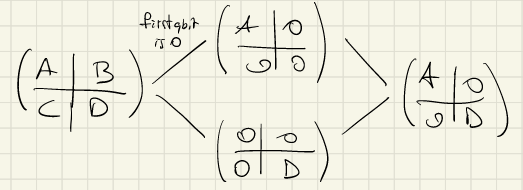
\includegraphics[scale=0.5]{43.png} %TODO scheme example
\end{center}
So measurement is also a linear transformation.
\paragraph{Complete Partial Order of Density Matrices} $D_n=\{AGC^{n\times n}\:|\: A$ positive, tr$(A)\leq 1\}$\\
We define the CPO with $A\sqsubseteq B$ if $B-A$ is positive. $B$ "improves" the precision of $A$. The bottom element is $\perp = 0$ the 0 matrix.\\
Increasing sequence $A_0 \sqsubseteq A_1\sqsubseteq\ldots\sqsubseteq A_n\sqsubseteq\ldots$, noting that the traces are also increasing and real valued, bounded by $1$ $\Rightarrow$ they have a limit $\in R$, meaning that $\{A_i\}$ will converge to some matrix.
\subsection{Quantum Flow Charts} Label $\Gamma$ typing context (syntax) and annotation $A$ density matrices (semantics). Quantum bits can be allocated (initialized to 0) and deallocated. $\overline{q}$ a finite list of quantum bits.
\paragraph{Allocate a qubit} 
	\begin{center}
		\begin{tikzpicture}[node distance = 1cm, auto]
			\node [] (phantom1) {$\Gamma = A$};
			\node [block, below of = phantom1, node distance = 1.5cm] (allocate) {\texttt{new qbit q := 0}};
			\node [below of = allocate, node distance = 1.5 cm] (phantom2) {\texttt{q:qbit},$\Gamma = \left(\begin{array}{c c} A&0\\0&0\end{array}\right)$};
			\path [line] (phantom1) -> (allocate) node [near start] {};
			\path [line] (allocate) -> (phantom2) node [near start] {};
		\end{tikzpicture}
	\end{center}
\pagebreak
\paragraph{Discard a qubit} 
	\begin{center}
		\begin{tikzpicture}[node distance = 1cm, auto]
			\node [] (phantom1) {\texttt{q:qbit},$\Gamma = \left(\begin{array}{c c} A&B\\C&D\end{array}\right)$};
			\node [block, below of = phantom1, node distance = 1.5cm] (allocate) {\texttt{discard q}};
			\node [below of = allocate, node distance = 1.5 cm] (phantom2) {$\Gamma = A + D$};
			\path [line] (phantom1) -> (allocate) node [near start] {};
			\path [line] (allocate) -> (phantom2) node [near start] {};
		\end{tikzpicture}
	\end{center}
\paragraph{Unitary transformation}
Apply $\overline{q}$\texttt{*=}$S$ ending with $\overline{q}$:qbits, $\Gamma = (S\otimes I)A(S\otimes I)^*$ (other bits stays the same with $I$)
	\begin{center}
		\begin{tikzpicture}[node distance = 1cm, auto]
			\node [] (phantom1) {\texttt{$\overline{q}$:qbits},$\Gamma = A$};
			\node [block, below of = phantom1, node distance = 1.5cm] (allocate) {\texttt{$\overline{q}$ *= S}};
			\node [below of = allocate, node distance = 1.5 cm] (phantom2) {\texttt{$\overline{q}$:qbits},$\Gamma = (S\otimes I)A(S\otimes I)^*$};
			\path [line] (phantom1) -> (allocate) node [near start] {};
			\path [line] (allocate) -> (phantom2) node [near start] {};
		\end{tikzpicture}
	\end{center}
\paragraph{Measurement}
	\begin{center}
		\begin{tikzpicture}[node distance = 1cm, auto]
			\node [] (phantom1) {\texttt{q:qbit},$\Gamma=\left(\begin{array}{cc}A&B\\C&D\end{array}\right)$};
			
			\node [below right of = branch, node distance = 3 cm] (phantom2) {\texttt{q:qbit},$\Gamma=\left(\begin{array}{cc}0&0\\0&D\end{array}\right)$};
			\node [below left of = branch, node distance = 3 cm] (phantom3) {\texttt{q:qbit},$\Gamma=\left(\begin{array}{cc}A&0\\0&0\end{array}\right)$};
			\path [line] (phantom1) -> (branch) node [near start] {};
			\path [line] (branch) -> (phantom2);
			\path [line] (branch) -> (phantom3);
		\end{tikzpicture}
	\end{center}
\paragraph{Merge} 
	\begin{center}
		\begin{tikzpicture}[node distance = 1cm, auto]
			\node [] (phantom1) {$\Gamma = A$};
			\node [cloud, below right of = phantom1, node distance = 1.5cm] (merge) {};
			\node [above right of = merge, node distance = 1.5cm] (phantom2) {$\Gamma = B$};
			\node [below of = merge] (phantom3) {$\Gamma = A+B$};
			\path [line] (phantom1) -> (merge) node [near start] {};
			\path [line] (phantom2) -> (merge) node [near start] {};
			\path [line] (merge) -> (phantom3) node [near start] {};
		\end{tikzpicture}
	\end{center}
\paragraph{Initialization}
	\begin{center}
		\begin{tikzpicture}[node distance = 1cm, auto]
			\node [cloud] (init) {};
			\node [below of = init, node distance = 1.5cm] (phantom1) {};

			\path [line] (init) -> (phantom1) node [near start] {$\Gamma = 0$};
		\end{tikzpicture}
	\end{center}
\pagebreak
\paragraph{Permutation}
	\begin{center}
		\begin{tikzpicture}[node distance = 1cm, auto]
			\node [] (phantom1) {$q_1,\ldots,q_n$:qbits$=(a_{ij})_{ij}$};
			\node [block, below of = phantom1, node distance = 1.5cm] (permute) {\texttt{permute $\phi$}};
			\node [below of = permute, node distance = 1.5cm] (phantom2) {$q_{\phi(1)},\ldots,q_{\phi(n)}$:qbits$=(a_{2^\phi(i)2^\phi(j)})_{ij}$};

			\path [line] (phantom1) -> (permute) node [near start] {};
			\path [line] (permute) -> (phantom2) node [near start] {};
		\end{tikzpicture}
	\end{center}
\paragraph{Example}
\begin{center}
		\begin{tikzpicture}[node distance = 2cm, auto]
			\node [] (ph1) {\texttt{q:qbit},$\Gamma=\left(\begin{array}{c c}A&B\\C&D\end{array}\right)$};
			\node [decision, below of = ph1] (branch) {\texttt{measure q}};
			\node [below left of = branch, node distance = 3 cm] (m0) {\texttt{q:qbit},$\Gamma=\left(\begin{array}{c c}A&0\\0&0\end{array}\right)$};
			\node [below right of = branch, node distance = 3 cm] (m1) {\texttt{q:qbit},$\Gamma=\left(\begin{array}{c c}0&0\\0&D\end{array}\right)$};
			\node [block, below of = m1] (not) {\texttt{q $\oplus$= 1}\\(not gate)};
			\node [below of = not] (notres) {\texttt{q:qbit},$\Gamma=\left(\begin{array}{c c}D&0\\0&0\end{array}\right)$};
			\node [cloud, below left of = notres] (merge) {};
			\node [below of = merge] (end) {\texttt{q:qbit},$\Gamma=\left(\begin{array}{c c}A+D&0\\0&0\end{array}\right)$};
			
			\path [line] (ph1) -> (branch);
			\path [line] (branch) -- (m0);
			\path [line] (m0) -> (merge);
			\path [line] (branch) -- (m1);
			\path [line] (m1) -- (not);
			\path [line] (not) -- (notres);
			\path [line] (notres) -- (merge);
			\path [line] (merge) -- (end);
		\end{tikzpicture}
	
\end{center}
\pagebreak
\paragraph{Combining classical data with quantum data} Classical data corresponds to control paths, quantum data to quantum paths.\\
In the combined language, we have two data types: bit and qubit. The typing context are those defined before. An edge with $n$ bits and $m$ qubits can be replaced by $2^n$ edges (all combinations of the bits) labeled with $m$ qubits only.\\
A typing context $\Gamma$ is a $2^n$ tuple $(A_0,\ldots, A_{2^n-1})$ of density matrices, each of dimension $2^n\times 2^n$.\\\\
$$tr(A_0,\ldots,A_{2^n-1}) = \sum_{i=0}^{2^n-1} tr(A_i)$$
$$(A_0,\ldots,A_{2^n-1})^* = (A_0^*,\ldots,A_{2^n-1}^*)$$
$$S(A_0,\ldots,A_{2^n-1}) = (SA_0,\ldots,SA_{2^n-1})$$
$$|(A_0,\ldots,A_{2^n-1})|^2 = \sum_{i=0}^{2^n-1} |A_i|^2$$
Flow charts are acyclic graphs whose edges are typed with typing contexts, and whose nodes can be any of the previously seen components.
\subparagraph{Property} The annotation of a flowchart is uniquely determined by the annotation of its input edges. Calculated in a top-down fashion apply the rules we've seen.\\
To each flowchart is associated a linear transformation from its input to its output edges, because we've seen only linear transformations and composing them linearly preserve the linearity. This linear function preserver both positivity and traces (the sum of input traces equals to the sum of output traces). Without loops only!
\paragraph{Examples}
\begin{center}
		\begin{tikzpicture}[node distance = 2cm, auto]
			\node [] (ph1) {\texttt{q:qbit},$\Gamma=\left(\begin{array}{c c}A&B\\C&D\end{array}\right)$};
			\node [decision, below of = ph1] (branch) {\texttt{measure q}};
			\node [below left of = branch, node distance = 3 cm] (m0) {\texttt{q:qbit},$\Gamma=\left(\begin{array}{c c}A&0\\0&0\end{array}\right)$};
			\node [below right of = branch, node distance = 3 cm] (m1) {\texttt{q:qbit},$\Gamma=\left(\begin{array}{c c}0&0\\0&D\end{array}\right)$};
			\node [cloud, below left of = m1] (merge) {};
			\node [below of = merge] (state) {\texttt{q:qbit},$\Gamma=\left(\begin{array}{c c}A&0\\0&D\end{array}\right)$};
			\node [block, below of = state] (discard) {\texttt{discard q}};
			\node [below of = discard] (end) {$\Gamma=A+D$};
			
			\path [line] (ph1) -> (branch);
			\path [line] (branch) -> (m0);
			\path [line] (branch) -> (m1);
			\path [line] (m0) -> (merge);
			\path [line] (m1) -> (merge);
			\path [line] (merge) -> (state);
			\path [line] (state) -> (discard);
			\path [line] (discard) -> (end);
			
		\end{tikzpicture}
	
\end{center}
\pagebreak
Another example: $\forall\:x$ flow char

\begin{center}
		\begin{tikzpicture}[node distance = 2cm, auto]
			\node [] (ph1) {\texttt{q:qbit},$\Gamma_1$};
			\node [block, below of = ph1] (discard1) {\texttt{discard q}};
			\path [line] (ph1) -> (discard1);
			\node [below of = discard1] (state1) {$\Gamma_1$};
			\path [line] (discard1) -> (state1);
			\node [right of = ph1] (phdots) {\ldots};
			\node [right of = phdots] (phn) {\texttt{q:qbit},$\Gamma_n$};
			\node [block, below of = phn] (discardn) {\texttt{discard q}};
			\path [line] (phn) -> (discardn);
			\node [below of = discardn] (staten) {$\Gamma_n$};
			\path [line] (discardn) -> (staten);
			
			\node [block, below of = phdots, node distance = 5.5 cm] (X) {$X$};
			\path [line] (state1) -> (X);
			\path [line] (staten) -> (X);
			
			\node [below left of = X] (end1) {$\Delta_1$};
			\path [line] (X) -> (end1);
			\node [below of = X] (enddots) {\ldots};
			\node [below right of = X] (endn) {$\Delta_n$};
			\path [line] (X) -> (endn);
		\end{tikzpicture}
\end{center}
\textbf{Loops} can be realized with this:
\begin{center}
		\begin{tikzpicture}[node distance = 2cm, auto]
			\node [cloud] (merge) {};
			\node [above left of = merge, node distance = 3 cm] (ph1) {$A$};
			\path [line] (ph1) -> (merge);
			\node [above right of = merge] (ph21) {};
			\node [right of = ph21] (ph22) {};
			\path [line] (ph21) -> (merge);
			\path [line] (ph22) -> (ph21);
			\node [decision, below of = merge, node distance = 1.5 cm] (branch) {\texttt{measure}};
			\path [line] (merge) -> (branch);
			\node [below left of = branch] (false) {};
			\path [line] (branch) -> (false);
			\node [below of = false, node distance = 3 cm] (end) {$G(A)$};
			\path [line] (false) -> (end);
			\node [block, below right of = branch] (true) {$X$};
			\path [line] (branch) -> (true);
			\node [below of = true] (ph24) {};
			\path [line] (true) -> (ph24);
			\node [right of = ph24] (ph23) {};
			\path [line] (ph24) -> (ph23);
			\path [line] (ph23) -> (ph22);
		\end{tikzpicture}
\end{center}
\subsection{Quantum Imperative Programming Language}
\paragraph{Classical Imperative Programming Language} Many familiar commands: \texttt{S ::=}
\begin{list}{}{}
	\item \texttt{skip} does nothing
	\item \texttt{u := t} assignment, $u$ variable and $t$ expression
	\item \texttt{s1;s2} sequential composition
	\item \texttt{if b then s1 else s2 fi} conditional, with $b$ boolean expression
	\item \texttt{while b do s od} loop, again $b$ boolean expression
\end{list}
In order to move to the quantum world, we need to \textbf{generalize the conditional statement}.
\subparagraph{Generalized Conditional Statement} \begin{list}{}{}
	\item \texttt{if G1 $\rightarrow$ S1}
	\item \texttt{$\square$ G2 $\rightarrow$ S2}
	\item \ldots
	\item \texttt{$\square$ Gn $\rightarrow$ Sn}
	\item \texttt{fi}
\end{list}
With $G_i$ boolean expression and \textbf{only the first $S_i$ which $G_i$ holds true is executed}.\\
\texttt{if ($\underset{i}{\square}$ Gi $\rightarrow$ Si) fi}
\paragraph{\texttt{qVar}} Set of quantum variables, ranged over by \texttt{q, q', q0,\ldots}, each \texttt{q} $\in$ Var has values in $H_2$.\\
$\overline{q}$ denotes a quantum register, a finite sequence of \textbf{distinct} variables in \texttt{qVar}.
\begin{list}{}{}
	\item $\overline{q}\in H_{\overline{q}} = \bigotimes_{i=1}^n H_{q_i}$
	\item $H_{all} = \bigotimes_{q\in\hbox{qVar}} H_q$ Hilbert space of all quantum variables
	\item $\ket{\psi}_{q_i}$ denotes that $\ket{\psi}$ is the state of the variable $q_i$\\
	We extend this notation to $\ket{\psi}_{q_i}\bra{\phi}$ outer produt of state $\ket{\psi}$ and $\ket{\phi}$ of $q_i$\\
	In general the state of a quantum register in $H_{\overline{q}}$ is $\ket{\psi_1}_{q_1}\ldots\ket{\psi_n}_{q_n}$ if each $q_i$ is in its state $\ket{\psi_i}$ for every $1\leq i\leq n$
	\item $\overline{q} = q_1\ldots q_n$, $A$ operator in $H_{\overline{q}}$ has a cylindrical extension $A\otimes I$ that operates in $H_{all}$, where $I$ is the identity operator $\bigotimes_{q\in\hbox{qVar}\setminus \overline{q}} H_q$\\
	For brevity we shall write $A$ in place of $A\otimes I$
\end{list}
\subsubsection{Quantum Programs}
\texttt{S::=}
\begin{list}{}{}
	\item \texttt{skip} does nothing
	\item \texttt{q:=$\ket{0}$} sets $q$ to the initial state $\ket{0}$
	\item \texttt{$\overline{q}$:=U[$\overline{q}$]} applies the unitary transformation $U$ to the register $\overline{q}$
	\item \texttt{S1;S2} sequential composition
	\item \texttt{if ($\underset{m}{\square}$ M[$\overline{q}$] = $m\rightarrow$ S$m$) fi} quantum case statement %TODO explanation
	\item \texttt{while M[$\overline{q}$] = 1 do S od} quantum loop\\
	Yes/true is 1 and no/false is 0
\end{list}
Note: for any state $\ket{\psi}$ we can find a unitary transformation $U$ such that with \texttt{q:=$\ket{0}$;q:=U[q]} we get \texttt{q=$\ket{\psi}$}, so being able to initialize exclusively to $\ket{0}$ is not a limitation.\\
Also note $M = \{M_m\} = \{M_{m_1},\ldots,M_{m_n}\}$ is a family of measurements.
\paragraph{Difference with the classical case for conditionals} The state of the program is changed after performing the measure.\\
"\textbf{Quantum data, classical flow}", referring to conditional and loops: in order to make a decision we must make a measure.
\paragraph{•} \texttt{qvar : S $\rightarrow$ P(qVar)} variables appearing in a statement. For example:
\begin{list}{}{}
	\item qvar(skip) = emptyset
	\item qvar(q:=|0>) = \{q\}
	\item qvar($\overline{q}$:=U[$\overline{q}$]) = $\overline{q}$
	\item qvar(\texttt{S1;S2}) = qvar(\texttt{S1}) $\cup$ qvar(\texttt{S2})
	\item qvar(\texttt{if ($\underset{m}{\square}$ M[$\overline{q}$] = $m\rightarrow$ S$m$) fi}) = $\overline{q}\cup\bigcup_m$ qvar(\texttt{S$m$})
	\item qvar(\texttt{while M[$\overline{q}$] = 1 do S od}) = $\overline{q}\cup$ qvar(\texttt{S})
\end{list}
Given a statement \texttt{S}, $H_{all}$ can be understood as $H_{qvar(\texttt{S})}$
\paragraph{Quantum Configuration} $\langle \texttt{S},\rho\rangle$ where
\begin{list}{}{}
	\item \texttt{S} is a quantum statement or, taking into account the termination of the computation, the special statement for the empty program ($\epsilon$)\\
	$\langle \texttt{S},\rho\rangle$ = nothing to be done, terminated in state $\rho$
	\item $\rho\in D(H_{all})$ is a partial density operators denoting the global state of quantum variables.\\
	$tr(\rho)=1\Rightarrow$ density operator, $tr(\rho)\leq 1\Rightarrow$ partial density operator.\\
	$D(H)$ is the sate of all partial density operators of Hilbert space $H$
\end{list}
\paragraph{Small Step Semantics} Transition system $\langle \texttt{S}, \rho\rangle\rightarrow\langle\texttt{S}',\rho'\rangle$\\
Transition between configurations to be read as "after executing one step of \texttt{S} in $\rho$, we reach the state $\rho'$ where $\texttt{S}'$ is yet to be executed. If $\texttt{S}'=\epsilon$, then the program terminates in state $\rho'$.
\subparagraph{Inference Rules} Induction on the structure of the statements.
$$\frac{\hbox{premises}}{\hbox{conclusion}}$$
To be read as "if the premises hold, then the conclusion is true".\\
Some \textbf{axioms}, rules without premises:
\begin{list}{}{}
	\item[(\texttt{SK})] $\frac{\hbox{}}{\langle\texttt{skip},\rho\rangle\rightarrow\langle\epsilon,\rho\rangle}$
	\item[(\texttt{IN})] $\frac{\hbox{}}{\langle\texttt{q:=}\ket{0},\rho\rangle\rightarrow\langle\epsilon,\rho_0^q\rangle}$ with $rho_0^q = \ket{0}_q\bra{0}\rho\ket{0}_q\bra{0} + \ket{0}_q\bra{1}\rho\ket{1}_q\bra{0}$ (transform all zero of $q$ into zero and all ones of $q$ into ones) %TODO format
	\item[(\texttt{UT})] $\frac{}{\langle \overline{q}\texttt{:=U[}\overline{q}\texttt{]},\rho\rangle\rightarrow\langle\epsilon U\rho U^*\rangle}$
	\item[(\texttt{SC}] $\frac{\langle \texttt{S1},\rho\rangle\rightarrow\langle \texttt{S1}',\rho'\rangle}{\langle\texttt{S1;S2},\rho\rangle\rightarrow\langle\texttt{S1}'\texttt{;S2},\rho'\rangle}$\\
	Special case for $\texttt{S1}' = \epsilon$ %TODO
	\item[(\texttt{IF})]
	\item[(\texttt{LO})]
	\item[(\texttt{LI})]
	\item[(\texttt{IF$'$})]
\end{list}
Non-deterministic rotation system.
\paragraph{Denotational Semantics} Assign the transformation function from input to output for every statement. We exploit %TODO
We look at all the possible executions %TODO
We write $$\langle S,\rho\rangle\rightarrow^n\langle S', \rho'\rangle \Leftrightarrow \langle S,\rho\rangle\rightarrow \langle S_1,\rho_1\rangle\rightarrow\ldots\rightarrow\langle S_{n-1},\rho_{n-q}\rangle\rightarrow\langle S',\rho'\rangle$$
$$\langle S,\rho\rangle\rightarrow^*\langle S',\rho'\rangle\Leftrightarrow\exists\:n\in\mathbb{N}\langle S,\rho\rangle\rightarrow^n\langle S',\rho'\rangle$$
$[S] : D(H_{all})\rightarrow D(H_{all})$ defined by the following
$$[S]\rho =\sum\{\rho'\:|\:\langle S,\rho\rangle\rightarrow^*\langle\epsilon,\rho'\rangle\}$$
Important to account for all paths. \textbf{Lemma}: it's a linear function. Proof by structural induction, all the transformations applied at each steps are linear.
\paragraph{Theorem} $[\texttt{while M[q] = 1 do S od}]\rho = M_0\rho M_0^* + [\texttt{while M[q] = 1 do S od}]([S]M_1\rho M_1^*)$\\
So it's equal to stopping now or appling to the resulting state.
\paragraph{Prop} Remembering that the trace is the overall probability, in general with non-terminating paths $tr([S]\rho) \leq tr(\rho)$\\
Intuitively, $tr([S]\rho)$ is the probability of termination from $\rho$, meaning that the probability of divergence is\\$tr(\rho)-tr([S]\rho)$.
\paragraph{Hoare Triples in Classical Programming Recap} $$\{P\}S\{Q\}$$
For any input that satisfies the predicate $P$, the execution of $S$ will produce an output that satisfies $Q$
\pagebreak
\paragraph{Quantum Predicate} In classical logic, a predicate expresses some properties of individuals or systems. In the quantum world, a quantum predicate must be something that we can physically observe.\\
In general, we take an Hermitian operator $M$ in its Hilbert space $H$ and we know that $$M\ket{\phi}=\lambda\ket{\psi}$$ with $\lambda\in\mathbb{R}$ eigenvalues and $\psi$ eigenvector. The eigenspace is
$$X_\lambda=\{\ket{\psi}\in H\:|\:M\ket{\phi} = \lambda\ket{\psi}\}$$ and $\lambda$ can be understood as the truth value of the propositions in $X_\lambda$. We can restrict the eigenspace in the range $[0,1]$ by requiring $0\leq \lambda\leq 1$
\subparagraph{Definition} A \textbf{quantum predicate} in a Hilbert space $H$ is an Hermitian operator $M\in H$ such that all its eigenvalues lay within the interval $[0,1]$.\\
$P(H)$ is the set of quantum predicates over $H$.\\
$tr(M\rho)$ is the expectation of the value of the measurement outcome of observable $M$ in a mixed state $\rho$. The average truth value of the predicate $M$ in $\rho$. Of course it's $0\leq tr(M\rho)\leq 1$.
\subparagraph{Lemma} $M\sqsubseteq N \Leftrightarrow \forall\:\rho\:\:tr(M\rho)\leq tr(N\rho)$
\paragraph{Weakest Precondition} The weakest property that the input must satisfy in order to achieve a given property of the output.\\
In the quantum setting: given two quantum predicates $M,N\in P(H)$ and $\epsilon$ quantum operator (typically the semantics of some statements $\epsilon = [S]$), we write $\{M\}\epsilon\{N\}$ if $\forall\:\rho\in D(H)\:\: tr(M\rho)\leq tr(N\epsilon\rho)$\\
If the state $\rho$ satisfies $M$, then $\epsilon\rho$ satisfies $N$\\
$wp(\epsilon)(N)$ is the weakest precondition of $N$ with respect to the transformation $\epsilon$ if:\begin{list}{}{}
	\item is itself a precond $\{wp(\epsilon)(N)\}\epsilon\{N\}$
	\item $\forall\:\{M\}\epsilon\{N\}\Rightarrow M\sqsubseteq wp(\epsilon)(N)$ so any other precondition is weaker
\end{list}
\paragraph{Correctness}
\begin{list}{}{}
	\item \textbf{Total Correctness} $vDash_{tot}\{P\}S\{Q\}\equiv\{P\}[S]\{Q\}$ if $\forall\:\rho\in D(H_{all}) tr(P\rho)\leq tr(Q[S]\rho)$ 
	\item \textbf{Partial} $vDash_{par}\{P\}S\{Q\}$ if $tr(P\rho)\leq tr(Q[S]\rho)+(\underset{\hbox{divergence probability}}{tr(\rho)-tr([S]\rho)})$ accounts for divergence\\
	Intuitively, if input $\rho$ satisfies the precondition $P$ then either $S$ terminates on $\rho$ and $[S]\rho$ satisfies $Q$ or $S$ diverges on $\rho$
\end{list}
These relations are also linear: for both total or partial, $vDash\{P_i\}S\{Q_i\}$ for $i=1,2$ then $\{\lambda_1P_1+\lambda_2P_2\}S\{\lambda_1Q_1+\lambda_2Q_2\}$ for any $\lambda_1,\lambda_2$ %TODO
\paragraph{Proof System for Partial Correctness} There are a set of rules to derive partial correctness (for total too but it's far more complicated). Allows to derive all and only %TODO
\begin{list}{}{}
	\item[(Ax-SK)]
	\item[(Ax-UT)]
	\item[(R-SC)]
	\item[(R-IF)]
	\item[(R-LP)]
	\item[(R-OP)]
\end{list}
\end{document}  
